

% uWaterloo Thesis Template for LaTeX 
% Last Updated May 24, 2011 by Stephen Carr, IST Client Services
% FOR ASSISTANCE, please send mail to rt-IST-CSmathsci@ist.uwaterloo.ca

% Effective October 2006, the University of Waterloo 
% requires electronic thesis submission. See the uWaterloo thesis regulations at
% http://www.grad.uwaterloo.ca/Thesis_Regs/thesistofc.asp.

% DON'T FORGET TO ADD YOUR OWN NAME AND TITLE in the "hyperref" package
% configuration below. THIS INFORMATION GETS EMBEDDED IN THE PDF FINAL PDF DOCUMENT.
% You can view the information if you view Properties of the PDF document.

% Many faculties/departments also require one or more printed
% copies. This template attempts to satisfy both types of output. 
% It is based on the standard "book" document class which provides all necessary 
% sectioning structures and allows multi-part theses.

% DISCLAIMER
% To the best of our knowledge, this template satisfies the current uWaterloo requirements.
% However, it is your responsibility to assure that you have met all 
% requirements of the University and your particular department.
% Many thanks to the feedback from many graduates that assisted the development of this template.

% -----------------------------------------------------------------------

% By default, output is produced that is geared toward generating a PDF 
% version optimized for viewing on an electronic display, including 
% hyperlinks within the PDF.
 
% E.g. to process a thesis called "mythesis.tex" based on this template, run:

% pdflatex mythesis	-- first pass of the pdflatex processor
% bibtex mythesis	-- generates bibliography from .bib data file(s) 
% pdflatex mythesis	-- fixes cross-references, bibliographic references, etc
% pdflatex mythesis	-- fixes cross-references, bibliographic redeferences, etc

% If you use the recommended LaTeX editor, Texmaker, you would open the mythesis.tex
% file, then click the pdflatex button. Then run BibTeX (under the Tools menu).
% Then click the pdflatex button two more times. If you have an index as well,
% you'll need to run MakeIndex from the Tools menu as well, before running pdflatex
% the last two times.

% N.B. The "pdftex" program allows graphics in the following formats to be
% included with the "\includegraphics" command: PNG, PDF, JPEG, TIFF
% Tip 1: Generate your figures and photos in the size you want them to appear
% in your thesis, rather than scaling them with \includegraphics options.
% Tip 2: Any drawings you do should be in scalable vector graphic formats:
% SVG, PNG, WMF, EPS and then converted to PNG or PDF, so they are scalable in
% the final PDF as well.
% Tip 3: Photographs should be cropped and compressed so as not to be too large.

% To create a PDF output that is optimized for double-sided printing: 
%
% 1) comment-out the \documentclass statement in the preamble below, and
% un-comment the second \documentclass line.
%
% 2) change the value assigned below to the boolean variable
% "PrintVersion" from "false" to "true".

% --------------------- Start of Document Preamble -----------------------

% Specify the document class, default style attributes, and page dimensions
% For hyperlinked PDF, suitable for viewing on a computer, use this:
\documentclass[letterpaper,12pt,titlepage, english, openright]{book}
\setcounter{secnumdepth}{3}  %% Avec un numero.
\setcounter{tocdepth}{2}   
 \hyphenation{op-tical net-works semi-conduc-tor}
 \usepackage[linesnumbered,ruled,vlined]{algorithm2e}
 \usepackage[pdftex]{graphicx} 
 %\usepackage{stfloats}
 \usepackage{cite}
 \usepackage[cmex10]{amsmath}
 \usepackage{algorithmic}
 \usepackage{multirow}
 %\fnbelowfloat
 \usepackage[tight,footnotesize]{subfigure}
 \usepackage{listings}
 \usepackage{color}
 \usepackage{url}
 \definecolor{dkgreen}{rgb}{0,0.6,0}
 \definecolor{gray}{rgb}{0.5,0.5,0.5}
 \definecolor{mauve}{rgb}{0.58,0,0.82}
 \usepackage{multirow}
 \usepackage{booktabs}
 \usepackage{amsthm}
 \usepackage{hhline}
 \newtheorem*{remark}{Remark}
 \usepackage{calc}
 \usepackage{amssymb}
 \usepackage{epstopdf}
 \lstset{frame=tb,
 	language=Java,
 	aboveskip=3mm,
 	belowskip=3mm,
 	showstringspaces=false,
 	columns=flexible,
 	basicstyle={\small\ttfamily},
 	numbers=none,
 	numberstyle=\tiny\color{gray},
 	keywordstyle=\color{blue},
 	commentstyle=\color{dkgreen},
 	stringstyle=\color{mauve},
 	tabsize=3
 }
 %\usepackage{titlesec}
\usepackage{float}
 \usepackage{placeins}
 \setcounter{topnumber}{10}
 \setcounter{bottomnumber}{10}
 \setcounter{totalnumber}{10}
 \renewcommand{\floatpagefraction}{.9}
 \renewcommand{\textfraction}{.2}
 \DeclareGraphicsExtensions{.pdf,.png,.jpg,.mps} 
 \usepackage{lipsum}
 
 \usepackage{etoolbox}
 \usepackage{fancyhdr}
 \usepackage{kantlipsum}
% For PDF, suitable for double-sided printing, change the PrintVersion variable below
% to "true" and use this \documentclass line instead of the one above:
%\documentclass[letterpaper,12pt,titlepage,openright,twoside,final]{book}

% Some LaTeX commands I define for my own nomenclature.
% If you have to, it's better to change nomenclature once here than in a 
% million places throughout your thesis!
\newcommand{\package}[1]{\textbf{#1}} % package names in bold text
\newcommand{\cmmd}[1]{\textbackslash\texttt{#1}} % command name in tt font 
\newcommand{\href}[1]{#1} 
\newcommand{\ie}{\emph{i.e.}\xspace}
\newcommand{\eg}{\emph{e.g.}}
\newcommand{\cf}{\emph{cf.}}
\newcommand{\etal}{\emph{et al.}\xspace}

% does nothing, but defines the command so the
    % print-optimized version will ignore \href tags (redefined by hyperref pkg).
%\newcommand{\texorpdfstring}[2]{#1} % does nothing, but defines the command
% Anything defined here may be redefined by packages added below...

% This package allows if-then-else control structures.
\usepackage{ifthen}
\newboolean{PrintVersion}
\setboolean{PrintVersion}{false} 
% CHANGE THIS VALUE TO "true" as necessary, to improve printed results for hard copies
% by overriding some options of the hyperref package below.

%\usepackage{nomencl} % For a nomenclature (optional; available from ctan.org)
\usepackage{amsmath,amssymb,amstext} % Lots of math symbols and environments
\usepackage[pdftex]{graphicx} % For including graphics N.B. pdftex graphics driver 

% Hyperlinks make it very easy to navigate an electronic document.
% In addition, this is where you should specify the thesis title
% and author as they appear in the properties of the PDF document.
% Use the "hyperref" package 
% N.B. HYPERREF MUST BE THE LAST PACKAGE LOADED; ADD ADDITIONAL PKGS ABOVE
\usepackage[pdftex,letterpaper=true,pagebackref=false]{hyperref} % with basic options
		% N.B. pagebackref=true provides links back from the References to the body text. This can cause trouble for printing.
\hypersetup{
    plainpages=false,       % needed if Roman numbers in frontpages
    pdfpagelabels=true,     % adds page number as label in Acrobat's page count
    bookmarks=true,         % show bookmarks bar?
    unicode=false,          % non-Latin characters in Acrobat’s bookmarks
    pdftoolbar=true,        % show Acrobat’s toolbar?
    pdfmenubar=true,        % show Acrobat’s menu?
    pdffitwindow=false,     % window fit to page when opened
    pdfstartview={FitH},    % fits the width of the page to the window
    pdftitle={uWaterloo\ LaTeX\ Thesis\ Template},    % title: CHANGE THIS TEXT!
%    pdfauthor={Author},    % author: CHANGE THIS TEXT! and uncomment this line
%    pdfsubject={Subject},  % subject: CHANGE THIS TEXT! and uncomment this line
%    pdfkeywords={keyword1} {key2} {key3}, % list of keywords, and uncomment this line if desired
    pdfnewwindow=true,      % links in new window
    colorlinks=true,        % false: boxed links; true: colored links
    linkcolor=blue,         % color of internal links
    citecolor=green,        % color of links to bibliography
    filecolor=magenta,      % color of file links
    urlcolor=cyan           % color of external links
}
\ifthenelse{\boolean{PrintVersion}}{   % for improved print quality, change some hyperref options
\hypersetup{	% override some previously defined hyperref options
%    colorlinks,%
    citecolor=black,%
    filecolor=black,%
    linkcolor=black,%
    urlcolor=black}
}{} % end of ifthenelse (no else)

% Setting up the page margins...
% uWaterloo thesis requirements specify a minimum of 1 inch (72pt) margin at the
% top, bottom, and outside page edges and a 1.125 in. (81pt) gutter
% margin (on binding side). While this is not an issue for electronic
% viewing, a PDF may be printed, and so we have the same page layout for
% both printed and electronic versions, we leave the gutter margin in.
% Set margins to minimum permitted by uWaterloo thesis regulations:
\setlength{\marginparwidth}{0pt} % width of margin notes
% N.B. If margin notes are used, you must adjust \textwidth, \marginparwidth
% and \marginparsep so that the space left between the margin notes and page
% edge is less than 15 mm (0.6 in.)
\setlength{\marginparsep}{0pt} % width of space between body text and margin notes
\setlength{\evensidemargin}{0.125in} % Adds 1/8 in. to binding side of all 
% even-numbered pages when the "twoside" printing option is selected
\setlength{\oddsidemargin}{0.125in} % Adds 1/8 in. to the left of all pages
% when "oneside" printing is selected, and to the left of all odd-numbered
% pages when "twoside" printing is selected
\setlength{\textwidth}{6.375in} % assuming US letter paper (8.5 in. x 11 in.) and 
% side margins as above
\raggedbottom

% The following statement specifies the amount of space between
% paragraphs. Other reasonable specifications are \bigskipamount and \smallskipamount.
\setlength{\parskip}{\medskipamount}

% The following statement controls the line spacing.  The default
% spacing corresponds to good typographic conventions and only slight
% changes (e.g., perhaps "1.2"), if any, should be made.
\renewcommand{\baselinestretch}{1} % this is the default line space setting

% By default, each chapter will start on a recto (right-hand side)
% page.  We also force each section of the front pages to start on 
% a recto page by inserting \cleardoublepage commands.
% In many cases, this will require that the verso page be
% blank and, while it should be counted, a page number should not be
% printed.  The following statements ensure a page number is not
% printed on an otherwise blank verso page.
\let\origdoublepage\cleardoublepage
\newcommand{\clearemptydoublepage}{%
  \clearpage{\pagestyle{empty}\origdoublepage}}
\let\cleardoublepage\clearemptydoublepage

%======================================================================
%   L O G I C A L    D O C U M E N T -- the content of your thesis
%======================================================================
%=========================GPCEEEEEEEEEEEE
\newcommand{\cL}{{\cal L}}


\usepackage{standalone}

\usepackage[table]{xcolor}
\usepackage{hhline}

\hyphenation{op-tical net-works semi-conduc-tor}
\usepackage[linesnumbered,ruled,vlined]{algorithm2e}
\usepackage[pdftex]{graphicx}
\usepackage{siunitx}
\sisetup{binary-units = true}

%\usepackage{stfloats}
%\usepackage{cite}
\usepackage{amsthm}
 
\usepackage{algorithmic}
\usepackage{multirow}
%\fnbelowfloat
\usepackage[tight,footnotesize]{subfigure}
\usepackage{listings}
\usepackage{color}
\usepackage{url}
\definecolor{dkgreen}{rgb}{0,0.6,0}
\definecolor{gray}{rgb}{0.5,0.5,0.5}
\definecolor{mauve}{rgb}{0.58,0,0.82}

\lstset{frame=tb,
	language=Java,
	aboveskip=3mm,
	belowskip=3mm,
	showstringspaces=false,
	columns=flexible,
	basicstyle={\small\ttfamily},
	numbers=none,
	numberstyle=\tiny\color{gray},
	keywordstyle=\color{blue},
	commentstyle=\color{dkgreen},
	stringstyle=\color{mauve},
	tabsize=3
}


\setcounter{topnumber}{10}
\setcounter{bottomnumber}{10}
\setcounter{totalnumber}{10}
\renewcommand{\floatpagefraction}{.9}
\renewcommand{\textfraction}{.2}
\DeclareGraphicsExtensions{.pdf,.png,.jpg,.mps} 

\usepackage{amsthm}
\newtheorem*{mydef}{Definition}

\renewcommand{\floatpagefraction}{.9}
\renewcommand{\textfraction}{.1}
\renewcommand{\topfraction}{.8}
\renewcommand{\bottomfraction}{.8}
\newcommand*{\tabref}[1]{\tablename~\ref{#1}}
\newcommand*{\figref}[1]{\figurename~\ref{#1}}




%% choix des profondeurs de section pour la table des matières
%% 2= subsection, 3=subsubsection
\setcounter{secnumdepth}{3}  %% Avec un numero.
\setcounter{tocdepth}{2}     %% Visibles dans la table des matieres
\makeindex %% crée l'index
\usepackage{pdfpages}



\begin{document}

\addtocounter{page}{-1}%ça c'est pour revenir à 0
%\fontfamilly{phv}

%%  1ere de Couverture:
%\documentclass[11pt, english, openright]{book}
\usepackage{etex}
%% En 12pt c'est possible aussi
%% packages utilises
%%---------------------
\usepackage[utf8]{inputenc}
\usepackage[T1]{fontenc}
\usepackage{amsmath}
\usepackage{listings}
%\usepackage{math}
\usepackage{amssymb}
\usepackage{these}
\usepackage{setspace}
\usepackage{emptypage}
 \usepackage{array}
\usepackage[inline]{enumitem}
\usepackage{stmaryrd} %% llbracket & rrbracket
\usepackage{tabularx}
\usepackage{floatflt,amssymb}
\usepackage{graphicx}
\usepackage{moreverb} %% pour le verbatim en boite
%\usepackage{slashbox} %% pour couper les colonnes des tableaux en diagonale
%\usepackage{showkeys} %% pour voir les labels
\usepackage{multirow} %% pour regrouper un texte sur plusieurs lignes dans une table
\usepackage{url} %% pour citer les url par \url
\usepackage[all]{xy} %% pour la barre au dessus des symboles
\usepackage{shorttoc} %% pour plusieurs tables des matières par la commande \shorttableofcontents{Titre}{profondeur}.
\usepackage{textcomp} %% pour le symbol pour mille par \textperthousand.
\usepackage{tikz}
%\usepackage[colorlinks=true, linkcolor=blue, citecolor=blue]{hyperref} %% pour la transformation en PDF, ça permet d'obtenir des liens sur les sections ...
\usepackage[colorlinks=true, citecolor=blue, linkcolor=black, urlcolor=black]{hyperref}
%\usepackage{textcomp}
\usepackage[right]{eurosym}
\usepackage{xspace}
\usepackage{enumitem}
%\usepackage{eurosans} %%pour le symbole \euro
%\usepackage{epic,eepic}
%\usepackage{times}%times,palatino}
%\usepackage{palatino}
%\usepackage{helvetica} : tjrs le pb
%\usepackage{utopia}:pb de cesure
\usepackage{longtable}
\usepackage{rotating}
\usepackage{pifont}
\usepackage{subfig}
%\usepackage{subfigure}
%% macro/racourcis por les symboles et commandes usuelles


%% choix des profondeurs de section pour la table des matières
%% 2= subsection, 3=subsubsection
\setcounter{secnumdepth}{3}  %% Avec un numero.
\setcounter{tocdepth}{2}     %% Visibles dans la table des matieres

\makeindex %% crée l'index
\def\underscore{\char`\_}
\newcommand\ok[0]{\small \ding{51}}
\newcommand{\ie}{\emph{i.e.}\xspace}
\newcommand{\eg}{\emph{e.g.}}
\newcommand{\cf}{\emph{cf.}}
\newcommand{\etal}{\emph{et al.}\xspace}


\newcommand{\sconfig}[1]{\llbracket #1 \rrbracket}
\newcommand\productName[1]{\small #1}
\newcommand\ftProduct[1]{\small #1}
\newcommand\yes[0]{\small \ding{51}}
\newcommand\no[0]{\small \ding{53}}
\newcommand{\feature}[1]{{\sf{{\small{\textsf{#1}}}}}}
\newcommand{\myexample}[1]{	\emph{\small Example: #1}}
\renewcommand{\myexample}[1]{\emph{Example.} #1}

\newcommand{\opencompare}{{\small{\textsf{OpenCompare}}}\xspace}
\newcommand*\circled[1]{\tikz[baseline=(char.base)]{
            \node[shape=circle,draw,inner sep=0.4pt] (char) {#1};}}
            
\usepackage{todonotes}
\newcommand\mytodo[1]{\todo[inline]{#1}}

\newcommand{\hiddensubsection}[1]{
    \stepcounter{subsection}
    \subsection*{\arabic{chapter}.\arabic{section}.\arabic{subsection}\hspace{1em}{#1}}
}
            
%% c'est parti mon kiki !!
%%%%%%%%%%%%%%%%%%%%%%%%%%%%%%%%%%%%%%%%%%%
\begin{document}%%%%%%%%%%%%%%%%%%%%%%%%%%%
%%%%%%%%%%%%%%%%%%%%%%%%%%%%%%%%%%%%%%%%%%%
\frontmatter
\addtocounter{page}{-1}%ça c'est pour revenir à 0
%\fontfamilly{phv}

%%  1ere de Couverture:

\hyphenation{Modeling} 
\hyphenation{Variability} 


\titre{
\begin{flushleft}
Automatic Non-functional Testing and Tuning of Configurable Generators
\end{flushleft}}


%\soutenue
%%   Laisser cette ligne en commentaire sauf pour la version finale.
%%   (la premiere page contiendra "a soutenir le ..."
%%   au lieu de "soutenue le ...")


%% Les différents champs de la couverture...
\datesout{30 JUIN 2017}
\Auteur{Mohamed}{BOUSSAA}

% \Labo{IRISA -- UMR6074}
\Labo{INRIA}
\LaboEtendu{INRIA Rennes Bretagne Atlantique \\} % sauf INSA
\ComposanteUniversitaire{ISTIC} % sauf INSA

%% La composition du jury : prénom, nom, titre
%\President[Mme]{Pascale}{S\'ebillot}{Professeur, INSA de Rennes}         %% le président du jury
\President[Mme]{Xxxxxx}{Xxxxxx}{Professeur, Universit\'e de Xxxxxx}
\Rapporteur{Xxxxxx}{Xxxxxx}{Professeur, Universit\'e de Xxxxxx}
\Rapporteur{Xxxxxx}{Xxxxxx}{Senior Research Scientist, Universit\'e de Xxxxxx}
\Examinateur{Xxxxxx}{Xxxxxx}{Professeur, Universit\'e de Xxxxxx}  
\Advisor{Benoit}{Baudry}{Charg\'e de recherche,  INRIA Rennes}
%\Advisor{Mathieu}{Acher}{Maître de conférence, Universit\'e de Rennes~1}
\Advisor{Olivier}{Barais}{Professeur, Universit\'e de Rennes 1}

\makethese{rennes1}



\end{document}
\includepdf{CoverPage/couverture-latex.pdf}

%~\newpage\thispagestyle{empty}\addtocounter{page}{-1}
%~\newpage\thispagestyle{empty}\addtocounter{page}{-1}
~\cleardoublepage


%\remerciements
\frontmatter
%-----------------------
%-----------------------
\chapter*{Acknowledgements}
%-----------------------
%-----------------------
This thesis would not have been completed without the help of others. I would like to take this opportunity to express my gratitude towards them and acknowledge them.

First of all, I would like to offer my deepest gratitude to my supervisors \textit{Olivier Barais} and \textit{Benoit Baudry} for their useful advices, and for guiding my steps over more than three years. Special thanks are also due to my ``third" supervisor \textit{Gesron Suny\'e} that always knew how to motivate me and help me to overcome the difficult times in my thesis. 

I owe special thanks to my Master's supervisor \textit{Marouane Kessentini}, with whom I discovered the software engineering research world, for encouraging me to continue in the research field as a PhD candidate.

I would also like to thank the members of my jury. My examiners, \textit{H\'el\`ene Waeselynck} and \textit{Philippe Merle} for having accepted to serve on my examination board and for the time they have invested in reading and evaluating this thesis. Thanks are also due to \textit{Erven Rohou} for agreeing to preside over my jury. I would also like to thank \textit{Jean-Marie Mottou} and \textit{Franck Fleury} for attending as members of the jury. 
%You all gave me a lot of interesting and inspiring feedback that I will keep in mind in the future.

I greatly appreciate and wish to thank all the (former and current) members of the DiverSE research team for providing a great and friendly work atmosphere, and for all the different discussions, seminars, and DiverSE coffees. 

Finally, I would like to thank my family. Even so far away from home, they are always present in my life during these three years. I first express my gratitude to my parents \textit{Najoua} and \textit{Noureddine} for their support, comprehension, confidence and, especially for their patience. You have always been behind me and believed in me. Then, thanks to my sisters \textit{Imene} and \textit{Jihene} for encouraging me to succeed in everything I do. 
By now, we can say that we have a Doctor in the \textit{Boussaa} family !



%~\newpage\thispagestyle{empty}\addtocounter{page}{-1}
%~\newpage



%~\newpage\thispagestyle{empty}\addtocounter{page}{-1}               
%~\newpage\relax
%~\newpage\thispagestyle{empty}
%\newpage\thispagestyle{empty}\addtocounter{page}{-1}
%\cleardoublepage
%\newpage\thispagestyle{empty}\addtocounter{page}{-1}
%\cleardoublepage

%\fontfamilly{phv}
% For a large document, it is a good idea to divide your thesis
% into several files, each one containing one chapter.
% To illustrate this idea, the "front pages" (i.e., title page,
% declaration, borrowers' page, abstract, acknowledgements,
% dedication, table of contents, list of tables, list of figures,
% nomenclature) are contained within the file "uw-ethesis-frontpgs.tex" which is
% included into the document by the following statement.
%----------------------------------------------------------------------
% FRONT MATERIAL
%----------------------------------------------------------------------
%\input{uw-ethesis-frontpgs} 
 

 
 

 
 
\tableofcontents%%{Table des matières}

 
%%----------------------------%%
%%                            %%
%%  CHAPITRES PRINCIPAUX      %%
%%                            %%
%%----------------------------%%

%======================================================================



%~\newpage\thispagestyle{empty}\addtocounter{page}{-1}               
%~\newpage\relax

\mainmatter

%------------------------------%
%------------------------------%
\chapter*{R\'esum\'e en Fran\c{c}ais}
\addcontentsline{toc}{chapter}{R\'esum\'e en Fran\c{c}ais}
%\addcontentsline{toc}{chapter}{R\'esum\'e en Fran\c{c}ais}
%------------------------------%
%-----------------------------%
\markboth{R\'esum\'e en Fran\c{c}ais}{R\'esum\'e en Fran\c{c}ais}
\section*{Contexte}
\addcontentsline{toc}{section}{Contexte}
Les techniques \'emergentes de l'ing\'enierie dirig\'ee par les mod\`eles et de la programmation g\'en\'erative ont permis la cr\'eation de plusieurs g\'en\'erateurs (g\'en\'erateurs de code et compilateurs). Ceux-ci sont souvent utilis\'es afin de faciliter le d\'eveloppement logiciel et automatiser le processus de g\'en\'eration de code \`a partir des sp\'ecifications abstraites. En effet, les utilisateurs sont devenus capables de synth\'etiser rapidement des artefacts logiciels pour une large gamme de plateformes logicielles et mat\'erielles. En outre, les g\'en\'erateurs modernes comme les compilateurs C, sont devenus hautement configurables, offrant de nombreuses options de configuration \`a l'utilisateur de mani\`ere \`a personnaliser facilement le code g\'en\'er\'e pour la plateforme mat\'erielle cible. Par cons\'equent, la qualit\'e logicielle est devenue fortement corr\'el\'ee aux param\`etres de configuration ainsi qu'au g\'en\'erateur lui-m\^eme. Dans ce contexte, il est devenu indispensable de v\'erifier le bon comportement des g\'en\'erateurs. D'une part, il est important de tester les programmes g\'en\'er\'es afin de d\'etecter des anomalies de g\'en\'erateurs et les corriger. D'autre part, il est crucial d'aider les utilisateurs \`a bien param\'etrer les g\'en\'erateurs afin de satisfaire les exigences des plateformes logicielle et mat\'erielle cibles. 


\section*{Motivations}
\addcontentsline{toc}{section}{Motivations}
Aujourd'hui, les g\'en\'erateurs populaires tels que GCC, LLVM, etc., sont fr\'equemment utilis\'es dans l'industrie afin de traduire le code source \'ecrit en langage humain vers un code machine de bas niveau (p. ex. binaires,  ex\'ecutables). Ces g\'en\'erateurs, connus sous le nom compilateurs, offrent une large gamme d'options de configuration aux utilisateurs pour contr\^oler le comportement du g\'en\'erateur.
Diff\'erentes cat\'egories d'options peuvent \^etre activ\'ees pour aider les d\'eveloppeurs \`a d\'eboguer, optimiser l'application g\'en\'er\'ee ou encore s\'electionner l'architecture mat\'erielle cible. 
Par exemple, GCC version 4.8.4 offre une large s\'election d'options en ligne de commande, y compris plus de 150 options d'optimisation. Cela constitue un espace de configuration tr\`es large avec $2^{150}$  combinaisons d'optimisation possibles pouvant \^etre appliqu\'ees par l'utilisateur pour optimiser la qualit\'e du code g\'en\'er\'e (comme le temps d'ex\'ecution, la taille du binaire, le temps de compilations, etc.). En outre, la construction d'une seule s\'equence d'optimisation pour tous les programmes en entr\'ee est impossible car les interactions entre les optimisations sont trop complexes et difficiles \`a d\'efinir. De plus, l'impact des optimisations est fortement corr\'el\'e au mat\'eriel cible et au code source d'entr\'ee.
Cet exemple montre combien il est difficile de param\'etrer les g\'en\'erateurs (tel que les compilateurs) dans le but de produire un code machine qui satisfait diff\'erentes propri\'et\'es non-fonctionnelles.

Il est aussi essentiel de tester les g\'en\'erateurs afin d'assurer que la g\'en\'eration automatique de code n'introduit aucune anomalie dans le produit final. Toute anomalie dans le code g\'en\'er\'e entrainerait une perte de confiance de la part des utilisateurs qui n'utiliseront plus ces g\'en\'erateurs lors du d\'eveloppement logiciel. En cons\'equence, les d\'eveloppeurs de g\'en\'erateurs doivent bien v\'erifier et tester le bon comportement  du code automatiquement g\'en\'er\'e.
Contrairement aux compilateurs qui disposent de plusieurs solutions de test \cite{yang2011finding, le2014compiler}, il en existe peu pour \'evaluer automatiquement les comportement des g\'en\'erateurs de code, dont aucune ne se base sur le test des propri\'et\'es non-fonctionnelles. 
En effet, les g\'en\'erateurs de code sont moins utilis\'es et exp\'eriment\'es dans l'industrie par rapport aux compilateurs. Ils sont \'egalement difficiles \`a tester puisqu'ils impliquent un ensemble de technologies tr\`es complexes et h\'et\'erog\`enes\cite{guana2015developers, guana2014chaintracker}.
Le test des g\'en\'erateurs de code implique principalement les cr\'eateurs/experts de l'outil. N\'eanmoins, les utilisateurs sont \'egalement responsables de cette validation puisqu'ils reportent continuellement les anomalies rencontr\'ees lors de la g\'en\'eration de code.
De nombreuses approches ont \'et\'e propos\'ees~\cite{stuermer2007systematic, yang2011finding} afin de tester le comportement fonctionnel du code g\'en\'er\'e. Cependant, peu de solutions \'evaluent les propri\'et\'es non-fonctionnelles, \`a savoir les propri\'et\'es li\'ees \`a la performance et l'utilisation des ressources du code g\'en\'er\'e.

En r\'esum\'e, les g\'en\'erateurs (compilateurs et g\'en\'erateurs de code) sont des composants essentiel pour la production automatique du code. La qualit\'e du logiciel g\'en\'er\'e est directement corr\'el\'ee \`a la qualit\'e du g\'en\'erateur lui-m\^eme. Tant que la qualit\'e des g\'en\'erateurs est maintenue et am\'elior\'ee, la qualit\'e des artefacts logiciels g\'en\'er\'es s'am\'eliore \'egalement puisque toute anomalie avec ces g\'en\'erateurs affecte directement la qualit\'e du produit logiciel final.
En particulier, lorsque la g\'en\'eration automatique de code est utilis\'ee, nous identifions deux probl\`emes majeurs qui menacent la qualit\'e du logiciel g\'en\'er\'e:
D'une part, l'espace de configuration tr\`es large pose un important d\'efi aux utilisateurs qui doivent s\'electionner les meilleures options d'optimisation, r\'epondant \`a certaines exigences non-fonctionnelles.
D'autre part, la complexit\'e des g\'en\'erateurs de code ainsi que le manque de solutions pour \'evaluer les propri\'et\'es non-fonctionnelles du code g\'en\'er\'e repr\'esente un obstacle pour les cr\'eateurs de g\'en\'erateurs qui veulent assurer la qualit\'e du logiciel automatiquement g\'en\'er\'e.


\section*{Probl\'ematiques}
\addcontentsline{toc}{section}{Probl\'ematiques}
Nous avons identifi\'e trois probl\'ematiques pour le test et la configuration automatique des g\'en\'erateurs.

\textbf{Le test des g\'en\'erateurs de code (le probl\`eme de l'oracle):} 

Le test des g\'en\'erateurs de code rel\`eve le probl\`eme de l'oracle. Un oracle de test est le m\'ecanisme par lequel un testeur peut d\'eterminer si un test passe ou pas. En ce qui 
concerne les tests non-fonctionnels des g\'en\'erateurs de code, ce probl\`eme devient tr\`es r\'ecurrent parce que il est assez difficile de d\'eterminer le comportement non-fonctionnel attendu du code \`a tester (p. ex. la consommation de m\'emoire). D\'eterminer si les mesures non-fonctionnelles correspondent \`a une anomalie de g\'en\'erateur ou non, n'est pas ais\'e. Pour contourner ce probl\`eme, des techniques telles que les tests m\'etamorphiques\cite{chen1998metamorphic} sont appliqu\'ees pour tester des programmes sans d\'efinir explicitement un oracle. Cette technique emploie des relations m\'etamorphiques de haut-niveau pour v\'erifier automatiquement les r\'esultats des tests. Alors, quels types d'oracles pouvons-nous d\'efinir? Comment pouvons-nous d\'etecter automatiquement des anomalies de g\'en\'erateurs? Toutes ces questions soul\`event des d\'efis importants dans le test des g\'en\'erateurs de code.


\textbf{La configuration automatique des compilateurs (exploration de l'espace de recherche des optimisations):}

La plupart des compilateurs fournissent un tr\`es grand nombre d'optimisations qui permettent d'am\'eliorer la qualit\'e du code g\'en\'er\'e. Cependant, pour explorer un tel espace d'optimisation, les utilisateurs doivent \'evaluer leurs effets selon une propri\'et\'e non-fonctionnelle sp\'ecifique tel que le temps d'ex\'ecution, la taille du binaire, etc. Du fait de la difficult\'e de la construction d'une s\'equence d'optimisation donn\'ee, de la complexit\'e des interactions et de l'effet impr\'evisible des optimisations, les utilisateurs trouvent des difficult\'es \`a choisir la meilleure configuration de compilateur qui satisfait une exigence non-fonctionnelle sp\'ecifique.

\newpage
\textbf{La surveillance de la consommation des ressources du code g\'en\'er\'e (g\'erer la diversit\'e des plateformes logicielles et mat\'erielles):}

Pour \'evaluer les propri\'et\'es li\'ees \`a l'utilisation des ressources du code g\'en\'er\'e (par des compilateurs ou des g\'en\'erateurs de code), les d\'eveloppeurs doivent compiler, d\'eployer et ex\'ecuter les artefacts logiciels g\'en\'er\'es sur diff\'erentes plateformes d'ex\'ecution. Ensuite, ils utilisent souvent plusieurs profileurs, d\'ebogueurs et outils de surveillance sp\'ecifiques \`a la plateformes~\cite{guana2014chaintracker, delgado2004taxonomy} afin de trouver des anomalies lors de l'ex\'ecution du code g\'en\'er\'e. En raison de l'h\'et\'erog\'en\'eit\'e des plateformes d'ex\'ecution logicielle et mat\'erielle, la collecte d'informations sur l'utilisation des ressources du code g\'en\'er\'e devient une t\^ache tr\`es couteuse, puisque les d\'eveloppeurs doivent analyser et v\'erifier le code g\'en\'er\'e pour chacune des plateformes cibles \`a l'aide d'outils sp\'ecifiques.




Les d\'efis de cette recherche peuvent \^etre r\'esum\'es dans les questions de recherche suivantes:

\textit{RQ1.} Comment pouvons-nous aider les d\'eveloppeurs \`a tester automatiquement le code g\'en\'er\'e et d\'etecter des anomalies non-fonctionnelles de g\'en\'erateurs de code ? 

\textit{RQ2.} Comment pouvons-nous aider les utilisateurs des compilateurs \`a choisir automatiquement la configuration d'optimisation ad\'equate qui satisfait une exigence non-fonctionnelle sp\'ecifique? 

\textit{RQ3.} Comment pouvons-nous faciliter la mise en place d'outils de surveillance de la consommation des ressources dans un environnement h\'et\'erog\`ene?


\section*{Contributions}
\addcontentsline{toc}{section}{Contributions}
Cette th\`ese \'etablit trois contributions principales. Elles sont bri\`evement d\'ecrites dans le reste de cette section.  

\textbf{Contribution I: d\'etection automatique des inconsistances dans les familles de g\'en\'erateurs de code.} 

Dans cette contribution, nous abordons le probl\`eme de l'oracle dans le domaine du test  non-fonctionnel des g\'en\'erateurs de code. La disponibilit\'e de multiples g\'en\'erateurs de code avec des fonctionnalit\'es comparables (c.-\`a-d. familles de g\'en\'erateurs de code) nous permet d'appliquer l'id\'ee du test m\'etamorphique~\cite{zhou2004metamorphic} en d\'efinissant des oracles de test de haut-niveau (c.-\`a-d. relation m\'etamorphique) pour d\'etecter des inconsistances. Nous d\'efinissons la relation m\'etamorphique comme la comparaison entre les variations de performance et de l'utilisation des ressources des diff\'erentes versions, g\'en\'er\'ees \`a partir de la m\^eme famille de g\'en\'erateurs de code. Une inconsistance est d\'etect\'ee lorsque le code g\'en\'er\'e pr\'esente un comportement inattendu par rapport \`a toutes les impl\'ementations \'equivalentes de la m\^eme famille.
Nous \'evaluons notre approche en analysant la performance de Haxe, un langage de programmation de haut niveau impliquant un ensemble de g\'en\'erateurs de code multi-plateformes. Nous \'evaluons les propri\'et\'es li\'ees \`a la performance et \`a l'utilisation des ressources du code g\'en\'er\'e pour cinq plateformes logicielles cibles. Les r\'esultats exp\'erimentaux montrent que notre approche est capable de d\'etecter plusieurs inconsistances qui r\'ev\`elent des probl\`emes r\'eels dans cette famille de g\'en\'erateurs de code.  

\textbf{Contribution II: une approche pour l'auto-configuration des compilateurs. }

Comme nous l'avons indiqu\'e pr\'ec\'edemment, le grand nombre d'options de compilation n\'ecessite une m\'ethode efficace pour explorer l'espace d'optimisation. Ainsi, nous appliquons, dans cette contribution, une m\'eta-heuristique appel\'ee \textit{Novelty Search}~\cite{lehman2008exploiting} pour l'exploration de cet espace de recherche. Cette approche aide les utilisateurs \`a param\'etrer automatiquement les compilateurs pour une architecture mat\'erielle cible et pour une m\'etrique non-fonctionnelle sp\'ecifique tel que la performance et l'utilisation des ressources. Nous \'evaluons l'efficacit\'e de notre approche en v\'erifiant les optimisations fournies par le compilateur GCC. Nos r\'esultats exp\'erimentaux montrent que notre approche permet d'auto-configurer les compilateurs en fonction des besoins de l'utilisateur et de construire des optimisations qui surpassent les niveaux d'optimisation standard. Nous d\'emontrons \'egalement que notre approche peut \^etre utilis\'ee pour construire automatiquement des niveaux d'optimisation qui repr\'esentent des compromis optimaux entre plusieurs propri\'et\'es non-fonctionnelles telles que le temps d'ex\'ecution et la consommation des ressources.  

\textbf{Contribution III: Un environnement d'ex\'ecution l\'eger pour le test et la surveillance de la consommation des ressources des logiciels.}

Enfin, nous proposons une infrastructure bas\'ee sur les micro-services pour assurer le d\'eploiement et la surveillance de la consommation des ressources des diff\'erentes variantes du code g\'en\'er\'e. Cette contribution traite le probl\`eme de l'h\'et\'erog\'en\'eit\'e des plateformes logicielles et mat\'erielles. Nous d\'ecrivons une approche qui automatise le processus de g\'en\'eration, compilation, et ex\'ecution du code dans le but de faciliter le test et l'auto-configuration des g\'en\'erateurs. Cet environnement isol\'e repose sur des conteneurs syst\`eme, comme plateformes d'ex\'ecution, pour une surveillance et analyse fine des propri\'et\'es li\'ees \`a l'utilisation des ressources (CPU et m\'emoire). Cette infrastructure constitue un terrain de jeu pour tester et r\'egler les g\'en\'erateurs. Cette contribution r\'epond principalement \`a \textit{RQ3}, mais celle-ci est particuli\`erement utilis\'ee pour valider les exp\'eriences port\'ees dans \textit{RQ1} et \textit{RQ2}. 


\chapter{Introduction}


\section{Context}
Modern software systems rely nowadays on a highly heterogeneous and dynamic interconnection of platforms and devices that provide a wide diversity of capabilities and services. These heterogeneous services may run in different environments ranging from cloud servers with virtually unlimited resources down to resource-constrained devices with only a few KB of RAM. Effectively developing software artifacts for multiple target platforms and hardware technologies is then becoming increasingly important. As a consequence, we observe in the last years~\cite{Czarnecki:2000:GPM:345203}, that high-level abstract development received more and more attraction to tame with the runtime heterogeneity of platforms and technological stacks that exist in several domains such as mobile or Internet of Things~\cite{betz2011improving}.
Therefore, software developers tend to increasingly use generative programming~\cite{Czarnecki:2000:GPM:345203} and model-based techniques~\cite{france2007model} in order to reduce the effort of software development and maintenance by developing at a higher-level of abstraction through the use of domain-specific languages for example. 
Consequently, the new advances in hardware and platform specifications have paved the way for the creation of multiple code generators and compilers that serve as a basis to target different ranges of software platforms and hardware. 

On the one hand, code generators are needed to transform the high-level system specifications (e.g., textual or graphical modeling language) into conventional source code programs (e.g., general-purpose languages such as Java, C++, etc). In general, the generated code has no details about the hardware platform on which the generated machine code will run. For example, the generated application can be executed in a Microsoft Windows environment as a C\# application that interacts with an SQL Server database; or in a Linux environment as a Java application interacting with a MySQL database. 

On the other hand, compilers are also needed to bridge this gap by taking into account different hardware architectures and properties such as register usage, memory organizations, hardware-specific optimizations, etc. So, compilers are often needed to transform the source code, that was manually or automatically generated, into machine code (i.e., binaries, executables). 


However, code generators as well as compilers are known to be difficult to understand since they involve a set of complex and heterogeneous technologies and configurations whose complex interdependencies pose important challenges. 
Supposing you are writing a code generator or a compiler. How are you to generate high-quality source code or executables? You may do it yourself by creating your own code generator or compiler, introducing some optimizations, or you could benefit from the work of others by using an off-the-shelf compiler/code generator.


\section{Motivation}

Fortunately, compilers nowadays, become very user-friendly and highly configurable\cite{fursin2008milepost}. Thus, the generated executables can be easily customized to satisfy the user requirements. In fact, compilers such as GNU compilers and LLVM provide a large selection of configuration options to control the compiler behavior. For example, different categories of options my be used to help developers to: debug their applications, optimize and tune application performance, select language levels and extensions for compatibility, select the target hardware architecture, and perform many other common tasks that configure the way executables are generated.
%These compiler options can be enabled through a combination of environment variables, compiler configuration files, command line options, and plugins. 
The huge number of compiler configurations, versions, optimizations and debugging utilities make the task of choosing the best configuration set very difficult and time-consuming. As an example, GCC version 4.8.4 provides a wide range of command-line options that can be enabled or disabled by users, including more than 150 options for optimization. This results in a huge design space with $2^{150}$ possible optimization combinations that can be enabled by the user.
This example shows how painful it could be for the compiler users to tune compilers (through optimization flags) in order to satisfy different non-functional properties such as execution time, compilation time, code size, etc.

On the other hand, code generators are less configurable than compilers which give less freedom to the users to customize/tune the generated code. This is because code transformations are internally managed by the generator in a very complex way, depending on the nature of the generator (model-to-model, model-to-text, text-to-text transformation rules, etc).

For code generator creators, configuring and testing code generators consists on applying a virtuous cycle known as the \textit{"edit, compile, and test"} cycle. 
For example, in case of releasing a new generator version, developers may edit the templates and transformation rules that define the code generation process to add new features and settings, then run the generator to create the output files. The output files are then compiled and the generated application is tested. At this point, if they find a problem in the generated code, they alter the templates or the input of the generator and re-generate. This cycle is repeated as long as new changes are applied. 
%As an example, in model-driven engineering, a platform-dependent model (PIM) is transformed into a platform specific model (PSM). PIM to PSM translations are done either by hand or by applying automatic model transformation tools. Then code generation is performed from PSM by using some sort of template-based code generator. Generated code is then inspected and augmented by developers. In case of errors the program model, code templates, or implementation platform model are adjusted and program code is generated repeatedly\cite{herrington2003code}. This process iterates until results are satisfactory.

In case of using an off-the-shell code generator during software development (e.g., commercial code generators), engineers need to write the input program in the language supported by the generator (e.g., DSL, GPL, etc). Afterwards, they apply code transformations by generating code to the target programming language. In this case, since the generator is not editable, the quality of the generated code depends only on the efficiency of the selected code generators for the target platforms. If they find any issues with the generated code, the bugs should be reported to the generator creators in order to fix them.
For example, this is widely used in the industry by applying the concept "write once, run everywhere" where users can benefit from a family of code generators (e.g., cross-platform code generators\cite{fumero2015runtime}) to generate from the manually written (high-level) code different implementations of the same program in different languages. This technique is very useful to address diverse software platforms and programming languages.
 

The huge design space of compiler configuration options as well as the complexity of code generators make the activities of design, implementation, and testing very hard and time-consuming\cite{guana2015developers}.
In fact, the quality of the generated software by either compilers or code generators is directly correlated to the quality of the code generator. As long as the quality of code generators is maintained and improved, the quality of generated software artifacts also improves.
%Testing code generators consists, in general, on verifying the behavior of generated code. 
As a consequence, software testers check the correctness of generated source code or binaries with almost the same, expensive effort as is needed for manually written code. 
Testing code generators or correctly tuning compilers is crucial and necessary to guarantee that no errors are incorporated by inappropriate modeling or by the compiler itself.
Faulty code generators or compilers can generate defective software artifacts which range from uncompilable or semantically dysfunctional code that causes serious damage to the target platform; to non-functional bugs which lead to poor-quality code that can affect system reliability and performance (e.g., high resource usage, high execution time, etc.). 
Numerous approaches have been proposed\cite{stuermer2007systematic,yang2011finding} to verify the functional outcome of generated code. However, there is a lack of solutions that pay attention to evaluate the non-functional properties of produced code.


\section{Scope of the thesis}

In this thesis, we seek to test and evaluate the properties related to the resource usage of generated code. 
On the one hand, since many different target software platforms can be targeted by the code generator, we would help code generator creators and users to monitor the execution of generated code for different targets and have a deep understanding of its non-functional behavior in terms of resource usage. Eventually, we would automatically detect the non-functional inconsistencies caused by some faulty code generators. 
On the other hand, we would help compiler users to select the best optimization sets that satisfy specific resource usage requirements for a broad range of programs and hardware architectures.

\textit{This thesis addresses two problems: (1) the problem of non-functional testing of code generators and (2) the problem of automatically auto-tuning compilers} through the runtime execution and evaluation of the generated code. 
In particular, it aims at offering effective support for collecting data about resource consumption (e.g., CPU, memory) and detect inconsistencies yielding to an intensive resource usage, as well as an efficient mechanism to help compiler users to choose the best configuration that satisfy specific non-functional requirements and lead to performance improvement.

In this thesis, we use the term \textbf{"compilers"} to refer to the traditional compilers that take as input a source code and translate it into machine code like GCC, LLVM, ect. Similarly, \textbf{"Code generators"} designate the software programs that transform an input program into source code like JAVA, C++, etc. As well, we use the term \textbf{"generators"} to designate both, code generators and compilers. 

\section{Challenges}
%Due to new advances in hardware and system specification, creating an effective code generators (including compilers) is not simple and it is becoming more and more challenging.
In existing solutions that aim to test code generators and tune compilers, we find three important challenges. Addressing these challenges, which are described below, is the objective of the present work.
\begin{itemize}
\item
\textbf{Oracle problem:} One of the most common challenges in software testing is the oracle problem. A test oracle is the mechanism by which a tester can determine whether a program has failed or not.
When talking about the non-functional testing of generators, this problem becomes more challenging because it is quite hard to determine the expected output of a generator under test (e.g., memory consumption of the generated program). Determining whether these non-functional outputs correspond to a generator anomaly or not is also not obvious. That is why testing the generated code becomes very complex when the software user has no precise definition of the oracle he would define. So which kind of test oracles can we define? How can we automatically detect inconsistencies? All these questions pose important challenges in testing generators.

\item
\textbf{Monitoring code generators/compilers behavior:} For testing the non-functional properties of code generators and compilers, developers generally use to compile, deploy and execute generated software artifacts on different execution platforms. Then, they have to collect and compare information about the performance and efficiency of the generated code. Afterwards, they report issues related to the code generation process such as incorrect typing, memory management leaks, etc.
Currently, there is a lack of automatic solutions to check the performance issues such as the inefficiency (high memory/CPU consumption) of the generated code. In fact, developers often use manually several platform-specific profilers, debuggers, and monitoring tools\cite{guana2014chaintracker,delgado2004taxonomy} in order to find some inconsistencies or bugs during code execution. Ensuring the quality of generated code in this case can refer to several non-functional properties such as code size, resource or energy consumption, execution time, among others\cite{pan2006fast}. Due to the heterogeneity of execution platforms and hardwares, collecting information about the non-functional properties of generated code becomes very hard and time-consuming task since developers have to analyze and verify the generated code for different target platforms using platform-specific tools. 
\item
\textbf{Tuning compilers:} The current innovations in science and industry demand ever-increasing computing resources while placing strict requirements on many non-functional properties such as system performance, power consumption, size, response, reliability, etc. In order to deliver satisfactory levels of performance on different processor architectures, compiler creators often provide a broad collection of optimizations that can be applied by compiler users in order to improve the quality of generated code. However, to explore the large optimization space, users have to evaluate the effect of optimizations according to a specific performance objective/trade-off. Thus, constructing a good set of optimization levels for a specific system architecture/target application becomes challenging and time-consuming problem. Due to the complex interactions and the unknown effect of optimizations, users find difficulties to choose the adequate compiler configuration that satisfy a specific non-functional requirement.





%while satisfying all the non-functional requirements for a broad range of programs and architectures
 


\end{itemize}
The challenges this research tackle can be summarized in the following research questions. These questions arise from the analysis of the drawbacks in the previous paragraphs.

\textit{RQ1.} How can we help compiler users to automatically choose the adequate compiler configuration that satisfy specific non-functional requirements?

\textit{RQ2.} How can we help code generator creators to automatically detect inconsistencies and non-functional errors within code generators?

\textit{RQ3.} How can we provide efficient support for resource consumption monitoring and management?


\section{Contributions}
This thesis establishes three core contributions. They are briefly described in the rest of this section.

\textbf{Contribution: automatic compiler auto-tuning according to the non-functional requirements.}
As we stated earlier, the huge number of compiler options requires the application of a search method to explore the large design space. Thus, we present, in this contribution, a new search-based meta-heuristic called Novelty search for compiler optimizations exploration. This approach will help compiler users to effectively auto-tune compilers according to performance and resource usage properties and that for a specific hardware architecture. 
We evaluate the effectiveness of our approach by verifying the optimizations performed by the GCC compiler.
Our experimental results show that our approach is able to auto-tune compilers according to user requirements and construct optimizations that yield to better performance results than standard optimization levels. We also demonstrate that our approach can be used to automatically construct optimization levels that represent optimal trade-offs between multiple non-functional properties such as execution time and resource usage requirements.

\textbf{Contribution: automatic detection of inconsistencies within code generators families.}
In this contribution, we propose a new approach for testing and monitoring of code generators families. This approach try to find automatically real issues in existing code generators. 
It is based on the intuition that a code generator is often a member of a family of code generators. The availability of multiple generators with comparable functionality enables to apply the idea of differential testing\cite{mckeeman1998differential} to detect code generator issues.
We evaluate our approach by analyzing the performance of Haxe, a popular high-level programming language that involves a set of cross-platform code generators. Experimental results show that our approach is able to detect some performance inconsistencies that reveal real issues in this family of code generators.
In particular, we show that we could find two kinds of errors during code transformation: the lack of use of a specific function and an abstract type that exist in the standard library of the target language which can reduce the memory usage/execution time of the resulting program.

\textbf{Contribution: a microservice-based infrastructure for runtime deployment and monitoring of generated code.}
We propose a micro-service infrastructure to ensure the deployment and monitoring of different variants of generated code. 
It will also automate the process of code compilation, deployment and execution in order to provide to software developers more facilities to test the generated code. 
This isolated and sand-boxing environment is based on system containers, as execution platforms, to provide a fine-grained understanding and analysis of resource usage in terms of CPU and memory. This approach constitutes the playground for testing and evaluating the generated code from either compilers or code generators. This contribution answers mainly \textit{RQ3} but the same infrastructure is used to validate the carried experiments in \textit{RQ1} and \textit{RQ2}.

\section{Overview of this thesis}
The remainder of this thesis is organized  as follows:

\textbf{Chapter 2} first contextualizes this research, situating it in the domain of generative programming. We give a background about the different concepts involved in the field of generative programming as well as an overview of the different aspects of automatic code generation in software development. 


\textbf{Chapter 3}  presents the state of the art regarding our approach. This chapter
provides a survey of the most used techniques for testing compilers and code generators. We focus more on the non-functional testing aspects.
This chapter is divided on two parts. On the one hand, we study the previous approaches that have been applied for compiler auto-tuning. On the other hand, we study the different techniques used to test the functional and non-functional properties of code generators. 

\textbf{Chapter 4} resumes the work done related to compiler testing. To do so, we study the impact of compiler optimizations on the generated code. Thus, we present a search-based technique called Novelty search for compiler optimizations exploration. We provide two adaptations of this algorithm: mono and multi objective search. We also show how this technique can easily help compiler users to efficiently generate and evaluate the compiler optimizations. The non-functional metrics we are evaluating are the performance, memory and CPU usage. We evaluate this approach through an empirical study and we discuss the results.

\textbf{Chapter 5} presents our approach for the non-functional testing of code generators. It shows an adaptation of the idea of differential testing for detecting code generator issues. We report the results of testing multiple generators with comparable functionalities (a code generator family). The non-functional metrics we are evaluating in this section are the performance and memory usage of generated code. We also report the issues we have detected and we propose solutions for code generation improvement.

\textbf{Chapter 6} shows the testing infrastructure used across all experiments. It shows the usefulness of such architecture, based on system containers, to automatically deploy and execute the generated code by either compilers or code generators. We report the comparison results of using this infrastructure and a non-containerized solution in terms of overhead and we discuss the results. 

\textbf{Chapter 7} draws conclusions and identifies future work and perspectives for testing compilers and code generators.

\section{Publications}

\begin{itemize}
	
	\item Mohamed Boussaa, Olivier Barais, Gerson Sunyé, Benoit Baudry:
	\textbf{Automatic Non-functional Testing of Code Generators Families}. In
	\textit{The 15th International Conference on Generative Programming: Concepts \& Experiences (GPCE 2016)},
	Amsterdam, Netherlands, October 2016.

	\item Mohamed Boussaa, Olivier Barais, Benoit Baudry, Gerson Sunyé:
	\textbf{NOTICE: A Framework for Non-functional Testing of Compilers}. In 
	\textit{2016 IEEE International Conference on Software Quality, Reliability \& Security (QRS 2016)}, Vienna, Austria, August 2016.
	
	\item Mohamed Boussaa, Olivier Barais, Gerson Sunyé, Benoit Baudry:
	\textbf{A Novelty Search-based Test Data Generator for Object-oriented Programs}. In 
	\textit{Genetic and Evolutionary Computation Conference Companion (GECCO 2015)}, 
	Madrid, Spain, July 2015.
	
	\item Mohamed Boussaa, Olivier Barais, Gerson Sunyé, Benoit Baudry:
	\textbf{A Novelty Search Approach for Automatic Test Data Generation}. In
	\textit{8th International Workshop on Search-Based Software Testing (SBST@ICSE 2015)}, 
	Florence, Italy, May 2015.

	
	
\end{itemize}



\part{Background and State of the Art}
\chapter{Background}
 
In this chapter, we discuss different domains and concepts applied in our proposal, including testing compilers and code generators, optimizations and non-functional requirements.
The objective of this chapter is to give a brief introduction to these concerns, used throughout the thesis. This introduction aims at providing a better understanding of the background and context in which our work takes place, as well as the terminology and concepts presented in the next chapters.

The chapter is structured as follows: In section 2.1 and 2.2 we present the generative programming approach and the different steps of code generation involved in the software development. Section 2.3 gives an overview of the types of code generators used in the literature. In Section 2.4, we describe compilers and their complexity.
\section{From classical software development to generative programming}
\label{sec:FROM} 
%context
The history of software development shows a continuous increase of complexity in several aspects of the software development process~\cite{betz2011improving}. 
%Diversity
In fact, modern software systems rely nowadays on a highly heterogeneous and dynamic interconnection of platforms and devices that provide a wide diversity of capabilities and services. These heterogeneous services may run in different environments ranging from cloud servers with virtually unlimited resources down to resource-constraint devices with only a few KB of RAM. Effectively developing software artifacts for multiple target platforms and hardware technologies is then becoming increasingly important. 
%problem
Furthermore, the increasing relevance of software in general and the higher demand in quality and performance contribute to the complexity of software development. In comparison to the classical approach where software development was carried out manually, today’s modern development requires more automatic and flexible approaches to handle this given complexity.
Hence, more generic tools, methods and techniques are applied in order to keep the software development process as easy as possible for testing and maintenance and to handle the different requirements in a satisfyingly and efficient manner.
%GP
As a consequence, generative programming (GP) techniques are increasingly applied to automatically generate and reuse software artifacts.
%GP definition
\begin{mydef}[\textbf{Generative programming}]
		Generative programming is a software engineering paradigm based on modeling software families such that, given a particular requirements specification, a highly customized and optimized intermediate or end-product can be automatically manufactured on demand from elementary, reusable implementation components by means of configuration knowledge~\cite{Czarnecki:2000:GPM:345203}.
\end{mydef}

This paradigm offers the promise of moving from "one-of-a-kind" software systems to the semi-automated manufacture of wide diversity of software.

%figure
Generative software engineering consists on using higher-level programming techniques such as meta-programming, modeling, DSL, etc. in order to automatically generate efficient code for the target software platform. 
In principle a software development process can be seen as a mapping between a problem space and a solution space~\cite{czarnecki2005overview} (see Figure 2.1). 

%problem space
\textbf{The problem space} is a set of domain-specific abstractions that can be used by application engineers to express their needs and specify the desired system behavior. This space is generally defined  as DSLs or high-level models. 

%solution space
\textbf{The solution space}, on the other hand, consists of a set of implementation components, which can be composed to create system implementations (for example, the generation of platform-specific software components written using general-purpose languages such as Java, c++, etc).

%mapping
\textbf{the configuration knowledge} constitutes the mapping between both spaces. It takes a specification as input and returns the corresponding implementation as output. It defines the construction rules (i.e., the translation rules to apply in order to translate the input model/DSL into specific implementation components) and optimizations (i.e., optimization can be applied during code generation to enhance some of the non-functional properties such as execution speed). It defines also the dependencies and settings among the domain specific concepts and features.


%GP advantages
These schema integrates several powerful concepts from Model Driven Engineering (MDE), such as domain-specific languages, feature modeling, generators, components, and software architecture. 

Some commonly benefits of such software developing architecture are:
\begin{itemize}
\item It reduces the amount of re-engineering/maintenance caused by specification requirements
\item It facilitates the reuse of components/parts of the system
\item It increases the decomposition and modularization of the system
\item It handles the heterogeneity of target software platforms by automatically generating code
\end{itemize}
\begin{figure}[h]
	\center
	\includegraphics[scale=0.65]{Background/fig/GDM.pdf}
	\caption{Overview of the Docker-based testing architecture}
\end{figure}

\textbf{Among the main contributions of this thesis is to verify the correct mapping between the problem space and solution space. In other words, we would evaluate the impact of applied configurations during code transformation on the resource usage requirements.
}

In the following section, we present a general overview of the complete software development tool chain and the main actors that are involved from design time to runtime.

\section{An overview of the software development tool chain}
\subsection{Automatic code generation}
\begin{figure}[h]
	\center
	\includegraphics[scale=0.65]{Background/fig/background_overview2.pdf}
	\caption{Overview of the Docker-based testing architecture}
\end{figure}
The process of generative software development involves many different technologies. In this section, we describe in more details the different activities and actors involved to transform high-level specification into executable programs and that from design time to runtime. 
Figure 2.2 reviews the different steps of this chain. We distinguish four main tasks: 
\begin{itemize}
\item \textit{Software design:} 

As part of the generative programming process, the first step consists on representing the system behavior. 
Software design/behavior is the input program for the code generators. On the input side we can either use code as the input or an abstract form that represents the design. It depends on the type of the code generator and on the input source program it requires. These programs can range from a formal specification of the system behavior to abstract models that represents the business logic.
For example, software designers define, at design time, software’s behavior using for example Domain-Specific Models (DSMs), DSLs, Models, etc.
A DSM, as an example, is a system of abstractions that describes selected aspects of a sphere of knowledge and real-world concepts pertinent to the domain that need to be modeled in software. These models are specified using a high-level abstract languages (DSLs). %Domain-specific languages (DSLs) improve programmer productivity by providing high-level abstractions for the development of applications in a particular domain. Furthermore, software design can be provided as GUIs, GPLs, Models, etc.

\item \textit{Code generation:} 
Code generation is the technique of building code using programs. The common feature of the generator is to produce code that the software developer would otherwise write by hand.
There is no one style of code generation. Generators are generally seen as a black box which requires as input a program and generate as output a source code for a specific target software platform/language. Generators can work on the command line or using a GUI. 
Code generation can build code for one or more target language, once or multiple times. There are different varieties of code generation aspects and it highly depends on the type of the input programs described in the previous step. 
%Code generation techniques depends generally on these inputs.  
For example, code generator developers use model-driven techniques in order to generate automatically code. Thus, instead of focusing their efforts on constructing code, they build models and, in particular, create model transformations that transform these models into new models or code. Thus, the code generation process start by taking the previously defined specification to translate a model to an implementation in a target language. We will see in the next section the different types of code generators.


%In general, there are two main categories of Automatic code generation: passive or active.  Passive code generators build the code once, then have nothing more to do with the code.  It is up to the discretion of the user as to how to update and maintain the code.  Active code generators, on the other hand, keep track of the code during its lifecycle.  Active code generators are run on code multiple times during the lifecycle.  With Active Code generators, there is code you can modify, and code that should only be modified by the code generator.  Code generators can be further classified into code mungers, inline code expanders, mixed code generators, partial class generators, tier generators and domain languages\cite{fertalj2008source}. 

\item \textit{Software development:}
Software development may be divided into two main parts. On the one hand, software developers may follow the two previous steps in order to generate automatically code for a specific target software platform. In this case, they use to edit the system behavior in the first step (at a high level) and use to re-generate code each time needed by calling a specific generator. Generated code can even be edited in some cases by the end software developers. This task really depends on the complexity of the generated code and it sometimes need software experts that can easily update and maintain the code. On the other hand, they may manually implement source code from scratch without using any abstractions or code generation aspects. In this case, they just need to compile and execute the hand-written code in order to test it.
\item \textit{Compilation:}
Once code is generated or implemented, a classical compiler is used to translate the generated code into an executable. This translation depends on the target hardware platforms and it is up to the software developer to select the adequate compiler to use. Compilers are needed to target heterogeneous and diverse kinds of hardware architectures and devices. As an example, cross compilers may be used to create executable code for a platform other than the one on which the compiler is running. In case the generated code need to run on different machines/devices, the software developer need to use different compilers for each target software platform and deploy the generated executables within different machines which is a tedious and complicated task.
\end{itemize} 
.
%\begin{figure}[h]
%\center
%	\includegraphics[scale=0.65]{Background/fig/background_overview.pdf}
%	\caption{Overview of the Docker-based testing architecture}
%\end{figure}

\subsection{Code generation workflow}


In this thesis, we focus on testing the automatic code generation (highlighted with red box in figure 2.2). As stated before, the code generation workflow is divided into two levels. It starts by transforming the system design to source code through the use of generators. Afterwards, source code is transformed into executables using compilers. Thus, software developers use to generate code, edit it (if needed), compile it and then test it. If changes are applied to compilers or generators, the cycle is repeated. In the following sections, we give an overview of the types and properties of compilers and generators we would to test. Figure 2.3 presents an overview of this testing cycle. The right-hand side of the figure shows the classic workflow for developing and debugging code which is \textit{“edit, compile, and test.”}. The user writes or edits an existing code, compile it using specific compilers, and test it. Code generation adds a few new workflow elements in the left-hand side of the figure where generator creators edit the templates and definition files (or the generator itself) and then run the generator to create new output files. The output files are then compiled and the application is tested. 
\begin{figure}[h]
	\center
	\includegraphics[scale=1]{Background/fig/workflow}
	\caption{Code generation workflow}
\end{figure}
\section{Code generators}
The main goal of generators is to produce software systems from higher-level specifications. Generators bridge the wide gap between the high-level system description and the executable.
\subsection{Types of code generators}
There are many ways to categorize generators. We can differentiate them by their complexity, by usage, or by their input/output. According to\cite{herrington2003code} there are two main categories of automatic code generation: passive or active. Passive code generators build the code only once, then it’s up to the user to update and maintain the code.  Active code generators, run on code multiple times during the lifecycle.  With Active Code generators, there is code you can modify, and code that should only be modified by the code generator. With the active generator you first run the generator, then compile and test the output. At this point if you find a problem in the generated code, you alter the templates or input of the generator and re-generate. Active code generators are widely used in the literature. We focus on this thesis on testing active code generators.
There are six categories of active code generators: 

\begin{itemize}
\item Code munger: A code munger reads code as input and then builds new code as output. This new code can either be partial or complete depending on the design of the generator. This kind of generators are often used for automatically generating documentations. 

\item Inline code expander: This model reads code as input and the builds new code that uses the input code as a base but has sections of the code expanded based on designs in the original code. Embedded SQL languages, like Pro*C, are examples on inline code expanders. The SQL is written in the C code and the generator builds production C code by expanding the SQL into C code which implements the commands and queries. 

\item Mixed code generator: This model use code as input and then builds new code using the input code as a base, but returning the output code back into the input file. Wizards are often implemented as mixed code generators. Special comments are embedded in the code which define regions where the generator adds new code. 

\item Partial class generator: A partial class generator takes an abstract definition as input and then builds output code which is meant to be extended by the user by sub-classing the output code and extending methods to complete the design. 

\item Tier generator: In this model the generator builds a complete set of output code from an abstract definition. This code is meant to be used as-is without extension. This is the most common form of open source and productized generator.

\item Full-domain language: Domain languages are basically new languages that are used for a specific type of problem.  Domain languages are the extreme end of automatic code generation because you basically have to write a compiler for your problem. 

\end{itemize}
%Generators are based on domain-specific models which define the semantics of the system specification language and also contain the knowledge of how to produce efficient implementations[REF]. 
%We distinguish two major types of code generators: rule-based model-to-model transformation languages (such as ATL) and template-based model-to-text transformation languages (such as Acceleo) to translate high-level system specifications into executable code and scripts.
\subsection{Complexity}
The complexity of code generators remains on the transformation rules and code generation process. In fact, code generators can be difficult to understand since they are typically composed of numerous elements, whose complex interdependencies pose important challenges for developers performing design, implementation, and maintenance tasks. 
Given the complexity and heterogeneity of the technologies involved in a code generator, developers who are trying to inspect and understand the code-generation process have to deal with numerous different artifacts. As an example, in a code-generator maintenance scenario, a developer might need to find all chained model-to-model and model-to-text transformation bindings, that originate a buggy line of code to fix it. This task is error prone when done manually. We believe that flexible traceability tools are needed to collect and visualize information about the architecture and operational mechanics of code generators, to reduce the challenges that developers face during their life-cycle.[ref W]

Moreover, the generated code has to meet certain performance requirements (e.g. execution speed, response time, memory consumption, utilization of resources, etc.). The challenge is that the structure of the specification is usually very different from the structure of the implementation: there is no simple one-to-one correspondence between the concepts in the specification and the concepts in the implementation. 
Efficient implementations are then computed at generation time by applying domain-specific optimizations and replacing, merging, adding, and removing components.

\textbf{Challenge}: Fully automatic program synthesis offers many gains over traditional software development methods. e.g., speed of development, increased adaptability and reliability. But code generators are complex pieces of software themselves that may contain bugs.
\begin{itemize}
\item Can you trust the code-generator?
\item How can the correctness of the generated code be verified?
\end{itemize}
\subsection{Software-platform heterogeneity}
The key concept of code generators is to produce code in a general-purpose language, such as Java or C++, that can be compiled and executed. Target execution platforms of the generated code are heterogeneous and diverse.
for example, although Android provides Java syntax, it uses its own Google libraries and creates byte code that will not run on the standard JVM (Java Virtual Machine). This means that consumers are carrying devices that support different programming languages and developers will usually need to create multiple clients in this heterogeneous environment.
\begin{figure}[h]
	\center
	\includegraphics[scale=0.65]{Background/fig/software-diversity.pdf}
	\caption{Overview of the Docker-based testing architecture}
\end{figure}
\section{Compilers}
The compilation is a process that translates a program in one language (the source
language) into an equivalent program in another language (target language). 
%Same as code generators, 
Commonly, the source language is a high-level programming language (i.e. a problem-oriented language), and the target language is a machine language or assembly language.
The key feature of compilers is to bridge source programs written in high-level languages with the underlying hardware architecture.
%\subsection{Types of code generators}

\subsection{Complexity}
Modern compilers implement a number of optimizations. Each optimization tries to improve the performance of certain target applications. Improvement of source code programs in terms of performance can refer to several different non-functional properties of the produced code such as code size, resource or energy consumption, execution time, among others~\cite{almagor2004finding,pan2006fast}.
Testing non-functional properties is more challenging 
Thus, the determination of optimal settings of compiler optimizations has been identified as a major problem because compilers may have a huge number of potential optimization combinations, making it hard and time-consuming for software developers to find/construct the sequence of optimizations that satisfies user specific key objectives and criteria. It also requires a comprehensive understanding of the underlying system architecture, the target application, and the available optimizations of the compiler.
\subsection{Hardware-platform heterogeneity}
\begin{figure}[h]
	\center
	\includegraphics[scale=0.65]{Background/fig/hardware-diversity.pdf}
	\caption{Overview of the Docker-based testing architecture}
\end{figure}

Generally, software developers use different compilers in order to compile their source code program and execute it on top of a board range target platforms and processors such as arm, intel, amd processors. 
Compilers can be classified depending on the platform on which their generated code executes. This is known as the target platform.
A native compiler is one which output is intended to directly run on the same type of processor architecture and operating system that the compiler itself runs on. In the counter part, the output of a cross compiler is designed to run on a different platform. Cross compilers are often used when developing software for embedded systems that are not intended to support a software development environment.

Given the complexity of new emerging processors architecture, rapidly evolving hardware and compiler options, it is not easy to deliver satisfactory levels of performance on modern processors.


Some of the questions that developers have to answer when facing Hardware diversity which optimizations are applied by compiler users in order to satisfy the non-functional properties of a broad range of programs and hardware architectures such as energy consumption, execution time, etc. 






%\section{Compilers and Code generators non-functional testing}
\section{Testing challenges}

\begin{itemize}
	\item Auto-tuning compilers: Choosing which optimization the user should apply? Evaluate the efficiency of generated code? All these questions make the activity of testing compilers very challenging.
	\item Detecting bugs in code generators: How to automatically detect issues wthin code generators? Proving that the generated code is functionally correct is not enough to claim the effectiveness of the code generator under test?
	\item Resource usage monitoring of generated code: Due to the software and hardware heterogeneity, monitoring the resource usage of each execution platform is still challenging and time-consuming. 
%\subsection{Resource usage monitoring}
\end{itemize}

\chapter{State of the art}

In this chapter, we present the state of the art of this thesis. We discuss previous efforts in three research areas: (1) code generator testing, (2) compiler auto-tuning, and (3) lightweight virtualization for software testing and monitoring.

We first discuss existing techniques related to code generators testing. We start by studying the state of the art approaches related to the automatic functional testing of code generators. In a second stage, since there are few research efforts that investigate the automatic non-functional testing of code generators, we rather focus on studying the oracle problem in software testing and the different methods applied to alleviate this problem. We end this section by providing a summary table of these approaches.

Afterwards, we move to present a brief introduction to the iterative compilation research filed and we identify several problems that have been investigated in this field. We discuss as well, several techniques applied to the compiler auto-tuning process. To sum up, we provide a summary table, showing the most important research efforts in iterative compilation.

Finally, we discuss in the last section the system-level virtualization technology as means of automatic software deployment, monitoring, and testing. We provide then, examples of existing solutions in academia and industry that opted for this technology to automate software testing and monitoring.

This chapter is structured as follows: 

Section \ref{sec:Testing code generators} reviews existing techniques for code generators testing and the principal categories of oracles. 

In Section \ref{sec:Compilers auto-tuning techniques}, we provide a survey of the most used compiler auto-tuning techniques to construct the best set of optimization options. 

Then, in Section \ref{sec:Lightweight system virtualization for software testing}, we discuss the use of containers as a lightweight execution environment. In particular, we present several research efforts that used this solution for software testing and monitoring. 

Finally, Section \ref{sec:suumary SOTA} provides a summary of the state of the art and we discuss the challenges we are addressing in this thesis.

\section{Testing code generators}
\label{sec:Testing code generators}
Testing the manually written code has always been a crucial task to ensure that the code is correct. It aims to prove that the code is functionally correct using techniques such as unit testing, integration testing, acceptance testing, etc. These techniques help to find errors that engineers make when developing code.
When a code generator is used, adequate testing approaches are needed to detect errors caused by the automatic code generation. Verifying that the code generator is correct, will increase the confidence in the tool and users will continue to use it for production code generation. 
%We study the problem of testing code generators in two aspects: the first by presenting the previous research efforts focusing on the functional correctness of generated code and in a second step, we study the non-functional validation of code generators. 

The key objective of this section is to present the existing research efforts that have been presented to address:
\begin{itemize}
	\item \textbf{The problem of automatic code generator testing:}  We provide an overview of the approaches that aimed to automatically test code generators in terms of functional properties.
	
	\item \textbf{The problem of automatic non-functional testing of code generators} Automatic code generator testing poses different challenges, especially for the test oracle definition. Therefore, we provide an overview of the commonly known test oracle definition approaches in software testing. 
\end{itemize}

\subsection{Functional testing of code generators}
\label{sec: Functional testing of code generators}

Most of the previous work on code generator testing focuses on checking the correct functional behavior of generated code\cite{stuermer2007systematic,zelenov2006automatic,conrad2009testing,conrad2010code,jorges2014back,burnard2004verifying,sturmer2003test}. 

In the case of automatic code generation against \textbf{executable models}, various approaches have been proposed to automatically verify the model-to-code translation. Verification's purpose is to check that the generated code correctly implements the designed model. Thus, the model is tested against its requirements and the code can be verified against the executable model by means of dynamic testing. For this purpose, both the model and the generated code are executed to be later exploited. This approach is presented and discussed in several research efforts\cite{sturmer2005overview,stuermer2007systematic,conrad2010code,jorges2014back,burnard2004verifying}. Authors of these papers argue that this approach is not only applicable for model-based code generators but also for all kinds of code generators, unless the input model/source code is executable.

\begin{figure}[h]
	\center
	\includegraphics[scale=0.6]{SOTA/fig/testing_process}
	\caption{Automatic functional testing of code generators}
	\label{fig:Process for testing automatically generated code}
\end{figure}

As it is shown in Figure~\ref{fig:Process for testing automatically generated code}, both the generated executable and the simulated model are executed with the same input. 
The determination of the input test stimuli can use a structural testing criteria on model level (model coverage) and code level (code coverage) to generate high-quality test vectors.
Afterwards, the two outputs are compared with respect
to certain acceptance criteria. The comparison procedure is known in the software testing community as equivalence, comparative, or back-to-back testing approach\cite{vouk1990back,mckeeman1998differential}.
 
The great advantage of this approach is that the test oracle is simple to define. It represents the comparison between two or more output results. According to~\cite{shokry2009model,stuermer2007systematic}, there are four stages of comparison that can be performed. They are described as follows (see Figure~\ref{fig:Process for testing automatically generated code}):
 
\begin{itemize}
	\item Model-in-the-Loop (MiL): 
	The simulation of the model on the host machine is termed MiL. 
    The MiL's test purpose is to generate a reference test results (expected values). Moreover, MiL simulation captures the specified behavior of the model that is to be implemented in general-purpose language later on. It also checks the validity of the model with respect to the functional requirements. The only problem that could occur during a MiL execution is that the model would fail to execute.

	\item Software-in-the-Loop (SiL): 
	The execution of the generated object code on the host machine with the same stimuli used for the MiL is termed as SiL. The execution results should be comparable to the results obtained during MiL. 
	The aim of SiL is to detect translation errors such as arithmetical problems, and to measure code coverage.
	Once the system detects a defect, the testing environment should provide the tester with a suitable navigation tool to jump to the erroneous data variable in order to fix it.
	
	\item Processor-in-the-Loop (PiL): 
	PiL tests the object code on the target processor. It generates the cross compiled source code and executes it on the target processor machine. Of course, compiler optimizations can be applied to enhance the code quality. Then, the test scenario is executed on the target processor (\eg, target embedded systems as in~\cite{shokry2009model}). The aim of PiL is to verify the code behavior on the target processor and to measure code efficiency (\eg, profiling, memory usage, etc.).
	
	\item Hardware-in-the-Loop (HiL): 
	Finally, during HiL, the software embedded into the target chip is executed. For that purpose, the target hardware is connected to a real-time simulation system simulating the plant. The model originally developed no longer simulates the physical environment signals, a dedicated hardware is specially designed for this purpose. The aim of HiL is to check the correct software behavior on real hardware.
\end{itemize}

In this context, Conrad \etal\cite{conrad2010code} applied the approach described above by presenting an automated testing approach to assess the equivalence between Simulink models and the generated code. This approach is called Code Generation Verification (CGV).
CGV assesses the numerical equivalence between the model used (\ie, Simulink models) and the generated code (\ie, the executables derived from the generated C Code). 
In fact, each individual model-to-code translation is followed by a verification phase to assess that the input Simulink model used for code generation and the output (\ie, the object code derived from the model via code generation and compilation) produce the same numerical results when stimulated with identical inputs. 
In their equivalence testing approach, they use to run the model used for code generation using simulation and the generated code with the same input stimuli (test vectors) followed by a numerical comparison of the outputs (result vectors).
Then, they check whether or not the semantics of the model have been preserved during code generation, compilation, and linking, by comparing the result vectors, which are the outputs resulting from stimulation with identical test vectors of the model and the generated code.
More precisely, the simulation results should be similar to the execution results. However, when defining the result vector comparison, they tolerate limited differences between both results. They argue that some factors between simulation and execution may cause a small difference between both executions such as limited precision of floating point numbers, target optimized code constructs, etc. 
Thus, they define an application-dependent threshold. So, two result vectors are considered sufficiently similar when their difference is less than a specific threshold value.
They illustrate the CGV-based translation validation in the context of embedded automative software by using Simulink and Real-Time Workshop Embedded Coder for verification. They assess their approach by verifying the numerical equivalence between Simulink models and C generated code. They calculate the absolute difference between simulation results and execution results. Then, they compare this difference to the defined tolerance threshold. They show that for some input test suites there exist mismatched signals (with high variation value) which represent an inconsistency between designed models and executed signal.

In~\cite{conrad2009testing}, the automatic code generation tool is certified to a particular safety standard (IEC 61508-3). Compliance of the model with a standard helps to demonstrate that the model is well-formed according to the certification and that it meets all requirements for later code generation. The process of code generator evaluation (described above) is used to show that the generated code is equivalent to the model (that respect the IEC 61508-3 safety standard)

Stuermer \etal~\cite{stuermer2007systematic} present a systematic test approach for model-based code generators. They investigate the impact of optimization rules for model-based code generation by comparing the output of code and model executions.
If these outputs are equivalent, it is assumed that the code generator works as expected. 
They evaluate the effectiveness of this approach by means of testing optimizations performed by the TargetLink code generator. Test vectors are generated using a structural coverage of the model and generated code.
They have used Simulink as a simulation environment of models. 

In \cite{jorges2014back}, authors present a testing approach of the Genesys code generator framework which tests the translation performed by a code generator from a semantic perspective rather than just checking for syntactic correctness of the generation result. Basically,
Genesys realizes back-to-back testing by executing both the source model as well as the generated code on top of different target platforms. Both executions produce traces and execution footprints are then compared with each other.

Another alternative for validating a code generator would be to use formal proofs\cite{basir2008constructing}. This involves mathematically proving that the code generation transformation process is correct and that each code generation rule preserves the model's semantic. 
Denney \etal\cite{denney2005certifiable} extend an existing code generator such that it produces all logical annotations that are required for formal safety proofs. These proofs certify that the program does not violate certain conditions during its execution. This approach is integrated into the AUTOBAYES and
AUTOFILTER code generators. They used it to prove that the generated code satisfies both language-specific properties such as array-bounds safety or proper variable initialization and domain-specific properties such as vector normalization, matrix symmetry, or correct sensor input usage.

\subsubsection{Summary of functional testing approaches}
Inspired by the work of Sturmer \etal\cite{sturmer2005overview}, we provide a summary of the existing techniques that are applied to test the automatic code generation, some of them are described above: 
	\begin{table}[H]
		\centering
		\caption{Summary of several approaches applied for testing code generators\cite{sturmer2005overview}}
		\noindent\resizebox{\linewidth}{!}{%
		\begin{tabular}{| p{0.12\textwidth} | p{0.25\textwidth} |p{0.6\textwidth} |}\hline
			Level & Testing technique & Objectives \\	\hhline{|=|=|=|}	
			Model 
			& Functional MiL simulation/testing & 
			--Verify that the model reflects its functional requirement specification \\ 
			&& --Check validity of the model within the development environment
			without resource limitations of target environment \\
			\cline{2-3}
			& Structural MiL testing (model coverage) & --Explore possible pathways within the model by determining test cases on the basis of the model structure \\
			\cline{2-3}
			& Adoption of modeling guidelines & --Rely on experiences and expert knowledge\\
			&& --Reveal design errors at an early development stage \\
			\hline
			Code \newline generator  
			& Tool certification & --Independent approval which guarantees that techniques, applied for developing and verifying the tool, are in compliance with the requirements of a certification standard \\
			\cline{2-3}
			& Testing & --Ensure that the code generator has been tested rigorously \\
			&& --Validate that specific translation functions (\eg, optimisations) behave
			as expected \\
			\cline{2-3}
			& Formal proof & --Show by means of mathematical proofs that each code generation (rule) preserves the model's semantics \\
			\cline{2-3}
			& Adoption of standards and guidelines & --Ensure that the code generator has been developed following a systematic
			development process / quality management system \\ \hline
			Generated code 
			& Functional SiL testing & --Detect translation errors \\
			\cline{2-3}
			& Functional PiL testing & --Check validity of the code behavior taking into account the target CPU architecture \\
			\cline{2-3}
			& Functional HiL testing & --Check behavior of the code when it is deployed in the target harware device \\
			\cline{2-3}
			& Structural MiL/HiL/PiL testing & --Determine test cases on the basis of the code structure and explore possible execution pathways \\
			\cline{2-3}
			& Static analysis & --Check that code conforms to coding guidelines/standards\\
			&& --Detect optimization opportunities such as dead code, etc. \\
			\hline
		\end{tabular}}
		\label{tab:targetlink}
	\end{table}
 
%\cite{sturmer2003test} // talk about ASE paper


\subsection{Non-functional testing of code generators}
\label{sec:Non-functional testing of code generators}
Previous work on non-functional testing of code generators focuses on comparing, as oracle, the non-functional properties of hand-written code to automatically generated code~\cite{stepasyuk2015evaluating,richard2013efficient}. As an example, Strekelj \etal~\cite{vstrekelj2015performance} implemented a simple 2D game in both, the Haxe programming language (a high-level language) and the target programming language, and evaluated the difference in performance between the two versions of code. They showed that the generated code through Haxe has better performance than the hand-written one. 

In \cite{ajwad2007evaluation}, authors compare some non-functional properties of two code generators, the TargetLink code generator and the Real-Time Workshop Embedded Coder. They also compare theses properties to manually written code. The code run on a C166 microprocessor as a target which is an embedded system.
The metrics used for comparison are ROM and RAM memory usage, execution speed, readability, and traceability. Many test cases are executed to see if the controller behaves as expected.
The comparison results show that the generated code by TargetLink is more efficient than the manually-written code and the other generated code in terms of memory and execution time. They also show that the generated code can be easily traced and edited.

Cross-platform mobile development has been also part of the non-functional testing goals since many code generators are increasingly used in industry for automatic cross-platform development. In~\cite{pazirandeh2015evaluation,hartmann2011cross}, authors compared the performance of a set of cross-platform code generators and presented the most efficient tools.



\subsubsection{The oracle problem}
\label{sec:The oracle problem}

%Most of the work on software testing seeks to automate as much as possible the testing process to make it faster, cheaper, and more reliable. Automating this process involves many aspects such as test data generation, test cases generation and execution, test suites reduction, test cases prioritization, etc. Many techniques, especially search-based testing techniques, have been proposed to solve and automate these processes\cite{ali2010systematic}.
%For instance, the problem of automatically generating test inputs/data has been the subject of research interest for a long time. It consists in automatically generating test data/cases in order to detect faults/crashes or to maximize the code coverage of the program under test. 

One of the most important aspects we are interesting in while testing code generators is the \textit{test oracle}. It is the mechanism that verifies whether the outputs of the program for the executed test cases are correct or not.

Compared to many aspects of test automation, the problem of automating the test oracle is still challenging and less well solved. Only few techniques are available to generate test oracles. In most of the cases, designing and implementing test oracles are still manual and expensive activities. That is because the test oracles are not always available and may be hard to define or too difficult to apply\cite{barr2015oracle}. This is commonly known as the \textit{``oracle problem''}. 
As pointed out in\cite{manolache2001software}, the oracle problem has been \textit{``one of the most difficult tasks in software testing''} but it is often ignored by researchers.

In this context, the automatic testing of code generators particularly implies the oracle problem. When testing compilers, for example, it is quite difficult to automatically verify the equivalence between the source code and object code. This task becomes even more complicated when some optimizations are applied to the machine code. 
When testing code generators, the verification of the equivalence between the high-level system specification and the generated code is also challenging.  

As we discussed in Section~\ref{sec: Functional testing of code generators} about the automatic functional testing of code generators, the test oracle is often defined as a back-to-back comparison between the output of the system specification and the generated code.
When it comes to test the non-functional properties such as the resource usage or execution speed, this problem becomes more critical. There is no clear definition about how the oracle should be defined except the few research efforts, discussed in Section~\ref{sec:Non-functional testing of code generators}. 


%SINE + MEtamorphic testing
%When testing a program p supposedly implementing the sine function, for example, let 1.28 be a test case. Although we do not know the exact value of sin1.28, a failure can still be identified if the output p(1.28) > 1 because |sinx| ≤ 1 ∀x ∈ R. By employing more mathematical properties of the sine curve, the range of plausible values of p(1.28) can be further narrowed down greatly.



The research community has proposed several approaches\cite{harman2013comprehensive,barr2015oracle} to alleviate the oracle problem. 
In a recent survey, Harman \etal\cite{harman2013comprehensive} classify test oracles in three categories \textit{specified oracles}, \textit{implicit oracles}, and \textit{derived oracles}. We give an overview of these three categories as they have described:
\begin{itemize}
	\item Specified oracles:
	
	Specified oracles can be generated from several kinds of specifications, such as algebraic specifications or formal models of the system behavior. 
	For example, Stocks \etal\cite{stocks1996framework,richardson1992specification} discuss an approach for deriving test cases and oracles from specification. The idea is that the formal specification of a software can be used as a guide for designing functional tests. Then, test oracles can be associated with individual test templates (test case specifications). Thus, they construct abstract models of expected outputs, called oracle templates. 
	The approach is illustrated with test oracle templates for the \textit{Z} specification.
	
	Specified oracles are effective in identifying errors. However, the task of defining and maintaining specifications is very expensive and time consuming. The applicability of specified oracles is therefore limited and they are also less adopted in industry.
	
	\item Implicit oracles:
	
	Implicit oracle refers to the detection of obvious faults such as a program crash, abnormal termination, or execution failure.
	Thus, oracle definition does not require any domain knowledge or formal specification to implement, and as a consequence, it does not need any prerequisites about the behavior or semantics of the program under test.
	
	Implicit oracles\cite{harman2013comprehensive,barr2015oracle} are easy to obtain at practically no cost. At the same time, implicit oracles are mostly incomplete, since they are not able to identify internal problems and complex failures, but they help to detect, in a black-box way, general errors like system crashes or un-handled exceptions.
	
	As an example, fuzz testing\cite{miller1990empirical} is one of the methods where implicit oracles are used to find anomalies, such as crashes. The idea of fuzzing is to generate random inputs and pass them to the system under test to find anomalies.
	Bugs detection is based on the efficiency of generated inputs/data. If an anomaly is detected, the tester reports it by identifying the input triggering it. 
	Fuzzing is commonly used to detect security vulnerabilities, such as buffer overflows, memory leaks, exceptions, etc.\cite{bekrar2011finding}.
	
	Kropp \etal\cite{kropp1998automated} present an approach to test the robustness of the system under test using implicit oracles.
	This approach relies on the creation and execution of invalid input robustness tests. Specifically, these tests are designed to detect crashes and hangs caused by invalid inputs to function calls. The results show that between 42\% and 63\% of components on the POSIX systems measured had robustness problems. 
	
	Ricca and Tonella\cite{ricca2006detecting} focus on developing patterns to detect anomalies. They consider a subset of possible anomalies that can be found in web applications such as navigation problems, hyperlink inconsistencies, etc. Their empirical results show that 60\% of the web applications considered in their study exhibit anomalies and execution failures.
	
	
	\item Derived oracles:
	
	Derived oracles are derived from various artifacts (\eg, documentation, system executions) or properties other than specifications.
	
	For example, in regression testing, oracles can be derived from the executions of previous versions of the software under test. In this case, the derived oracles will verify if the new software version behaves as the original one\cite{mariani2007compatibility}. For example, EvoSuite and Randoop derive test oracles from previous versions of the system under test.
	
	Oracles can also be automatically derived from program invariants\cite{ernst2000quickly}. Invariants can help programmers characterizing aspects of program execution and identifying program properties that must be preserved when modifying code. They report properties that were true over the observed executions of all programs such as \textit{``y = 2*x+3''}, \textit{``array a is sorted''}, etc. The Daikon invariant detector\footnote{https://plse.cs.washington.edu/daikon/} is an open source tool that applies machine learning techniques to infer these invariant properties.
	
	Another type of derived oracles are pseudo-oracles (also known as differential testing, dual coding, and N-version programming\cite{patrick2016testing}). 
	The concept of a pseudo-oracle is introduced by Davis and Weyuker\cite{davis1981pseudo}.
	A pseudo-oracle is program that is capable of providing the expected outputs and check the correctness of the system by comparing the outputs of multiple independent implementations. 
	It checks the consistency of the results of the different software versions of the systems, when the same functionality is executed. An inconsistency can be detected when one or more versions of the system trigger failures. 
	For example, in compiler testing, different versions of the same program are generated by applying some optimizations. The functionality of the program under test remains the same for all versions. The oracle is defined, in this case, as a comparison between the functional outputs of the different versions\cite{yang2011finding}.
	
	Additionally, oracles can be derived from properties of the system under test. For instance, a metamorphic testing (MT) method has been proposed to alleviate the oracle problem\cite{chen2004case}. MT is an automated testing method that employs expected properties of the target functions to test programs without human implication. 
	MT exploits the relation between the inputs and outputs of special test cases of the system under test to derive metamorphic relations (MRs) defined as test oracles for new test cases. 
	MT recommends that, given one or more test cases (called source or original test cases) and their expected outcomes, one or more follow-up test cases can be constructed to verify the necessary properties (\ie, metamorphic relations) of the system or function to be implemented.
	For a given problem, usually more than one MR can be identified. It is therefore important to select suitable MRs for effective bugs detection.

	MT was recently applied for compiler testing. Le \etal\cite{le2014compiler} present an approach called equivalence modulo inputs (EMI) testing. The idea of this approach is to pass different program versions (with same behavior) to the compiler in order to inspect the output similarity after code compilation and execution. So, given a deterministic program $P$ and a set of input values $I$, the authors propose to create equivalent versions of the program by profiling its execution and pruning un-executed code (by identifying the statements not covered by $I$ and mutating or deleting a subset of the dead statements of $P$).
	Once a program and its equivalent variant are constructed, both are used as input to the compiler under test and then, inconsistencies in their results are checked. Inconsistencies represent, in this case, deviations in the functional behavior.
	This method has detected \num{147} confirmed bugs in two open source C compilers, GCC and LLVM.
	EMI testing is an example of metamorphic testing. In fact, the program variants are in a metamorphic relationship with one another and with $P$, with respect to $I$.
	Another application of the equivalence-based method is presented by Tao \etal\cite{tao2010automatic} to test the semantic-soundness property of compilers. They use three different techniques in generating equivalent source code programs and then test the mutants with the original programs, such as replacing an expression with an equivalent one. Empirical results show that their approach is able to detect real issues in GCC and ICC compilers.
	A metamorphic approach has also been used to test GLSL compilers via opaque value injection\cite{donaldson2016metamorphic}.
	
	Pseudo-oracles and metamorphic oracles have similar concept. Pseudo-oracles need different implementations of the same program specification while in metamorphic testing, follow-up test cases (program variants) must be derived from original program under test through program transformations.
	

	
	
\end{itemize}


\subsubsection{Summary: oracle definition approaches}
\label{sec:cg-Summary: oracle definition approaches}
We provide in Table \ref{tab:Summary of test oracle approaches} a summary of the several oracle definition techniques described above:
	\begin{table}[H]
		\centering
		\caption{Summary of test oracle approaches}
		\noindent\resizebox{0.96\columnwidth}{!}{%
		\begin{tabular}{| p{0.2\textwidth} | p{0.3\textwidth} |p{0.45\textwidth} |}\hline
			Oracle & Method & Objectives \\	\hhline{|=|=|=|}	
			Specified oracles 
			& --Assertions and contracts\newline  --Specification-based languages\newline  --Algebraic specification languages  & 
			--Use of notions of specifications as a source of oracle information. \\ 
		
			\hline
			Implicit oracles  
			& --Fuzz testing\newline --Load testing\newline --Robustness checking & --Identify obvious faults such as crashes, memory leaks, un-handled exceptions, abnormal program termination, etc. \\
			
			\hline
			Derived oracles 
			& --Metamorphic testing\newline --N-version programming\newline --Regression testing\newline --Back-to-back testing\newline --Invariant detection & --Oracles are derived from various artifacts (\eg, documentation, system executions) or properties (\eg, metamorphic relations) of the system under test.\newline -- Check the consistency of the results of the different versions of the systems, when the same functionality is executed. \\
			
			\hline
		\end{tabular}}
		\label{tab:Summary of test oracle approaches}
	\end{table}

\section{Compilers auto-tuning techniques}
\label{sec:Compilers auto-tuning techniques}

\subsection{Iterative compilation}
Iterative compilation, \textit{also known as optimization phase selection, adaptive compilation, or feedback directed optimization}\cite{triantafyllis2003compiler}, consists in applying software engineering techniques to produce better and more optimized programs. The key objective of iterative compilation is to find the best optimization sequence that leads to the fastest and highest-quality machine code. 
%Our work is related to iterative compilation research field.

The basic idea of iterative compilation is to explore the compiler optimization space by measuring the impact of optimizations on software performance.
Several research efforts have investigated this optimization problem, such as Search-Based Software Engineering (SBSE) techniques, to guide the search towards relevant optimizations regrading performance, energy consumption, code size, compilation time, etc. Experimental results have been usually compared to standard compiler optimization levels.  

It has been proven that optimizations are highly dependent on the target platform and on the input program which makes the task of searching for the best optimization sequence very complex\cite{triantafyllis2003compiler}.

In the following sections, we describe the classical iterative compilation process and we discuss the relevant techniques and approaches that have been presented to tackle some of the challenges related to compiler optimization we have identified in the previous chapter, namely:
\begin{itemize}
	\item \textbf{The problem of optimization-space exploration:} We present several approaches that have addressed the combinatorial explosion problem of possible compiler optimizations.
	
	\item \textbf{The problem of multi-objective optimization:} We present several techniques that aimed to find trade-offs between multiple non-functional properties.
		
	%\item \textbf{The problem of hardware heterogeneity:} Since the optimizations are highly dependent on the input program and on the target platform, we describe for each discussed approach the execution environment used to run the iterative process as well as the evaluation settings.  
\end{itemize}

%Compared to our proposal, none of the previous work has studied the impact of compiler optimizations on resource usage. In this work, we rather focus on compiler optimizations related to resource consumption, while bearing in mind the performance improvement.

\subsection{Implementation of the iterative compilation process}
\begin{figure}[h]
	\center
	\includegraphics[scale=0.7]{SOTA/fig/iterative_compilation}
	\caption{Overview of the iterative compilation process}
	\label{fig:iterative_compilation}
\end{figure}
The implementation of an iterative compilation system consists mainly on applying a sequence of steps to enhance the quality of the generated code. Figure~\ref{fig:iterative_compilation} shows a general overview of the main steps needed to ensure the implementation of the iterative compilation process.
\begin{itemize}
	\item[--] \textbf{List of transformations:}
	
	The iterative process starts by defining the optimization space. It represents the list of optimizations that the compiler has to evolve during the search for the best optimization sequences.
	
	\item[--] \textbf{Search engine:}
	
	It applies a search algorithm or method to efficiently explore the large optimization search space. In fact, it takes as input the previously defined list of transformations and decides which optimizations will be retained at the end of the search.
	
	\item[--] \textbf{C Compiler:}
	
	Once the optimization sequence is defined, the target C compiler is called to compile the input program and also perform initial machine independent optimizations. 
	
	\item[--] \textbf{Machine-independent optimizations:}
	
	This results in an initial machine independent optimized program. These optimizations are performed during code generation and impact all target systems. It includes optimizations that are applied during the parse tree mapping to the intermediate code and the optimization applied to the intermediate code itself.
	
	\item[--] \textbf{Machine-dependent optimizations:}
	
	For further optimization, the compiler applies from the provided optimization sequence the machine dependent optimizations. This includes optimizations applied during the mapping of intermediate code to assembler and optimizations applied directly on the generated object code.
	
	\item[--] \textbf{Quality evaluation:}
	
	It consists on evaluating the quality of the optimized code. Many non-functional properties can be evaluated like code size, execution time, resource usage, power consumption, etc.
	
\end{itemize}

This model represents the classical and typical iterative compilation process. Of course, there exist many ways and adaptations to implement this process. The implementation of the iterative process depends on the algorithm used, the problem addressed, the technologies used, etc. The goal of the next subsections is to present the different state of the art approaches related to iterative compilation.

\subsection{Iterative compilation search techniques}
In Section~\ref{sec:Why compilers auto-tuning is complex?} of Chapter~\ref{chap:background}, we presented several issues with optimizing compilers that make the activity of compiler auto-tuning very complex such as the huge number of optimizations, conflicting objectives, optimization impact, etc.
In this section, we discuss the available tools and approaches dedicated to the automatic search for optimal compiler settings, and give an overview of known approaches that addressed these several compiler optimization challenges. In each subsection, we identify and discuss a particular problem and we present the best known approaches proposed to solve it.

\subsubsection{Auto-tuning: a mono objective optimization}
The compiler auto-tuning technique has been used in many optimization scenarios.
What all of this prior work on iterative compilation has in common is that it focuses on a single objective function to be optimized. For example, researchers typically focus on speeding up the performance of compiled code which constitutes the major optimization objective for most iterative compilation approaches\cite{pan2006fast,haneda2005automatic,almagor2004finding,fursin2002evaluating,chen2010evaluating,cooper1999optimizing}. 

So, the problem has been often adapted as a mono-objective search problem where the speedup is the main concern for most of the previous work. 
Genetic algorithms (GA)\cite{stephenson2003genetic,bashkansky2007black} present an attractive solution to this problem. 
GA-based approaches compute an initial population using a set of optimizations, generally defined under the standard compiler levels -Ox. Then, at each iteration, the individuals (\ie, option sets) that comprise the generation are evaluated by measuring the execution time of each solution. The results are sorted and pass through a breeding and mutation stage to form the next generation. This
process continues until a termination condition is reached. At the end, the algorithm returns the best optimization set that led to the highest performance.

For example, ACOVEA\footnote{https://github.com/Acovea/libacovea} (Analysis of Compiler Options via Evolutionary Algorithm), is an open source tool that applies GAs to find the best options for compiling programs with the GCC compiler. In this context, best solutions define those options that produce the fastest executable program from a given source code. This tool was even included in the Gentoo Linux repository to help users to find the best set of optimizations.

The ESTO framework\cite{bashkansky2007black} studies the application of GA to the problem of selecting an optimal option set for a specific application and workload. ESTO regards the compiler as a black box, specified by its external-visible optimization options. ESTO supports a GA variant named budget-limited genetic algorithm which reduces the population size exponentially and then reduce the time needed to evaluate the different evaluations. The authors ran experiments on the SPEC2000 benchmark suite and tested 60 optimization options within three compilers: GCC, XLC and FDPR-Pro. Results of ESTO are compared to GCC -O1 and -O3, to XLC -O3, and to FDPR-Pro -O3. The results show that ESTO is capable to construct optimization levels that yield to better performance than standard options.

%\subsubsection{JIT compiler optimization}

%\subsubsection{Dealing with numerical parameter values}
%The phase ordering problem is a common problem in iterative compilation. It is related to numerical parameters optimization where the parameter optimization value should be determined automatically.

\subsubsection{Escaping local optimum}


A common problem in iterative compilation is the local optimum. In fact, the search space of optimizations for a specific program could be very huge and it generally contains many local minima in where the search algorithm could be trapped\cite{bodin1998iterative}. Therefore, researchers in this filed try to build robust techniques and algorithms to avoid such problem.
In~\cite{bodin1998iterative}, Bodin \etal tried to analyze this search space and they found that the optimization space is highly non-linear containing many local minima and some discontinuities.
This paper focuses on parameterized transformations. The small area of the transformation space considered in this paper is composed of three parameterized optimizations: loop unrolling (with unroll factors from 1 to 20), loop tiling (with tile sizes from 1 to 100) and padding (from 1 to 100). They focus on reducing the compilation and execution time of optimized programs and use a simulator to target embedded processors. They use a compiler framework developed to optimize multimedia programs for embedded systems.
They analyze these optimizations across four CPU architectures (UltraSparc, R10000, Pentium Pro, and TriMedia-1000) and the matrix multiplication is selected as the program to optimize.
The proposed search algorithm visits a number of points at spaced intervals, applying the appropriate transformation, executing the transformed program and evaluating its worth by measuring the execution time. Those points lying between the current global minimum and the average are added to an ordered queue. Iteratively, such points are removed from the queue and points within the neighboring region are investigated, again at spaced intervals. This process is continued until a specific number of points are evaluated and the fastest transformed program is reported.
They show that in the case of large transformation spaces, they can achieve within 0.3\% of the best possible time by visiting, less then 0.25\% of the space. They find the minimum after visiting up to less than 1\% of the space.

Cooper \etal\cite{cooper2006exploring} describe their experience exploring the search space of compilation sequences. They report the results of exhaustively enumerating several search spaces of sequences of length 10 chosen from 5 transformations. They show that the search space has many local minima, and that random-restart hill climbing is an effective strategy to overcome this problem.


Another way to efficiently explore the large search space in compiler optimization is the Design Space Exploration (DSE) technique\cite{martins2014exploration,martins2016clustering}. The DSE is based on a clustering approach for grouping functions with similarities and exploration of a reduced search space resulting from the combination of optimizations previously suggested for the functions in each group.
The identification of similarities between functions uses a data mining method that is applied to a symbolic code representation.
They compare their approach to the GA and their experimental results reveal that the DSE-based approach achieves a significant reduction in the total exploration time of the search space (20x over a GA approach) and a performance speedup (41\% over the baseline). 



%paper: Exhaustive Optimization Phase Order Space Exploration
%Earlier work in iterative compilation concentrated on finding good parameter settings for a few optimizations, such as loop unrolling and loop tiling\cite{bodin1998iterative}. In cases where exhaustive exploration was expensive, researchers
%used heuristic algorithms, such as grid-based searches, hill climbers, and genetic algorithms, to scan only a portion of the search space. A common deduction is that typical program search spaces, on a variety of different architectures, generally contain enough local minima that biased sampling techniques should find good solutions.

\subsubsection{Phase ordering problem}
Phase ordering is also an important problem in iterative compilation which explores the effect of different orderings of optimization phases on program performance. In fact, when using some compilers such as LLVM, it is important to define the right order of applying optimizations. Thus, researchers in this field try to apply search techniques in order to find the right optimization sequence. However, reordering optimization phases is extremely hard to support in most production systems, including GCC due to their use of multiple intermediate formats and complex inherent dependencies between optimizations. So generally, compilers manage internally the order of applying optimizations and do not give the hand to the user to choose this order, avoiding conflicts and compilation issues.

When the order is managed by the users, exhaustively evaluating  all orderings of optimization phases is infeasible due to the huge number optimization phases. This problem becomes more complex by the fact that these phases interact with other optimizations in a complex way.
For example, even if we keep the same set of optimizations for an input program, varying the order of applying these optimization phases can produce different code, with potentially significant performance variations amongst them. 

In this field, Whitfield\cite{whitfield1990approach} developed a framework based on axiomatic specifications of optimizations, including both \textit{pre} and \textit{post} conditions before and after applying optimizations. For a selected set of optimizations, the framework is used to determine those interactions among the optimizations that can create conditions and those that can destroy conditions for applying other optimizations. Then, from these interactions, an application order is derived to obtain the potential benefits of the optimizations that can be applied to a program. 
This framework was employed to list the potential enabling and disabling interactions between optimizations, which were then used to derive an application
order for the optimizations

Kulkarni \etal\cite{kulkarni2009practical,kulkarni2006exhaustive} proposed an exhaustive search strategy to find optimal compilation sequences for each function of a program. They exhaustively enumerated all distinct function instances for a set of programs that would be produced from different phase-orderings of 15 optimizations. This exhaustive enumeration was made possible by detecting which phases were active and whether or not the generated code was unique, making the actual optimization phase order space much smaller than the attempted space. This exhaustive enumeration allowed them to construct probabilities of enabling/disabling interactions between different optimization passes in general and not specific to any program. They use this idea to prevent the combinatorial explosion of the total number of sequences to be tested. 
They were able to find all possible function instances that can be produced by different phase orderings for 109 out of the 111 total functions they evaluated.


Cooper \etal\cite{cooper1999optimizing} adapts the GA to solve the optimization phase ordering problem. They target embedded systems and focus on reducing the code size. They choose 10 program transformations to evolve in Fortran compiler. The solutions generated by their algorithm are compared to solutions found using a fixed optimization sequence. Their technique was successful for reducing the code size by 40\% compared to the standard sequence.

In another work\cite{cooper2006exploring}, the same authors explored phase orders at program-level with randomized search algorithms based on GAs, hill climbers, and randomized sampling. They target a simulated abstract RISC-based processor with a research compiler. They report properties of several generated sub-spaces of phase ordering and the consequences of those properties for the search algorithms.

\subsubsection{Evaluating iterative optimization across multiple data sets}
Most iterative optimization studies find the best compiler optimizations through repeated runs on the same data set. The problem is that if we select the best optimization sequence for an input data set through the iterative process, we do not know if it will be the best for the same program but with another data sets. Thereby, researchers in this field try to investigate this problem by evaluating the effectiveness of iterative optimization across a large number of data sets. In particular, since there is no existing benchmark suite with a large number of data sets, Chen \etal\cite{chen2010evaluating} attempt to collect 1000 data sets called KDataSets for 32 programs, mostly derived from the MiBench benchmark. Then, they exercise iterative optimization on these collected data sets in order to find the best optimization combination across all data sets. 
They use random search to generate random optimization sequences for the ICC compiler (53 flags) and the GCC compiler (132 optimizations).
They demonstrate that for all 32 programs (from MiBench), they were able to find at least one combination of compiler optimizations that achieves 86\% or more of the best possible speedup across all data sets using ICC (83\% for GNU's GCC). This optimal combination is program-specific and yields speedups up to 1.71 on ICC and 2.23 on GCC over the highest optimization level (-Ofast and -O3, respectively). This means that a program can be optimized on a collection of data sets and it can retain near optimal performance for most other data sets. However, they tested their approach on only one single benchmark and one target architecture.

\subsubsection{Conflicting objectives: a multi-objective optimization}
Several research efforts attempt to find trade-offs between two (or more) non-functional properties~\cite{almagor2004finding,hoste2008cole,pan2006fast,pallister2015identifying,chen2012deconstructing,martins2014exploration,lin2008automatic,martinez2014multi}.

In COLE\cite{hoste2008cole}, the authors considered that the problem of compiler optimizations can be seen as a multi-objective problem where two non-functional properties can be enhanced simultaneously. Thus, they investigated the standard levels of compiler optimization by searching for pareto optimal levels that maximize both performance and compile time. 
They show that by using the multi-objective genetic algorithm (in their experiment they used SPEA2), it is possible to find a set of compiler optimization sequences that are more pareto-effective in terms of performance and compile time than the standard optimization levels (-O1, -O2, -O3, and -Os). The motivation behind this approach is that these standard levels were set up manually by compiler creators based on fixed benchmarks and data sets. For the authors, these universal levels may not be always effective on unseen programs and there exist higher levels that provide better trade-offs in terms of code quality.
They used the SPEC2000 CPU benchmark, which is a popular benchmark suite for evaluating the compiler performance. They evolved 60 optimization flags that are defined in the standard levels -O1, -O2, -O3, and -Os. They run iterative compilation on one single machine shipped with Intel CPU Pentium 4 and they compared the proposed algorithm (SPEA2) to random search as well as to standard optimization levels.
The experimental results using GCC (v4.1.2) show that the automatic construction of optimization levels is feasible in practice, and in addition, yields better optimization levels than GCC's manually derived optimization levels.
However, they do not provide a guarantee that the new explored optimization levels will be optimal for other applications.


Martinez \etal\cite{martinez2014multi} propose an adaptive worst-case execution time aware compiler framework for automatic search of compiler optimization sequences. 
Compared to the previously described approaches, authors in this work focus on generating efficient code for embedded systems. Therefore, they focus on crucial properties for real-time systems such as average-case execution time (ACET), worst-case execution time (WCET), power consumption and code size. 
They explore the performance of compiler optimizations with conflicting goals. Thus, they try to find suitable trade-offs between these objectives in order to identify pareto optimal solutions using multi-objective algorithms. The objective functions try to minimize the WCET-ACET and WCET-Code size properties. They apply three evolutionary multi-objective algorithms namely IBEA, NSGA-II and SPEA2 and compare their results to standard levels (-O1, -O2 and -O3). 
They evolve 30 optimizations within the WCC compiler and perform experiments on top of one single machine shipped with Intel Quad-Core CPU processor. They pick up 35  programs from various benchmarks such as DSPstone, MediaBench, MiBench, etc.
They find that NSGA-II is the most promising algorithm for the given problem. The discovered optimization sequences significantly outperform standard optimization levels. In fact, the highest standard optimization level -O3 can be outperformed for the WCET and ACET on average by up to 31.33\% and 27.43\%, respectively. The same approach performs as well for the WCET-Code size optimization with a 30.6\% WCET reduction over -O3. However, the code size increases by 133.4\%. They argue that the WCET and the code size are typical conflicting goals. If a high improvement of one objective function is desired, a significant degradation of the other objective must be accepted.

In~\cite{plotnikov2013automatic}, the TACT framework is presented. 
Compared to previous approaches, TACT is designed primarily for automatic tuning on embedded systems running Linux. Thus, the target CPU architecture for this tool is the ARM architecture (ARM Cortex-A9) and 200 options are used in the GCC compiler for ARM. 
TACT supports multiple optimization objectives, so it can tune either for a single optimization parameter, or for two objective functions simultaneously, for example, for performance and code size (or compile time). So, it applies the SPEA2 algorithm and GA for mono-objective optimizations.
The results show how the SPEA2 outperforms the standard GCC levels (-O2, -O3 and -Os) across several open-source popular applications such as  C-Ray, Crafty Chess, SciMark, x264 and zlib.


 

\subsubsection{Predicting optimizations: a machine learning optimization}
Machine learning has been also proposed by several research efforts to tune compilers. Compared to evolutionary algorithms, using machine learning in compiler optimization has the potential of reusing knowledge across the different iterative compilation runs, gaining the benefits of iterative compilation to learn the best optimizations across multiple programs and architectures.

Generally, machine learning application create in an offline phase a prediction model, which will be used to determine the compiler optimization set that should be applied to unseen programs in the online phase. The main advantage of this technique is to reduce the number of required program evaluations.

In the Milepost project\cite{fursin2011milepost} for example, authors start from the observation that similar programs may exhibit similar behavior and require similar optimizations, so it is possible to correlate program features and optimizations together to predict good transformations for unseen programs, based on previous optimization experience. Thereby, they provide a modular, extensible, self-tuning optimization infrastructure that can automatically learn how to best optimize programs for configurable heterogeneous processors based on the correlation between program features, run-time behavior and optimizations. 
The proposed infrastructure is based on a machine learning compiler that presents an Interactive Compilation Interface (ICI) and plugins to extract program features (such as the number of instructions in a method, number of branches, etc) and select optimization passes. 

The Milepost framework proceeds in two distinct phases: training and deployment. During the training phase, information about the structure of programs (input training programs) is gathered, showing how they behave under different optimization settings. Such information allows machine learning tools to correlate aspects of program structure, or features, with optimizations, building a strategy that predicts good combinations of optimizations. 
After running an iterative process that evaluates different combinations of optimizations on top of the training programs/features, predictive models are created to correlate a given set of program features with profitable program transformations. 
Then, in the deployment phase, the framework analyzes new unseen programs by determining the program features and passes them to the new created models to predict the most profitable optimizations to improve execution time or other metrics depending on the user's optimization requirements.
GCC was selected as the compiler infrastructure. They evolved 100 optimization flags under -O1, -O2 and -O3 levels and compared their results to the -O3 level and to the random search.
The experimental results show that it is possible to improve the performance of the MiBench benchmark suite automatically using iterative compilation and machine learning on several platforms, including x86: Intel and AMD, and the ARC configurable core family. Using the machine learning-based framework, they were also able to learn a model that automatically improves the execution time of some individual MiBench programs by a factor of more than 2 while improving the overall MiBench suite by 11\% on reconfigurable ARC architecture, without sacrificing code size or compilation time. Furthermore, their approach supports general multi-objective optimization where a user can choose to minimize not only the execution time but also the code size and compilation time.



\subsubsection{Summary: auto-tuning compiler techniques}
We provide in Table~\ref{tab:Summary of iterative compilation} a summary of several iterative compilation approaches, most of them are described above. We classify these approaches based on the problem they are tackling. Sometimes, the research papers address more than one issue in iterative compilation. This is not an exhaustive study of all iterative approaches but, it gives an overview of several research efforts involved in different areas during the past 20 years.

\begin{table}[H]
	\centering
	\caption{Summary of iterative compilation approaches}
	\noindent\resizebox{\linewidth}{!}{%
	\begin{tabular}{|c|c|c|c|c|c|c|c|}\hline
		   & \shortstack{Local\\ optimum} & \shortstack{Phase\\ ordering} & \shortstack{Multiple\\ data sets} & \shortstack{Conflicting\\ objectives} & \shortstack{Learning\\ Methods} & \shortstack{Multiple\\ CPUs} & \shortstack{Multiple-\\ compilers}\\ \hhline{|=|=|=|=|=|=|=|=|}	
\shortstack{Whitfield \etal'90\\\cite{whitfield1990approach}} & - & + & - & - & - & - & -\\\hline		 
\shortstack{Bodin \etal'98\\\cite{bodin1998iterative}} & + & - & - & - & - & + & - \\\hline
\shortstack{Kulkarni \etal'06\\\cite{kulkarni2006exhaustive}} & - & + & - & - & - & - & - \\\hline
\shortstack{Cooper \etal'06\\\cite{cooper2006exploring}} & + & + & - & - & - & + & - \\\hline
\shortstack{Bashkansky \etal'07\\\cite{bashkansky2007black}} & - & - & - & - & - & + & + \\\hline 
\shortstack{Hoste \etal'08\\\cite{hoste2008cole}} & - & - & - & + & - & - & - \\\hline
\shortstack{Lokuciejewski \etal'10\\\cite{lokuciejewski2010multi}} & - & - & - & + & - & - & - \\\hline
\shortstack{Chen \etal'10\\\cite{chen2010evaluating}} & - & - & + & - & - & + & + \\\hline 
\shortstack{Fursin \etal'11\\\cite{fursin2011milepost}} & - & - & - & + & + & + & - \\\hline
\shortstack{Pekhimenko \etal'11\\\cite{pekhimenko2011efficient}} & - & - & - & + & + & - & - \\\hline
\shortstack{Plotnikov \etal'13\\\cite{plotnikov2013automatic}} & - & - & - & + & - & - & - \\\hline


	\end{tabular}}
	\label{tab:Summary of iterative compilation}
\end{table}



\section{Lightweight system virtualization for automatic software testing}
\label{sec:Lightweight system virtualization for software testing}

The key objective of this section is to present examples of the existing research efforts that have been presented to address:
\begin{itemize}
	\item \textbf{The problem of hardware heterogeneity and software diversity:} For instance, we show the benefit of using a container-based infrastructure to tackle this problem. Thus, we present several research efforts that opted for this technology to facilitate software testing. 
	
	\item \textbf{The problem of resource usage monitoring:} We discuss existing solutions applied for automatic resource usage extraction in a micro-services infrastructure. 
\end{itemize}


The use of virtualization such as Virtual Machines (VMs) is very useful to tackle the problem of hardware and software platforms heterogeneity.
In industry, a number of commercial usage scenarios benefit from virtualization techniques to provide services to the end users. For example, Amazon EC2 makes VMs available to the customers who can use them to run their own computer applications or services on the cloud. Thus, a user can create, launch and terminate new VMs as needed.  
However, VMs are known to be very expensive in terms of system resources and performance~\cite{spoiala2016performance}. In fact, each new VM instance constitutes of a virtual copy of all the hardware of the host machine which increases resource usage and overhead\cite{merkel2014docker}. 
Container-based virtualization presents an interesting alternative technology to VMs. The container technology is an operating-system-level virtualization which imposes little to near zero overhead. Programs in virtual instances use the operating system's system call interface and do not need to be emulated or ran in an intermediate virtual machine, as it is the case for VMware, QEMU or Xen.
For instance, Docker\footnote{\url{https://www.docker.com}} is a popular engine that offers the ability to deploy applications and their dependencies into lightweight containers that are very cheap to create. Processes executed in a Docker container are isolated from other processes running in the host OS or in other Docker containers. The Docker solution aims to address the challenges of resource usage and performance overhead caused by the full-stack virtualization. 

Several authors~\cite{spoiala2016performance,soltesz2007container,merkel2014docker,felter2015updated} compared the performance of the traditional VM solution to the container-based operating system technology. They showed that containers result in better performance than VMs since they induce less overhead. 


\subsection{Application in software testing}  
In software development, the container technology becomes more and more used in order to create a portable, consistent operating environment for development, deployment, and testing in the cloud~\cite{li2015rest}.
In the following, we discuss some of the state of the art approaches that choose the container technology as a mechanism to solve some research testing problems. 

Marinescu \etal\cite{marinescu2014covrig} have used Docker as technological basis in their repository analysis framework Covrig to conduct a large-scale and safe inspection of the revision history from six selected Git code repositories. 
For their analysis, they run each version of a system in isolation and collect static and dynamic software metrics, using a lightweight container environment that can be deployed on a cluster of local or cloud machines. Each container is used to configure, compile, and test one program revision, as well as collect the metrics of interest, such as code size and coverage.
The motivation of using such infrastructure is to provide a clean and configurable execution environment to run experiments. According to the authors, the use of Docker as a solution to automatically deploy and execute the different program reversions has clearly facilitated the testing process.


Another Docker-based approach is presented in the BenchFlow2 project which focuses on benchmarking BPMN 2.0 engines\cite{ferme2015framework}. This project is dedicated to the performance testing of workflow engines. In this work, Ferme \etal present a framework for automatic and reliable calculation of performance metrics for BPMN 2.0 Workflow Management Systems (WfMSs). 
According to the authors, benchmarking WfMSs raises many challenges: 1) the system deployment complexity due to the distributed nature of these models execution; 2) the high number of configuration options required to integrate the deployment of the system under test, \ie, the WfMS; 3) the complexity of the execution behaviors that can be expressed by modern modeling and execution languages such as BPMN2.
Therefore, to address these problems, BenchFlow exploits Docker as a containerization technology, to enable the automatic deployment and configuration of the WfMSs.
Thus, the WfMSs are automatically deployed and undeployed using Docker. Each component involved in the benchmark are packaged as Docker images
to be deployed and executed on different servers connected by a dedicated local
network. For each Docker instance, a new instance of the business models set is executed by the Wf during the experiment.
Thanks to Docker, BenchFlow automatically collects all the data needed to compute the performance metrics, and to check the correct execution of the tests (metrics related the RAM/CPU usage and execution time).
Their experimental results show that a simple business model running on two popular
open-source WfMSs reveal important performance scalability issues. 

Hamdy \etal\cite{hamdy2016web} propose Pons, a web based tool for the distribution of pre-release mobile
applications for the purpose of manual testing. Pons facilitates building, running, and manually testing of Android applications directly in the browser. 
Based on Docker technology, this tool gets the developers and end users engaged in testing the applications in one
place, alleviating the tester's burden of installing and maintaining testing environments, and providing a platform for developers to rapidly iterate on the software and integrate changes over time. Thus, it speeds up the testing process and reduces its cost.
Pons utilizes Docker by predefining Docker images that
contain the required services and tools to build Android applications, starting from the operating system up to the
software development kit. A container is then built using one of these images to store the source code of
a mobile application at a specific moment of history in a
sandbox environment. Pons creates then, an Android emulator inside the Docker container to run the tests. The results are streamed at runtime in the web browser.

\subsection{Application in runtime monitoring} 
Runtime monitoring is important in the area of cloud computing\cite{aceto2013cloud}. Like VMs before them, containers require a monitoring mechanism. It should provide both historical and timely information about the resource usage of containers.

In industry, many commercial solutions are proposed to efficiently monitor applications running inside containers. For example, the Datadog\footnote{\url{www.datadoghq.com}} and cAdvisor\footnote{\url{https://github.com/google/cadvisor}} agents use the native Docker accounting metrics to gather the CPU, memory, network, and I/O metrics of the running containers. CAdvisor allows to monitor containers running in the same host machine. As an alternative, Scout\footnote{https://scoutapp.com} is used to aggregate metrics from different hosts and containers in a distributed architecture.
As an orchestration system for Docker containers, we cite the open project Kubernetes\footnote{https://kubernetes.io}. It allows to quickly and efficiently respond to customer demand by deploying applications using multiple hosts and containers on the cloud. This clustering framework is shipped with a monitoring tool called Heapster\footnote{https://github.com/kubernetes/heapster} that provides a base monitoring platform on Kubernetes. Heapster collects and interprets various signals like resource usage, lifecycle events, etc, and exports cluster metrics via REST endpoints. It supports a pluggable storage backend such as InfluxDB with Grafana and Google Cloud Monitoring.
Most of these tools provide web-based dashboards to visualize resource consumption at runtime as well as alerting mechanism that can be triggered if metrics go above or below a configured threshold. Other examples of Docker monitoring tools exist such as: Sensu Monitoring Framework, Prometheus, Sysdig Cloud, etc.

Runtime monitoring of containers has been also applied to solve research problems. As an example, Kookarinrat \etal\cite{kookarinrat2015analysis} have investigated the problem of auto-sharding in NoSQL databases using a container-based infrastructure for runtime monitoring. 
The auto-sharding technique is used to divide data in the database and distribute it over multiple machines in order to scale it horizontally. In fact, selecting the right key is challenging. It could lead to either an improvement of the performance and capability of a database or to performance issues (\ie, by selecting a wrong key) which could lead to a system halt. 
Therefore, authors analyzed and evaluated such suggested properties by studying how the variation of a shard key's choices could impact the DB performance.
They simulated an environment using Docker containers and measured the read/write performance of variety of keys. Inside each container, they executed write/read queries into the MongoDB database and used Docker stats to automatically retrieve information about the memory and CPU usage.


Sun \etal~\cite{sun2016roar} present a tool to test, optimize, and automate cloud resource allocation decisions to meet QoS goals for web applications. Their infrastructure relies on Docker to gather information about the resource usage of deployed web servers. 

Containers monitoring has been applied in other research efforts related especially to cloud computing and virtualization\cite{peinl2016docker,medel2016modelling}.
\section{Summary \& open challenges}
\label{sec:suumary SOTA}

The analysis of the state of the art reveals several challenges. We describe below some of the challenges we have identified in both areas of iterative compilation and code generator testing:
%In reviewing the state of the art of resource management for software abstractions, we realized that severe shortcomings in existing approaches prevent their usage in production environments. With regard to the matter of dealing with abstraction-specific features, the following issues exist:
\begin{itemize}
	
\item \textbf{Limits of existing work when testing code generators (the oracle problem):} Most of the work related to the automatic testing of code generators define an equivalence functional oracle to compare the result of MiL, SiL and PiL. In case of non-executable models, this comparison becomes impossible. Particularly, the oracle problem for testing the non-functional properties of the generated code  has been avoided and not addressed by existing research efforts. The only comparison that has been made consists in comparing the hand-written code to the automatically generated code. The key objective of this comparison is to show that the generated code has better or equivalent performance properties compared to the human code.\newline
\textbf{$\Rightarrow$ 
	We believe that more advanced testing techniques as described in Section~\ref{sec:The oracle problem} can be applied to automatically detect code generator issues.}
	
\item \textbf{Limits of existing techniques when exploring the large optimization search space (a multimodal problem):}
As showed earlier, different techniques are applied during the iterative compilation process to explore the large optimization search space. It has been showed that the optimization search space is a multimodal problem, containing many local optima.
For effective search, some authors use to involve only few optimizations (2 to 10) or to prune some paths in order to reduce this large search space.
Genetic Algorithms are largely applied in most of the previous works. However, this technique may fall in the local optimum problem. 
\newline
\textbf{$\Rightarrow$ The optimization search space is multimodal and very large. An alternative solution to the classical approaches is needed to tackle this problem.}
%\item \textbf{Benchmark evaluation:}
	
\item \textbf{Lack of solutions that deal with conflicting objectives when auto-tuning compilers (a multi-objective optimization problem):} 
When trying to optimize software performance, many non-functional properties and design constraints
must be involved and satisfied simultaneously to better optimize code. However, improving program
execution time can result in a high resource usage which may decrease system performance especially for resource-constrained devices. Therefore, it is important to construct optimization levels that represent multiple trade-offs between resource usage and performance, enabling the user to choose among different optimal solutions which best suit the system requirements. Actually, there are only few work that address the compiler optimization as a multi-objective optimization problem. 
\newline
\textbf{$\Rightarrow$ To deal with conflicting objectives, it is important to find a consensus between several non-functional properties when optimizing code to handle both, the resource usage and performance requirements}


\item \textbf{Limits of existing approaches to handle the software platform and hardware requirements (the problem of software diversity and hardware heterogeneity):} Testing generators requires the execution of the generated code on different hardware and software platforms. Most of the existing research techniques apply a naive approach by running the generated code on different machines or using simulators for some configurations. Configuring the target execution environment to run the generated code and test it is time-consuming. Particularly, for generator users, it becomes very difficult to deploy and test the generated software artifacts in front of the increasing diversity of hardware and software platform settings.\newline
\textbf{$\Rightarrow$ A highly configurable execution environment is needed to handle the software and hardware requirements.} 

\item \textbf{Lack of solutions that evaluate the resource usage properties when evaluating the generated code:} There is almost no research effort to deal with the non-functional properties of automatically generated code such as the resource usage. Most of the related work (in code generator testing) focus on the functional correctness of the generated code without putting too much emphasizes on the quality of the generated code. We claim that evaluating properties such as resource usage is very important in order to ensure an efficient production code generation. In iterative compilation, most of the existing work tend to reduce the execution time, code size, compilation time, etc. There is almost no work that evaluates the memory and CPU usage of the optimized code.
\newline
\textbf{$\Rightarrow$ An effective monitoring solution is needed to evaluate the resource usage properties of automatically generated code}
  
\end{itemize}
\iffalse
Our work is related to iterative compilation research field.
The basic idea of iterative compilation is to explore the compiler optimization space by measuring the impact of optimizations on software performance.
Several research efforts have investigated this optimization problem to catch relevant optimizations regrading performance, energy or code size improvements over standard optimization sequences~\cite{almagor2004finding,hoste2008cole,pan2006fast,zhong2009tuning,pallister2015identifying,chen2012deconstructing,sandran2012genetic,martins2014exploration,fursin2008milepost,lin2008automatic,schulte2014post}. 
The vast majority of the work on iterative compilation focuses on increasing the speedup of new optimized code compared to standard optimizations. 
It has been proven that optimizations are highly dependent on target platform and input program. Compared to our proposal, we rather focus on comparing the resource consumption of optimized code.

Novelty Search has never been applied in the filed of iterative compilation. Our work presents the first attempt to introduce diversity in optimization sequences generation. The idea of NS has been introduced by Lehman \etal~\cite{lehman2008exploiting}. It has been often evaluated in deceptive tasks and especially applied to evolutionary robotics~\cite{risi2010evolving,krvcah2012solving} (in the context of neuroevolution). 
NS can easily be adapted to different research fields. In a previous work~\cite{boussaa2015novelty}, NS has been adapted for test data generation where novelty score was calculated as the Manhattan distance between the different vectors representing test data.
In our NS adaptation, we are measuring the novelty score using the systematic difference between optimization sequences of GCC.

For code generators testing, Stuermer \etal present a systematic test approach for model-based code generators~\cite{stuermer2007systematic}. They investigate the impact of optimization rules for model-based code generation by comparing the output of the code execution with the output of the model execution. 
If these outputs are equivalent, it is assumed that the code generator works as expected. 
They evaluate the effectiveness of this approach by means of testing optimizations performed by the TargetLink code generator. 
They have used Simulink as a simulation environment of models. 
In our approach, we provide a component-based infrastructure to compare non-functional properties of generated code rather than functional ones. 
\fi

\part{Contributions}
\chapter*{To the reader: summary of contributions}
\addcontentsline{toc}{chapter}{To the reader: summary of contributions}

In the rest of this thesis, we present our approaches that contribute to achieve our goal: automatic non-functional testing and tuning of configurable generators. Figure \ref{fig:overview} depicts an overview of how the different contributions we propose are connected to each other and how they contribute to address the challenges of the state of the art, described earlier.

\begin{figure}[h]
	\center
	\includegraphics[scale=0.23]{Chapitre0/fig/overview}
	\caption{Summary of contributions}
	\label{fig:overview}
\end{figure}

This thesis makes three main contributions:
\begin{itemize}
	\item \textbf{Contribution I: Automatic non-functional testing of code generators families (in blue): }
	
	In this contribution (Chapter \ref{chap:code generators}), we propose an approach for automatic non-functional  testing of code generators. As discussed earlier, existing solutions lack of automation and efficiency to find code generator issues. Particularly, the oracle problem as well as the test of non-functional properties are not addressed. In this contribution, we address the limitations of the state of the art, describing an approach based on metamorphic testing and statistical analysis to efficiently detect inconsistencies within code generator families.
	Starting from a set of high-level benchmarks and test suites, we automatically generate source code to five target software platforms (\ie, using a code generator family). We execute the generated code and evaluate the resource usage metrics using the lightweight testing infrastructure presented in contribution III. Inconsistencies are then reported for further inspection.  
	
	\item \textbf{Contribution II: NOTICE, An approach for auto-tuning compilers (in red):}
	
	We address in this contribution two main problems: exploring the large optimization search space and finding trade-offs between conflicting objectives. 
	Thus, we present in Chapter \ref{chap:compilers}, an adaptation of the Novelty Search algorithm to the problem of compilers auto-tuning. Our contribution focuses on tuning GCC compilers based on randomly generated C programs.
	This approach shares the same monitoring infrastructure as the previous contribution in order to evaluate the impact of discovered optimization sequences on resource usage. The outcome of this approach is the best set of optimization options for a given hardware architecture, for a given input program, and for a specific non-functional property (\ie, execution time, CPU consumption, and memory usage). We also conduct a multi-objective optimization to tackle the problem of conflicting objectives (\eg, memory usage and execution time).
	
	\item \textbf{Contribution III: A lightweight execution environment for automatic generators testing (in purple):}
	
	We propose in Chapter \ref{chap:docker}, a common infrastructure used by both previous contributions to gather information about the quality of generated code in terms of memory and CPU usage. It serves as a lightweight execution environment to easily run tests across different software and hardware settings. In particular, it is based on micro-services, namely Docker, in order to automate software deployment, execution and monitoring. Finally, we provide a mechanism to visualize at runtime the resource consumption of running programs. This contribution addresses the limitations of the state of the art, namely the lack of solutions that handle the software and hardware diversity when testing/tuning generators.
\end{itemize}

The validation of each contribution is presented in the corresponding chapter. Different experiments are used to illustrate the characteristics of each solution we present.




\chapter{Automatic non-functional testing of code generators families}

The intensive use of generative programming techniques provides an elegant engineering solution to deal with the heterogeneity of platforms and technological stacks. The use of domain-specific languages for example, leads to the creation of numerous code generators that automatically translate high-level system specifications into multi-target executable code. 

Producing correct and efficient code generator is complex and error-prone. Although software designers provide generally high-level test suites to verify the functional outcome of generated code, it remains challenging and tedious to verify the behavior of produced code in terms of non-functional properties.

This chapter describes a black-box testing approach that automatically detect anomalies in code generators in terms of non-functional properties (i.e., resource usage and performance).
 
In fact, we adapt the idea of metamorphic testing to the problem of code generators testing.  Hence, our approach relies on the definition of high-level test oracles (i.e., metamorphic relations) to check the potential inefficient code generator among a family of code generators. 

We evaluate our approach by analyzing the performance of Haxe, a popular high-level programming language that involves a set of cross-platform code generators. 
%Experimental results show that our approach is able to detect some performance inconsistencies that reveal real issues in Haxe code generators.

This chapter is organized as follows: 

Section \ref{sec:cg_introduction} introduces the context of this work, i.e., the non-functional testing of code generators.

Section \ref{sec:cg_Motivation} presents the motivation and background of this work. In particular, we discuss in this section three motivation examples and the problems we are addressing.

Section \ref{sec:cd_approach} describes the general approach overview and the testing strategy.

In Section \ref{sec:cg_evaluation}, the evaluation and results of our experiments are discussed. Hence, we provide more details about the experimental settings, the code generators under test, the benchmark used, the evaluation metrics, etc. We discuss then the evaluation results.

Finally, we conclude in Section \ref{sec:cg-conclusion}. 


\section{Introduction}
\label{sec:cg_introduction}

Generative programming techniques become a common practice for software development to tame the runtime platform heterogeneity that exists in several domains such as mobile or Internet of Things development. 

The main benefit of using generative programming is to reduce the development and maintenance effort, allowing the development at a higher-level of abstraction through the use of Domain-Specific Languages (DSLs)~\cite{brambilla2012model} for example. 

DSLs, as opposed to general-purpose languages, are high level software languages that focus on specific problem domains. 
DSLs or models are generally coupled with the use of code generators that will automatically transform the manually designed models to software artifacts, which can be deployed on different target platforms. 

However, code generators are known to be very difficult to implement and maintain since they involve a set of complex and heterogeneous technologies~\cite{france2007model,guana2015developers}.

To preserve software reliability and quality, code generators have to respect different requirements. In fact, \textit{non-mature} code generators can generate defective software artifacts which range from uncompilable or semantically dysfunctional code that causes serious damage to the generated software; to non-functional bugs which lead to poor-quality code that can affect system reliability and performance (\eg, high resource usage, high execution time, etc.). 

As a matter of fact, these defects (or also anomalies) should be detected and corrected as early as possible in order to ensure the correct behavior of delivered software.

To check the correctness of the code generation process, developers often define (at design or runtime level) a set of test cases that will verify the functional behavior of generated code. 

After code generation, test suites are executed within each target platform, which may lead to either a correct behavior (\ie, expected output) or incorrect one (\ie, failures, errors).

However, the functional correctness of generated code is not enough to claim the effectiveness of code generators. Properties such as memory usage and performance are very important to evaluate. In some cases, the quality of the generated code can negatively influence on the non-functional requirements and cause performance issues\cite{hundt2011loop,ray2014large}.

Testing the non-functional properties of code generators is a challenging and time-consuming task because developers need to deploy and run code every time a change is made in order to analyze and verify its non-functional behavior.

This task becomes more tedious when targeting different platforms and software languages. Thus, different platform-specific tools will be needed to track bugs and identify the cause of execution failures~\cite{guana2014chaintracker,delgado2004taxonomy}. 

As stated in the state of the art, there is a lack of automatic solutions that check the non-functional issues such as the properties related to the resource consumption of generated code (Memory or CPU consumption).

%we propose a testing approach based on a runtime monitoring infrastructure to automatically check the potential inefficient code generators. This infrastructure, based on system containers as execution platforms, allows code-generator developers to evaluate the generated code performance. %In fact, we provide a fine-grained understanding of resource consumption and analysis of components behavior. 


In this chapter, we are presenting the following contributions:

\begin{itemize} 	
	
	\item We propose a fully automated black box testing approach for detecting code generator inconsistencies within code generator families. We use metamorphic relations as means of test oracles for our test suites. In this contribution, we focus on detecting anomalies related to performance and resource usage properties.
	
	\item We report the results of an empirical study by evaluating the non-functional properties of the Haxe code generators. 
	Haxe is a popular high-level programming language\footnote{\num{1442} GitHub stars} that involves a set of cross-platform code generators able to generate code to different target platforms. The obtained results provide evidence to support the claim that our proposed approach is able to detect code generator issues.
	

	
\end{itemize}

\section{Context and motivations}
\label{sec:cg_Motivation}

\subsection{Code generator families}
When confronted with the requirement to generate code for a wide range of languages, middleware, libraries, hardware architectures, and operating systems, different customizable code generators can be used to easily and efficiently  generate code for different platforms.

This work is based on the intuition that a code generator is often a member of a family of code generators\cite{chae2008building}.

\begin{mydef}[\textbf{Code generator family}]
	We define a code generator family as a set of code generators that takes as input the same language/model and generate code for different target platforms.
\end{mydef}
%Thus, we can automatically compare the performance between different versions
%of generated code (coming from the same source program). Based on this comparison, we can automatically detect singular resource consumptions that could reveal a code generator bug.

As motivating examples for this research work, we can cite three approaches that intensively develop and use code generator families: 
\paragraph{a. Haxe.} 	Haxe\footnote{\url{http://haxe.org/}}~\cite{dasnois2011haxe} is an open source toolkit for cross-platform development which compiles to a number of different programming platforms, including JavaScript, Flash, PHP, C++, C\#, and Java. Haxe involves many features: the Haxe language, multi-platform compilers, and different native libraries. The Haxe language is a high-level programming language which is strictly typed. This language supports both, functional and object-oriented programming paradigms. It has a common type hierarchy, making certain API available on every target platform. Moreover, Haxe comes with a set of code generators that translate manually-written code (in Haxe language) to different target languages and platforms.  
%Haxe code can be compiled for applications running on desktop, mobile, and web platforms. Compilers ensure the correctness of user code in terms of syntax and type safety. Haxe comes also with a set of standard libraries that can be used on all supported targets and platform-specific libraries for each of them. One of the main uses of Haxe is to develop cross-platform games or cross-platform libraries that can run on mobile, on the Web or on a Desktop.  
This project is popular (more than \num{1440} stars on GitHub).

\paragraph{b. ThingML.} ThingML\footnote{\url{http://thingml.org/}} is a modeling language for embedded and distributed systems~\cite{fleurey2011mde}. The idea of ThingML is to develop a practical model-driven software engineering tool-chain which targets resource-constrained embedded systems such as low-power sensors and microcontroller-based devices. ThingML is developed as a domain-specific modeling language which includes concepts to describe both software components and communication protocols. The formalism used is a combination of architecture models, state machines and an imperative action language. The ThingML tool-set provides a  code generator families  to translate ThingML to C, Java and JavaScript. It includes a set of variants for the C and JavaScript code generators to target different embedded systems and their constraints. 
This project is still confidential, but it is a good candidate to represent the modeling community practices.

\paragraph{c. TypeScript.} TypeScript\footnote{\url{https://www.typescriptlang.org/}}is a typed superset of JavaScript that compiles to plain JavaScript~\cite{rastogi2015safe}. In fact, it does not compile to only one version of JavaScript. It can transform TypeScript to EcmaScript 3, 5 or 6. It can generate JavaScript that uses different system modules ('none', 'commonjs', 'amd', 'system', 'umd', 'es6', or 'es2015')\footnote{Each of this variation point can target different code generators (function \textit{emitES6Module} vs \textit{emitUMDModule} in emitter.ts for example).}. 
This project is popular (more than \num{12619} stars on GitHub).

Functionally testing a code generator family in this case would be simple. Since the generated programs have the same input program, the oracle can be defined as the comparison between the functional outputs of these programs which should be the same.
In fact, based on the three sample projects presented above, we remark that all GitHub code repositories of the corresponding projects use unit tests to check the correctness of code generators.  

In terms of non-functional tests, we observe that ThingML and TypeScript do not provide any specific tests to check the consistency of code generators regarding the memory or CPU usage properties. Haxe provides two test cases\footnote{https://github.com/HaxeFoundation/haxe/tree/development/tests/benchs} to benchmark the resulting generated code. One serves to benchmark an example in which object allocations are deliberately (over) used to measure how memory access/GC mixes with numeric processing in different target languages. The second test evaluates the network speed across different target platforms.


\subsection{Issues when testing a code generator family}

The main difficulties with testing the resource usage properties of code generators is that we cannot just observe the execution of produced code, but we have to observe and compare the execution of generated programs with equivalent (or reference) implementations (i.e., in other languages). Even if there is no explicit oracle to detect inconsistencies for a single code generator, we could benefit from the family of code generators to compare the behavior of several generated programs and detect singular resource consumption profiles that could reveal a code generator inconsistency~\cite{hundt2011loop}. 

As a consequence, we define a code generator inconsistency as:

\begin{mydef}[\textbf{code generator inconsistency}]
	
	A code generator that produces code which has a singular behavior in terms of performance or resource usage compared to all equivalent implementations in the same family.
\end{mydef}

The potential issues that can result in code generator inconsistencies can be resumed as following:
\begin{itemize}
	\setlength\itemsep{0em}
	\item  the lack of use of a \textbf{specific function that exists in the standard library} of the target API language  that can speed or reduce the memory consumption of the resulting program.
	\item the lack of use of \textbf{a specific type that exists in the standard library} of the target language  that can speed or reduce the memory consumption of the resulting program.
	\item  the lack of use of\textbf{ a specific language feature in a target language} that can speed or reduce the memory consumption of the resulting program. 
\end{itemize}

Next section discusses the common process used by developers to automatically test the performance of generated code. We also illustrate how we can benefit from the code generators families to identify suspect singular behaviors.


%In short, then, we believe that testing the non-functional properties of code generators remains challenging and time-consuming task because developers have to analyze and verify code for each target platform using platform-dependent tools which makes the task of maintaining code generators very tedious. The heterogeneity of platforms and the diversity of target software languages increase the need of supporting tools that can evaluate the consistency and coherence of generated code regarding the non-functional properties. This paper describes a new approach, based on micro-services as execution platforms, to automate and ease the non-functional testing of code generators. This runtime monitoring infrastructure provides a fine-grained understanding of resource consumption and analysis of generated code's behavior.

\section{The traditional process for non-functional testing of a code generator family}
A reliable and acceptable way to increase the confidence in the correctness of a code generator family is to validate and check the functionality of generated code, which is a common practice for compiler validation and testing~\cite{jorges2014back,stuermer2007systematic,sturmer2005overview}.
%Therefore, developers try to check the syntactic and semantic correctness of the generated code by means of different techniques such as static analysis, test suites, etc., and ensure that the code is behaving correctly.  
However, proving that the generated code is functionally correct is not enough to claim the effectiveness of the code generator under test. 

In fact, code generators have to respect different requirements to preserve software reliability and quality~\cite{demertzi2011analyzing}. 
In this case, ensuring the code quality of generated code requires examining several non-functional properties such as code size, resource or energy consuption, execution time, etc~\cite{pan2006fast}.
A \textit{non-mature} code generator might generate defective software artifacts (code smells) that violates common software engineering practices, resulting in a poor-quality code that can affect system reliability and performance (e.g., high resource usage, high execution time, etc.).


Figure \ref{fig:bbackground.pdf} summarizes the classical steps required to ensure the code generation and non-functional testing of produced code from design time to runtime. 
We distinguish four major steps: the software design using high-level system specifications, code generation by means of code generators, code execution, and non-functional testing of generated code. 


\begin{figure*}[t]
	\center
	
	\includegraphics[width=1.\linewidth]{chapitre4/fig/background.pdf}
	\caption{An overall overview of the different processes involved to ensure the code generation and non-functional testing of produced code from design time to runtime: the classical way}
	\label{fig:bbackground.pdf}
\end{figure*}


In the first step, software developers have to define, at design time, the software's behavior using a high-level abstract language (DSLs, models, program, etc). Afterwards, developers can use platform-specific code generators to ease the software development and automatically generate code for different languages and platforms. We depict, as an example in Figure \ref{fig:bbackground.pdf}, three code generators from the same family capable to generate code to three software programming languages (JAVA, C\# and C++). The first step is to generate code from the previously designed model.
% Transformations from model to code within each code generator might be different and may integrate different transformation rules. As an example, we distinguish model-to-model transformations languages such as ATL~\cite{jouault2005transforming} and template-based model-to-text transformation languages such as Acceleo~\cite{musset2006acceleo} to translate high-level system specifications into executable code and scripts~\cite{bragancca2008transformation,czarnecki2003classification}. The main task of code generators is to transform models to general-purpose and platform-dependent languages.
Afterwards, generated software artifacts (e.g., JAVA, C\#, C++, etc.) are compiled, deployed and executed across different target platforms (e.g., Android, ARM/Linux, JVM, x86/Linux, etc.). 
%Thus, several code compilers are needed to transform source code to machine code (binaries) in order to get executed. 
Finally, to perform the non-functional testing of generated code, developers have to collect, visualize and compare information about the performance and efficiency of running code across the different platforms. 
Therefore, they generally use several platform-specific profilers, trackers, instrumenting and monitoring tools in order to find some inconsistencies or bugs during code execution~\cite{guana2014chaintracker,delgado2004taxonomy}. Finding inconsistencies within code generators involves analyzing and inspecting the code and that, for each execution platform. For example, one way to handle that, is to analyze the memory footprint of software execution and find memory leaks~\cite{nethercote2007valgrind}. Developers can then inspect the generated code and find some fragments of the code-base that have triggered this issue. %Such non-functional error could occur when the code generator produces code that presents for example: incorrect typing, faulty memory management, code-smells, etc. 
Therefore, software testers generally use to report statistics about the performance of generated code in order to fix, refactor, and optimize the code generation process. Compared to this classical testing approach, our proposed work seeks to automate the last three steps: generate code, execute it on top of different platforms, and find code generator inconsistencies. 


\section{Approach overview}
\label{sec:cd_approach}
Now, we describe our approach overview. Our contributions in this work are divided in two parts:
\begin{itemize}
	\item First, we describe our testing infrastructure for the automatic code generation deployment and monitoring. This work is presented in more details in Chapter \ref{chap:docker}. This contribution addresses the problem of software diversity and hardware heterogeneity, as discussed in Chapter \ref{chap:background}.
	
	\item Second, we present a methodology for automatically detecting inconsistencies in a code generator family. This approach addresses the oracle problem when testing the resource usage and performance properties.
\end{itemize}


\subsection{An infrastructure for non-functional testing using system containers}
In this contribution, we focus on evaluating the non-functional properties related to the resource usage and performance of generated code. To do so, many system configurations (i.e., execution environments, libraries, compilers, etc.) must be taken into account to efficiently generate and test code. 

However, tunning different applications (i.e., generated code) with different configurations on one single machine is complex. A single system has limited resources and this can lead to performance regressions. Moreover, each execution environment comes with a collection of appropriate tools such as compilers, code generators, debuggers, profilers, etc. Therefore, we need to deploy the test harness, i.e., the produced binaries, on an elastic infrastructure that provide facilities to the code generator developers to ensure the deployment and monitoring of generated code in different environment settings. 
Consequently, the testing infrastructure should provide support to automatically:
\begin{enumerate}
	\item Deploy the generated code, its dependencies and its execution environments
	\item Execute the produced binaries in an isolated environment 
	\item Monitor the execution 
	\item Gather performance metrics (CPU, Memory, etc.)
\end{enumerate}

To ensure these four main steps, we rely on system containers~\cite{soltesz2007container} as a dynamic and customizable execution environment for running and evaluating the generated programs in terms of resource usage.

\begin{figure*}[h]
	\center
	\includegraphics[width=1.\linewidth]{chapitre5/fig/docker_background2.pdf}
	\caption{A technical overview of the different processes involved to ensure the code generation and non-functional testing of produced code from design time to runtime.}
	\label{fig:cg-infra}
\end{figure*}

Figure \ref{fig:cg-infra} shows the new container-based infrastructure used for testing code generators. Compared to the classical method presented in Figure \ref{fig:bbackground.pdf}, we added the following features: 
\begin{itemize}
	\item[--] At the code generation level: Code generators are configured inside different containers in order to generate code for the target platform.
	\item[--] At the code execution: Libraries, compilers and different dependencies are configured in different containers in order to execute the generated code. For each target platform a new instance is created.
	\item[--] At the non-functional level: We add a runtime monitoring engine (based on containers) in order to extract the resource usage properties.
\end{itemize}

Chapter \ref{chap:docker} provides more details about the technical choices we have made to synthesize this testing infrastructure.




\subsection{A metamorphic testing method for automatic detection of code generators inconsistencies}
Automatically detecting non-functional issues in code generators raises the oracle problem since there is no a clear definition of how the oracle might be defined and how we can determine the expected outcomes of selected test cases.

We discussed in section \ref{sec:cg-Summary: oracle definition approaches} of Chapter \ref{chap:SOTA} several approaches from the software testing community to alleviate the oracle problem. Among the attractive approaches that can be applied to test code generators, we distinguish the metamorphic testing approach (derived oracles). This approach is already applied for generators, especially for testing compilers\cite{donaldson2016metamorphic,tao2010automatic,le2014compiler}. In the following, we describe the basic concept of metamorphic testing and our adaptation of this testing approach to test the code generator families in terms of resource usage and performance.

\subsubsection{Basic concept of metamorphic testing}
In this section, we shall introduce the basic concept of metamorphic testing (MT). 
MT, proposed by Chen et al. \cite{chen1998metamorphic}, is a technique conceived to alleviate the oracle problem. It is based on the idea that often it is simpler to understand the relation between test cases' outputs rather than reasoning about the relation between test inputs and outputs. 

MT recommends that, given one or more test cases (called "source test cases", "original test cases", or "successful test cases") and their expected outcomes (obtained through multiple executions of the target program under test), one or more follow-up test cases can be constructed to verify the necessary properties (called "metamorphic relations" or "MRs") of the system or function to be implemented. In this case, the generation of the follow-up test cases and verification of the test results require the respect of the MR.

The classical example of MT is that of a program that computes the \textit{sin} function. A useful metamorphic relation for \textit{sin} functions is $\textit{sin(x) = sin($\pi$ - x)}$. Thus, even though the expected value for the source test case \textit{sin(50)} for example in not known, a follow-up test case can be constructed to verify the MR defined earlier. In this case, the follow-up test case is $\textit{sin($\pi$ - 50)}$ which must produce an output value that is equal to the one produced by the original test case \textit{sin(50)}. If this property is violated, then a failure is immediately detected.
MT generates follow-up test cases as long as the metamorphic relations are respected.
This is an example of a metamorphic relation: an input transformation that can be used to generate new test cases from existing test data, and an output relation (MR), that compares the outputs produced by a pair of test cases.

They can be any relations involving the inputs and outputs of two or more executions of the target program such as equalities, inequalities, periodicity properties, convergence constraints, subsumption relationships and many others. 

Because MT checks the relations among several executions rather than the correctness of individual outputs, MT can be used to fully automate the testing process without any manual intervention. 
However, constructing metamorphic relations is typically a manual task that demands thorough knowledge of the program under test. It also depends on the application context and domain. 
The effectiveness of metamorphic testing is highly dependent on the specific metamorphic relations that are used, and designing effective metamorphic relations is thus a critical step when applying metamorphic testing.

We describe in the next section our adaptation of MT to the problem of non-functional testing of code generators families.

\subsubsection{Application of MT to the non-functional testing of code generator families}
In general, MT can be applied to any problem in which a necessary property involving multiple executions of the target function can be formulated. Some examples of successful applications are presented in \cite{zhou2004metamorphic}. They includes the testing of simulation programs; the testing of numerical programs such as those for solving partial differential equations; the testing of graphics-rendering programs; and testing compilers.

To apply MT, there are four basic steps to follow:

\begin{enumerate}
 \item Find the properties of the system under test: the system should be investigated manually in order to find intended MRs defining the relation between inputs and outputs. This is based on the source test cases.
 \item Generate/select test inputs that satisfy the MR: this means that new the follow-up test cases must be generated or selected in order to verify their outputs using the MR.
 \item Execute the system with the inputs and get outputs: original and follow-up test cases are executed in order to gather their outputs.
 \item Check whether these outputs satisfy the MR, and if not, report failures.
\end{enumerate}

We develop now these four points in details in order show our MT adaptation to the code generators testing problem. 
\subsubsection[(Step 1)]{Metamorphic relation }

Step 1 consists in identifying necessary properties of the program under test and represent them as metamorphic relations among multiple test case inputs and their expected outputs.

In the context of code generators testing, we apply the concept of metamorphic testing described above to detect inconsistencies that violate MRs.
To do so, we have to define suitable MRs to automate this process.

As already stated, a metamorphic relation is a relation between different executions.
If we use the MR definition as presented in \cite{tao2010automatic,chan2006integration}:

\begin{mydef}[\textbf{Metamorphic relation}]

Let $(x_{1}, x_{2},..., x_{k})$ be a series of inputs to a function $f$, where $k$ $\geqslant$ 1, and $(f(x_{1}, x_{2},..., x_{k})$ be the corresponding series of results. Suppose $(f(x_{i1}), f(x_{i2}),..., f(x_{im}))$ is a subseries, possibly an empty subseries, of $(f(x_{1})$, $f(x_{2})$,..., $f(x_{k}))$. Let $(x_{k+1}, x_{k+2},..., x_{n})$ be another series of inputs to $f$, where $n \geqslant k+1$, and $(f(x_{k+1})$, $f(x_{k+2})$,..., $f(x_{xn}))$ be the corresponding series of results. Suppose, further, that there exists relations $r(x_{1}$, $x_{2}$,..., $x_{k}$, $f(x_{i1})$, $f(x_{i2})$,...., $f(x_{im})$, $x_{k+1}$, $x_{k+2}$,..., $x_{n}))$ and $r'$$(x_{1}$, $x_{2}$,..., $x_{n}$, $f(x_{1}$, $f(x_{2}$,..., $f(x_{n}))$ such that $r'$ must be true whenever $r$ is satisfied. We say that 


\textbf{MR} = {$(x_{1}, x_{2},...,x_{n}, f(x_{1}), f(x_{2}),..., f(x_{n}) \mid$

$r(x_{1}, x_{2},..., x_{k}, f(x_{i1}), f(x_{i2}),...., f(x_{im}), x_{k+1}, x_{k+2},..., x_{n}))$

$\Rightarrow r'(x_{1}, x_{2},..., x_{n}, f(x_{1}), f(x_{2}),..., f(x_{n}))$} 

is a metamorphic relation. When there is no ambiguity, we simply write the metamorphic relation as 	

\textbf{MR}: if $r(x_{1}, x_{2},..., x_{k}, f(x_{i1}), f(x_{i2}),...., f(x_{im}), x_{k+1}, x_{k+2},..., x_{n}))$

then $r'(x_{1}, x_{2},..., x_{n}, f(x_{1}), f(x_{2}),..., f(x_{n})).$

Furthermore, $x_{1}, x_{2},..., x_{k}$ are known as source test cases and $x_{k+1}, x_{k+2},..., x_{xn}$ are known as follow-up test cases
%Let (x1, x2,..., xk) be a series of inputs to a function f , where k > 1, and f(x1), f(x2),..., f(xk) be the corresponding series of results. Suppose f(xi1 ), f(xi2 ),..., f(xim ) is a subseries, possibly an empty subseries, of f(x1), f(x2),..., f(xk). Let xk+1, xk+2,..., xn be another series of inputs to f , where n ≥ k + 1, and f(xk+1), f(xk+2),..., f(xn) be the corresponding series of results. Suppose, further, that there exists relations r(x1, x2, ..., xk, f(xi1 ), f(xi2 ), ..., f(xim ), xk+1, xk+2, ..., xn) and r (x1, x2,..., xn, f(x1), f(x2),..., f(xn)) such that r must be true whenever r is satisfied. We say that MR = { (x1, x2,..., xn, f(x1), f(x2),..., f(xn)) | r(x1, x2,..., xk, f(xi1 ), f(xi2 ),..., f(xim ), xk+1, xk+2,..., xn) → r (x1, x2,..., xn, f(x1), f(x2),..., f(xn)) } is a metamorphic relation. When there is no ambiguity, we simply write the metamorphic relation as MR: If r(x1, x2,..., xk, f(xi1 ), f(xi2 ),..., f(xim ), xk+1, xk+2,..., xn) then r (x1, x2,..., xn, f(x1), f(x2),..., f(xn)). Furthermore, x1, x2, ..., xk are know

\end{mydef}

A code generator family can be looked as a function: $C : I \rightarrow P$, where $I$ is the domain of valid high-level source programs and $P$ is the domain of the target programs that are generated by the different code generators of the same family. The property of a code generator family implies that the generated programs $P$ share the same behavior as it is specified in $I$ using the high-level system specification. 


The availability of multiple generators with comparable functionality allow us to adapt MT in order to detect non-functional inconsistencies. In fact, if we can find out proper R relation of the non-functional behavior, we can get the metamorphic relation and conduct MT for testing code generator families.
Let $f(P(x))$ be a function that calculates a non-functional metric of a generated program $P$ (such as execution time or memory usage of $P$) for an input test suite denoted by $x$. Since we have different program versions generated in the same family, we denote by $(P_{1}(x)$, $P_{2}(x)$,..., $P_{n}(x))$ the set of generated programs. The corresponding outputs would be $(f(P_{1})$, $f(P_{2})$,..., $f(P_{n}))$. Thus, our MR looks like this:

\begin{equation}
	 R(P_{1}(x), P_{2}(x),..., P_{n}(x))  \Rightarrow R(f(P_{1}(x)), f(P_{2}(x)),..., f(P_{n}(x)))
\end{equation}

On the one hand, we use the following equation $P_{1}(x) \equiv P_{2}(x)$ to denote \textit{the functional equivalence relation} between two generated programs $P_{1}$ and $P_{2}$ from the same family. This means that the generated programs $P_{1}$ and $P_{2}$ have the same behavioral design, and for any test suite $x$, they have the same functional output. 
If this relation is not satisfied that means, that there is at least one faulty code generator that produced incorrect code. In this this work, we focus on the non-functional testing, so we ensure that this relation is ensured by excluding all the programs that do not exhibit the same behavior. 


On the other hand, since we are comparing equivalent implementations of the same program written in different languages, we assume that the memory usage and execution time should be more or less the same with a small variation for each test suite across the different versions. Obviously, we are expecting to get a variation between different executions because we are comparing the execution time and memory usage of test suites that are written in different languages and executed using different technologies (e.g., interpreters for PHP, JVM for JAVA, etc.). 
This observation is also based on initial experiments, where we evaluate the resource usage/execution time of several test suites across a set of equivalent versions generated using a code generator family (presented in details in the evaluation section \ref{sec:cg_evaluation}). As a consequence, we use the notation $\Delta\{f(P_{1}(x)), f(P_{2}(x))\}$ to designate the variation of memory usage or execution time of test suite execution $x$ across two version of generated code written in different languages $P_{1}$ and $P_{2}$. We suppose that this variation should note exceed a certain threshold value $T$, otherwise, we raise a code generator inconsistency.
Based on this intuition, the MR can be represented as:

\begin{equation}
P_{1}(x) \equiv P_{2}(x) \equiv ... \equiv P_{n}(x) \Rightarrow \Delta\{f(P_{1}(x)), f(P_{2}(x)),..., f(P_{n}(x))\} < T\quad (n\geqslant 2)
\end{equation}
%\paragraph{Generate test cases (Step 2)}
%\paragraph{Execute test cases (Step 3)}
%\paragraph{Detect inconsistencies (Step 4)}


\subsubsection[(Steps 2, 3, and 4)]{Metamorphic testing}
So far, we have defined the metamorphic property (MR) necessary for inconsistencies detection. We describe now our automatic metamorphic testing approach based on this relation (steps 2, 3, and 4). 
Figure 

Our approach is a black-box testing technique and it does not provide detailed information about the source of the issues, as described above. Nevertheless, we rather provide a mechanism to detect these potential issues within a set of code generator families so that, these issues may be investigated and fixed afterwards by code generators/software maintainers.


\begin{figure}[h]
	\centering
	\includegraphics[width=1.\linewidth]{chapitre4/fig/MT}
	\caption{The metamorphic testing approach for automatic detection of code generator inconsistencies}
	\label{fig:cg_MT}
\end{figure}




\section{Evaluation}
\label{sec:cg_evaluation}
So far, we have presented an automated approach for detecting inconsistencies within code generator families. In this section, we evaluate the implementation of our approach by explaining the design of our empirical study and the different methods we used to assess the effectiveness of our approach. 
The experimental material is available for replication purposes\footnote{\url{https://testingcodegenerators.wordpress.com/}}.
\subsection{Experimental setup}
\subsubsection{Code generators under test: Haxe compilers}
In order to test the applicability of our approach, we conduct experiments on a popular high-level programming language called Haxe and its code generators. Haxe is an open source toolkit for cross-platform development which compiles to a number of different programming platforms, including JavaScript, Flash, PHP, C++, C\# and Java. Haxe involves many features: the Haxe language, multi-platform compilers, and different native libraries. 
The Haxe language is a high-level programming language which is strictly typed. This language supports both functional programming and object-oriented programming paradigms. It has a common type hierarchy, making certain API available on every targeted platform.
Haxe comes with a set of compilers that translate manually-written code (in Haxe language) to different target languages and platforms. 
Haxe code can be compiled for applications running on desktop, mobile and web platforms. It comes also with a set of standard libraries that can be used on all supported targets and platform-specific libraries for each of them.

The process of code transformation and generation can be described as following: Haxe compilers analyze the source code written in Haxe language. Then, the code is checked and parsed into a typed structure, resulting in a typed abstract syntax tree (AST). This AST is optimized and transformed afterwards to produce source code for the target platform/language.
Haxe offers the option of choosing which platform to target for each program using command-line options. Moreover, some optimizations and debugging information can be enabled through command-line interface, but in our experiments, we did not turn on any further options. 

The Haxe code generators constitute the code generator family we would evaluate in this work.

\subsubsection{Cross-platform benchmark}
One way to prove the effectiveness of our approach is to create benchmarks. Thus, we use the Haxe language and its code generators to build a cross-platform benchmark. The proposed benchmark is composed of a collection of cross-platform libraries that can be compiled to different targets. In these experiments, we consider a code generator family composed of five target Haxe compilers: Java, JS, C++, CS, and PHP code generators. To select cross-platform libraries, we explore github and we use the Haxe library repository\footnote{\url{http://thx-lib.org/}}. So, we select seven libraries that provide a set of test suites with high code coverage scores. 

In fact, each Haxe library comes with an API and a set of test suites. These tests, written in Haxe, represent a set of unit tests that covers the different functions of the API. The main task of these tests is to check the correct functional behavior of generated programs. To prepare our benchmark, we remove all the tests that fail to compile to our five targets (i.e., errors, crashes and failures) and we keep only test suites that are functionally correct in order to focus only on the non-functional properties.
Moreover, we add manually new test cases to some libraries in order to extend the number of test suites. The number of test suites depends on the number of existing functions within the Haxe library.

We use then these test suites to transform functional tests into stress tests. This can be useful to study the impact of this load on the resource usage properties of the five target versions. For example, if one test suite consumes a lot of resources for a specific target, then this could be explained by the fact that the code generator under test has produced code that is very greedy in terms of resources.
Thus, we run each test suite 1K times to get comparable values in terms of resource usage.
Table \ref{tab:Description of selected benchmark libraries} describes the Haxe libraries that we have selected in this benchmark to evaluate our
approach and the number of test suites used per benchmark.

\begin{table}[h]
	\centering
	
		\begin{tabular}{|c|c|p{8.5cm}|}				
			\hline
			\textbf{Library} & \textbf{\#TestSuites} & \textbf{Description} \\
			\hhline{|=|=|=|}
			Color  &  19 &  Color conversion from/to any color space   \\ \hline
			Core & 51  & Provides extensions to many types  \\ \hline
			Hxmath & 6  & A 2D/3D math library  \\ \hline
			Format  &  4 & Format library such as dates, number formats   \\ \hline
			Promise & 5  & Library for lightweight promises and futures  \\ \hline
			Culture & 5  & Localization library for Haxe \\ \hline
			Math & 5  & Generation of random values \\ \hline
		\end{tabular}
	
	\caption{Description of selected benchmark libraries}
	\label{tab:Description of selected benchmark libraries}
\end{table}

\subsubsection{Evaluation metrics used}
We use to evaluate the efficiency of generated code using the following non-functional metrics:

-\textit{Memory usage}:
It corresponds to the maximum memory consumption of the running test suite. Memory usage is measured in \SI{}{\mega\byte}

-\textit{Execution time}:
Program execution time is measured in seconds.

We recall that our testing infrastructure is able to evaluate other non-functional properties of generated code such as code generation time, compilation time, code size, CPU usage. We choose to focus, in this experiment, on the performance (i.e., execution time) and resource usage (i.e., memory usage).

\subsubsection{Setting up infrastructure}

To assess our approach, we configure our previously proposed container-based infrastructure in order to run experiments on the Haxe case study.
Figure \ref{fig:settingup.pdf} shows a big picture of the testing and monitoring infrastructure considered in these experiments.

\begin{figure}[h]
	\centering
	\includegraphics[width=0.8\linewidth]{chapitre4/fig/settingup.pdf}
	\caption{Infrastructure settings for running experiments}
	\label{fig:settingup.pdf}
\end{figure}

First, a first component is created in where we install the Haxe code generators and compilers. It takes as an input the Haxe library we would test and the list of test suites (step 1). It produces as an output the source code for specific software platforms. These files are saved in a shared repository call \textit{Data Volume}.

Afterwards, generated files are compiled (if needed) and automatically executed within the execution container (Step 2). This execution container is a pre-configured container instance where we install all the required execution environments such as php interpreter, NodeJS, etc. 

In the meantime, while running test suites inside the container, we collect runtime resource usage data using the components showed in step 3, 4, and 5 (presented in details in Chapter \ref{chap:docker}).

Finally, in step 6 we provide a mechanism to extract these resource usage metrics via http requests. In our experiment, we are gathering the maximum memory usage values without presenting the graphs of resource usage profiles.

To obtain comparable and reproducible results, we use the same hardware across all experiments: a farm of AMD A10-7700K APU Radeon(TM) R7 Graphics processor with 4 CPU cores (\SI{2.0}{\GHz}), running Linux with a 64 bit kernel and \SI{16}{\giga\byte} of system memory. We reserve one core and \SI{4}{\giga\byte} of memory for each running container. 

\subsection{Experimental results}
\subsubsection{Evaluation using the standard deviation}
We now conduct experiments based on the new created benchmark. 
%We run each test suite 1K times and we report the execution time and memory usage across the different target languages: Java, JS, C++, CS, and PHP. 
The goal of running these experiments is to observe and compare the behavior of generated code in order to detect code generator inconsistencies.
%We recall, as mentioned in the motivation, that we are not using any oracle function to detect inconsistencies. However, we rely on the comparison results across different targets to detect code generator inconsistencies.

 
 
Therefore, we use, as a quality metric, the standard deviation to quantify the amount of variation among execution traces (i.e., memory usage or execution time) and that, for the five target languages. We recall that the formula of standard deviation is the square root of the variance. Thus, we are calculating this variance as the squared differences from the mean. Our data values in our experiment represent the obtained values in five languages. So, for each test suite we are taking the mean of these five values in order to calculate the variance.
A low standard deviation of a test suite execution, indicates that the data points (execution time or memory usage data) tend to be close to the mean which we consider as an acceptable behavior.  
On the other hand, a high standard deviation indicates that one or more data points are spread out over a wider range of values which can be more likely interpreted as a code generator inconsistency. 

In Table \ref{tab:The comparison results1}, we report the comparison results of running the benchmark in terms of execution speed. At the first glance, we can clearly see that all standard deviations are mostly close to 0 - 8 interval. However, we remark in the same table, that there are some variation points where the deviation is relatively high. We count 8 test suites where the deviation is higher than 60 (highlighted in gray). We choose this value (i.e., standard deviation = 60) as a threshold to designate the points where the variation is extremely high. Thus, we consider values higher than 60 as a potential possibility where a non-functional bug could occur. These variations can be explained by the fact that the execution speed of one or more test suites varies considerably from one language to another. This argues the idea that the code generator has produced a suspect code behavior for one or more target language, which led to a high performance variation. We provide later better explanation in order to detect the faulty code generators.

Similarly, Table \ref{tab:The comparison results2} resumes the comparison results of test suites execution regarding memory usage. The variation in this experiment are more important than previous results. This can be argued by the fact that the memory utilization and allocation patterns are different for each language. Nevertheless, we can recognize some points where the variation is extremely high. Thus, we choose a threshold value equal to 400 and we highlighted, in gray, the points that exceed this value. Thus, we detect 6 test suites where the variation is extremely high. 
One of the reasons that caused this variation may occur when the test suite executes some parts of the code (in a specific language) that are so greedy in terms of resources. This may not be the case when the variation is lower than 10 for example.
We assume then, that faulty code generators, in identified points, represent a threat for software quality since the generated code has shown symptoms of poor-quality design.

%The inconsistencies we are trying to find here are more related to the incorrect memory utilization patterns produced by the faulty code generator. Such inconsistencies may come from an inadequate type usage, high resource instantiation, etc.

\begin{table}[h]
	\centering
	
	\resizebox{\columnwidth}{!}{%
		\begin{tabular}{|l|l|S[table-format=3.2]|l|S[table-format=3.2]|l|S[table-format=3.2]|}
			\hline
			\textbf{Benchmark}                 & \textbf{TestSuite} & \textbf{Std\_dev}                & \textbf{TestSuite} & \textbf{Std\_dev}             & \textbf{TestSuite} & \textbf{Std\_dev}              \\ \hline
			& \textbf{TS1}       & 0.55                             & \textbf{TS8}       & 0.24                          & \textbf{TS15}      & 0.73                           \\ \cline{2-7} 
			& \textbf{TS2}       & 0.29                             & \textbf{TS9}       & 0.22                          & \textbf{TS16}      & 0.12                           \\ \cline{2-7} 
			& \textbf{TS3}       & 0.34                             & \textbf{TS10}      & 0.10                          & \textbf{TS17}      & 0.31                           \\ \cline{2-7} 
			& \textbf{TS4}       & 2.51                             & \textbf{TS11}      & 0.17                          & \textbf{TS18}      & 0.34                           \\ \cline{2-7} 
			& \textbf{TS5}       & 1.53                             & \textbf{TS12}      & 0.28                          & \textbf{TS19}      & \cellcolor[HTML]{C0C0C0}120.61 \\ \cline{2-7} 
			& \textbf{TS6}       & 43.50                            & \textbf{TS13}      & 0.33                         & \multicolumn{2}{l|}{\multirow{2}{*}{}} \\ \cline{2-5}
			\multirow{-7}{*}{\textbf{Color}}   & \textbf{TS7}       & 0.50                             & \textbf{TS14}      & 1.88                          & \multicolumn{2}{l|}{}                  \\ \hline
			& \textbf{TS1}       & 0.35                             & \textbf{TS18}      & 0.16                          & \textbf{TS35}      & 1.30                           \\ \cline{2-7} 
			& \textbf{TS2}       & 0.07                             & \textbf{TS19}      & 0.60                          & \textbf{TS36}      & 1.13                           \\ \cline{2-7} 
			& \textbf{TS3}       & 0.30                             & \textbf{TS20}      & 5.79                          & \textbf{TS37}      & 2.02                           \\ \cline{2-7} 
			& \textbf{TS4}       & \cellcolor[HTML]{C0C0C0}27299.89 & \textbf{TS21}      & 0.47                          & \textbf{TS38}      & 0.26                           \\ \cline{2-7} 
			& \textbf{TS5}       & 6.12                             & \textbf{TS22}      & 2.74                          & \textbf{TS39}      & 0.16                           \\ \cline{2-7} 
			& \textbf{TS6}       & 21.90                            & \textbf{TS23}      & 2.14                          & \textbf{TS40}      & 8.12                           \\ \cline{2-7} 
			& \textbf{TS7}       & 0.41                             & \textbf{TS24}      & 3.79                          & \textbf{TS41}      & 5.45                           \\ \cline{2-7} 
			& \textbf{TS8}       & 0.28                             & \textbf{TS25}      & 0.19                          & \textbf{TS42}      & 0.11                           \\ \cline{2-7} 
			& \textbf{TS9}       & 0.78                             & \textbf{TS26}      & 0.13                          & \textbf{TS43}      & 1.41                           \\ \cline{2-7} 
			& \textbf{TS10}      & 1.82                             & \textbf{TS27}      & 5.59                          & \textbf{TS44}      & 1.56                           \\ \cline{2-7} 
			& \textbf{TS11}      & \cellcolor[HTML]{C0C0C0}180.68   & \textbf{TS28}      & 1.71                          & \textbf{TS45}      & 0.11                           \\ \cline{2-7} 
			& \textbf{TS12}      & \cellcolor[HTML]{C0C0C0}185.02   & \textbf{TS29}      & 0.26                          & \textbf{TS46}      & 1.04                           \\ \cline{2-7} 
			& \textbf{TS13}      & \cellcolor[HTML]{C0C0C0}128.78   & \textbf{TS30}      & 0.44                          & \textbf{TS47}      & 0.23                           \\ \cline{2-7} 
			& \textbf{TS14}      & 0.71                             & \textbf{TS31}      & 1.71                          & \textbf{TS48}      & 1.34                           \\ \cline{2-7} 
			& \textbf{TS15}      & 0.12                             & \textbf{TS32}      & 2.42                          & \textbf{TS49}      & 1.86                           \\ \cline{2-7} 
			& \textbf{TS16}      & 0.65                             & \textbf{TS33}      & 8.29                          & \textbf{TS50}      & 1.28                           \\ \cline{2-7} 
			\multirow{-17}{*}{\textbf{Core}}   & \textbf{TS17}      & 0.26                             & \textbf{TS34}      & 5.25                          & \textbf{TS51}      & 3.53                           \\ \hline
			& \textbf{TS1}       & 31.65                            & \textbf{TS3}       & 30.34                         & \textbf{TS5}       & 0.40                           \\ \cline{2-7} 
			\multirow{-2}{*}{\textbf{Hxmath}}  & \textbf{TS2}       & 4.27                             & \textbf{TS4}       & 0.25                          & \textbf{TS6}       & 0.87                           \\ \hline
			& \textbf{TS1}       & 0.28                             & \textbf{TS3}       & \cellcolor[HTML]{C0C0C0}95.36 & \textbf{TS4}       & 1.49                           \\ \cline{2-7} 
			\multirow{-2}{*}{\textbf{Format}}  & \textbf{TS2}       & \cellcolor[HTML]{C0C0C0}64.94    & \multicolumn{4}{l|}{\textbf{}}                                                                           \\ \hline
			\textbf{Promise}                   & \textbf{TS1}       & 0.29                             & \textbf{TS2}       & 13.21                         & \textbf{TS3}       & 1.21                           \\ \hline
			& \textbf{TS1}       & 0.13                             & \textbf{TS3}       & 0.13                          & \textbf{TS4}       & 1.40                           \\ \cline{2-7} 
			\multirow{-2}{*}{\textbf{Culture}} & \textbf{TS2}       & 0.10                             & \multicolumn{4}{l|}{}                                                                                    \\ \hline
			\textbf{Math}                      & \textbf{TS1}       & \cellcolor[HTML]{C0C0C0}642.85   & \textbf{TS2}       & 28.32                         & \textbf{TS3}       & 24.40                          \\ \hline
		\end{tabular}%
	}
	
	\caption{The comparison results of running each test suite across five target languages: the metric used is the standard deviation between execution times  }
	\label{tab:The comparison results1}
\end{table}

% Please add the following required packages to your document preamble:
% \usepackage{multirow}
% Please add the following required packages to your document preamble:
% \usepackage{multirow}
% \usepackage[table,xcdraw]{xcolor}
% If you use beamer only pass "xcolor=table" option, i.e. \documentclass[xcolor=table]{beamer}
\begin{table}[]
	\centering
	
	\resizebox{\columnwidth}{!}{%
		\begin{tabular}{|l|l|S[table-format=3.2]|l|S[table-format=3.2]|l|S[table-format=3.2]|}
			\hline
			\textbf{Benchmark}                 & \textbf{TestSuite} & \textbf{Std\_dev}               & \textbf{TestSuite} & \textbf{Std\_dev}              & \textbf{TestSuite} & \textbf{Std\_dev}              \\ \hline
			& \textbf{TS1}       & 10.19                           & \textbf{TS8}       & 1.23                           & \textbf{TS15}      & 14.44                          \\ \cline{2-7} 
			& \textbf{TS2}       & 1.17                            & \textbf{TS9}       & 1.95                           & \textbf{TS16}      & 1.13                           \\ \cline{2-7} 
			& \textbf{TS3}       & 0.89                            & \textbf{TS10}      & 1.27                           & \textbf{TS17}      & 0.72                           \\ \cline{2-7} 
			& \textbf{TS4}       & 30.34                           & \textbf{TS11}      & 0.57                           & \textbf{TS18}      & 0.97                           \\ \cline{2-7} 
			& \textbf{TS5}       & 31.79                           & \textbf{TS12}      & 1.11                           & \textbf{TS19}      & \cellcolor[HTML]{C0C0C0}777.32 \\ \cline{2-7} 
			& \textbf{TS6}       & \cellcolor[HTML]{C0C0C0}593.05  & \textbf{TS13}      & 0.46                           & \multicolumn{2}{l|}{}                               \\ \cline{2-5}
			\multirow{-7}{*}{\textbf{Color}}   & \textbf{TS7}       & 12.14                           & \textbf{TS14}      & 45.90                          & \multicolumn{2}{l|}{\multirow{-2}{*}{}}             \\ \hline
			& \textbf{TS1}       & 1.40                            & \textbf{TS18}      & 1.00                           & \textbf{TS35}      & 14.13                          \\ \cline{2-7} 
			& \textbf{TS2}       & 1.17                            & \textbf{TS19}      & 20.37                          & \textbf{TS36}      & 32.41                          \\ \cline{2-7} 
			& \textbf{TS3}       & 0.60                            & \textbf{TS20}      & 128.23                         & \textbf{TS37}      & 22.72                          \\ \cline{2-7} 
			& \textbf{TS4}       & \cellcolor[HTML]{C0C0C0}403.15  & \textbf{TS21}      & 24.38                          & \textbf{TS38}      & 2.19                           \\ \cline{2-7} 
			& \textbf{TS5}       & 41.95                           & \textbf{TS22}      & 76.24                          & \textbf{TS39}      & 0.26                           \\ \cline{2-7} 
			& \textbf{TS6}       & 203.55                          & \textbf{TS23}      & 18.82                          & \textbf{TS40}      & 126.29                         \\ \cline{2-7} 
			& \textbf{TS7}       & 19.69                           & \textbf{TS24}      & 72.01                          & \textbf{TS41}      & 31.01                          \\ \cline{2-7} 
			& \textbf{TS8}       & 0.78                            & \textbf{TS25}      & 0.21                           & \textbf{TS42}      & 0.93                           \\ \cline{2-7} 
			& \textbf{TS9}       & 30.41                           & \textbf{TS26}      & 2.30                           & \textbf{TS43}      & 50.36                          \\ \cline{2-7} 
			& \textbf{TS10}      & 57.19                           & \textbf{TS27}      & 101.53                         & \textbf{TS44}      & 12.56                          \\ \cline{2-7} 
			& \textbf{TS11}      & 68.92                           & \textbf{TS28}      & 43.67                          & \textbf{TS45}      & 0.91                           \\ \cline{2-7} 
			& \textbf{TS12}      & 74.19                           & TS29               & 0.90                           & \textbf{TS46}      & 27.28                          \\ \cline{2-7} 
			& \textbf{TS13}      & 263.99                          & \textbf{TS30}      & 4.02                           & \textbf{TS47}      & 1.10                           \\ \cline{2-7} 
			& \textbf{TS14}      & 19.89                           & \textbf{TS31}      & 52.35                          & \textbf{TS48}      & 15.40                          \\ \cline{2-7} 
			& \textbf{TS15}      & 0.30                            & \textbf{TS32}      & 134.75                         & \textbf{TS49}      & 37.01                          \\ \cline{2-7} 
			& \textbf{TS16}      & 28.29                           & \textbf{TS33}      & 82.66                          & \textbf{TS50}      & 23.29                          \\ \cline{2-7} 
			\multirow{-17}{*}{\textbf{Core}}            & \textbf{TS17}      & 1.16                            & \textbf{TS34}      & 89.57                          & \textbf{TS51}      & 1.28                           \\ \hline
			& \textbf{TS1}       & \cellcolor[HTML]{C0C0C0}444.18  & \textbf{TS3}       & \cellcolor[HTML]{C0C0C0}425.65 & \textbf{TS5}       & 17.69                          \\ \cline{2-7} 
			\multirow{-2}{*}{\textbf{Hxmath}}  & \textbf{TS2}       & 154.80                          & \textbf{TS4}       & 0.96                           & \textbf{TS6}       & 46.13                          \\ \hline
			& \textbf{TS1}       & 0.74                            & \textbf{TS3}       & 255.36                         & \textbf{TS4}       & 8.40                           \\ \cline{2-7} 
			\multirow{-2}{*}{\textbf{Format}}  & \textbf{TS2}       & 106.87                          & \multicolumn{4}{l|}{\textbf{}}                                                                            \\ \hline
			\textbf{Promise}                   & \textbf{TS1}       & 0.30                            & \textbf{TS2}       & 58.76                          & \textbf{TS3}       & 20.04                          \\ \hline
			& \textbf{TS1}       & 1.28                            & \textbf{TS3}       & 0.58                           & \textbf{TS4}       & 15.69                          \\ \cline{2-7} 
			\multirow{-2}{*}{\textbf{Culture}} & \textbf{TS2}       & 4.51                            & \multicolumn{4}{l|}{}                                                                                     \\ \hline
			\textbf{Math}                      & \textbf{TS1}       & \cellcolor[HTML]{C0C0C0}1041.53 & \textbf{TS2}       & 234.93                         & \textbf{TS3}       & 281.12                         \\ \hline
		\end{tabular}%
	}
	
	\caption{The comparison results of running each test suite across five target languages: the metric used is the standard deviation between memory consumptions}
	\label{tab:The comparison results2}
\end{table}



\begin{table*}[h]
	\centering
	
	\resizebox{0.75\linewidth}{!}{%
		\begin{tabular}{|l|S[table-format=3.2]|S[table-format=3.2]|S[table-format=3.2]|S[table-format=3.2]|S[table-format=3.2]|S[table-format=3.2]|S[table-format=3.2]|S[table-format=3.2]|S[table-format=5.2]|S[table-format=3.2]|}
			\hline
			\multirow{2}{*}{}    & \multicolumn{2}{c|}{\textbf{JS}}   & \multicolumn{2}{c|}{\textbf{JAVA}} & \multicolumn{2}{c|}{\textbf{C++}}  & \multicolumn{2}{c|}{\textbf{CS}}   & \multicolumn{2}{c|}{\textbf{PHP}}  \\ \cline{2-11} 
			& \textbf{Time(s)} & \textbf{Factor} & \textbf{Time(s)} & \textbf{Factor} & \textbf{Time(s)} & \textbf{Factor} & \textbf{Time(s)} & \textbf{Factor} & \textbf{Time(s)} & \textbf{Factor} \\ \hline
			\textbf{Color\_TS19} & 4.52             & x1.0            & 8.61             & x1.9            & 10.73            & x2.4            & 14.99            & x3.3            & 279.27           & x61.8           \\ \hline
			\textbf{Core\_TS4}   & 665.78           & x1.0            & 416.85           & x0.6            & 699.11           & x1.1            & 1161.29          & x1.7            & 61777.21         & x92.8           \\ \hline
			\textbf{Core\_TS11}  & 4.27             & x1.0            & 1.80             & x0.4            & 1.57             & x0.4            & 5.71             & x1.3            & 407.33           & x95.4           \\ \hline
			\textbf{Core\_TS12}  & 4.71             & x1.0            & 2.06             & x0.4            & 1.60             & x0.3            & 5.36             & x1.1            & 417.14           & x88.6           \\ \hline
			\textbf{Core\_TS13}  & 6.26             & x1.0            & 5.91             & x0.9            & 11.04            & x1.8            & 14.14            & x2.3            & 297.21           & x47.5           \\ \hline
			\textbf{Format\_TS2}   & 2.31             & x1.0            & 2.10             & x0.9            & 1.81             & x0.8            & 6.08             & x2.6            & 148.24           & x64.1           \\ \hline
			\textbf{Format\_TS3}   & 5.40             & x1.0            & 5.03             & x0.9            & 7.67             & x1.4            & 12.38            & x2.3            & 220.76           & x40.9           \\ \hline
			\textbf{Math\_TS1}   & 3.01             & x1.0            & 12.51            & x4.2            & 16.30            & x5.4            & 14.14            & x4.7            & 1448.90          & x481.7          \\ \hline
		\end{tabular}%
	}
	\caption{Raw data values of test suites that led to the highest variation in terms of execution time}
	\label{tab:raw results1}
\end{table*}


\begin{table*}[h]
	\centering
	
	\resizebox{0.75\linewidth}{!}{%
		\begin{tabular}{|l|S[table-format=3.2]|S[table-format=3.2]|S[table-format=3.2]|S[table-format=3.2]|S[table-format=3.2]|S[table-format=3.2]|S[table-format=3.2]|S[table-format=3.2]|S[table-format=3.2]|S[table-format=3.2]|}
			\hline
			\multirow{2}{*}{}    & \multicolumn{2}{c|}{\textbf{JS}}      & \multicolumn{2}{c|}{\textbf{JAVA}}    & \multicolumn{2}{c|}{\textbf{C++}}     & \multicolumn{2}{c|}{\textbf{CS}}      & \multicolumn{2}{c|}{\textbf{PHP}}     \\ \cline{2-11} 
			& \textbf{Memory(Mb)} & \textbf{Factor} & \textbf{Memory(Mb)} & \textbf{Factor} & \textbf{Memory(Mb)} & \textbf{Factor} & \textbf{Memory(Mb)} & \textbf{Factor} & \textbf{Memory(Mb)} & \textbf{Factor} \\ \hline
			\textbf{Color\_TS6}  & 900.70              & x1.0            & 1362.55              & x1.5            & 2275.49             & x2.5            & 1283.31             & x1.4            & 758.79              & x0.8            \\ \hline
			\textbf{Color\_TS19} & 253.01              & x1.0            & 819.92              & x3.2            & 923.99              & x3.7            & 327.61              & x1.3            & 2189.86             & x8.7            \\ \hline
			\textbf{Core\_TS4}   & 303.09              & x1.0            & 768.22              & x2.5            & 618.42              & x2              & 235.75              & x0.8            & 1237.15             & x4.1            \\ \hline
			\textbf{Hxmath\_TS1} & 104.00              & x1.0            & 335.50              & x3.2            & 296.43              & x2.9            & 156.41              & x1.5            & 1192.98             & x11.5           \\ \hline
			\textbf{Hxmath\_TS3} & 111.68              & x1.0            & 389.73              & x3.5            & 273.12              & x2.4            & 136.49              & x1.2            & 1146.05             & x10.3           \\ \hline
			\textbf{Math\_TS1}   & 493.66              & x1.0            & 831.44              & x1.7            & 1492.97             & x3              & 806.33              & x1.6            & 3088.15             & x6.3            \\ \hline
		\end{tabular}%
	}
	\caption{Raw data values of test suites that led to the highest variation in terms of memory usage}
	\label{tab:raw results2}
\end{table*}



\subsubsection{Analysis}
Now that we have observed the non-functional behavior of test suites execution in different languages, we can analyze the extreme points we have detected in previous tables to observe in greater depth the source of such deviation.
For that reason, we present in Table \ref{tab:raw results1} and \ref{tab:raw results2} the raw data values of these extreme test suites in terms of execution time and memory usage. 

Table \ref{tab:raw results1} shows the execution time of each test suite in a specific target language. We also provide factors of execution times among test suites running in different languages by taking as a baseline the JS version. 
We can clearly see that the PHP code has a singular behavior regarding the performance with a factor ranging from x40.9 for test suite 3 in benchmark Format (Format\_TS3) to x481.7 for Math\_TS1. We remark also that running Core\_TS4 takes 61777 seconds (almost 17 hours) compared to a 416 seconds (around 6 minutes) in JAVA which is a very large gap. The highest factor detected for other languages ranges from x0.3 to x5.4 which is not negligible but it represents a small deviation compared to PHP version. While it is true that we are comparing different versions of generated code, it was expected to get some variations while running test cases in terms of execution time. However, in the case of PHP code generator, it is far to be a simple variation but it is more likely to be a code generator inconsistency that led to such performance regression.


Meanwhile, we gathered information about the points that led to the highest standard deviation in terms of memory usage. Table \ref{tab:raw results2} shows these results. %We take as well the JS version as a baseline since it requires less memory. 
Again, we can identify a singular behavior of the PHP code regarding the memory usage for the five last test suites with a factor ranging from x4.1 to x11.5 compared to the JS version.  For other test suites versions, the factor varies from x0.8 to x3.7. However, for Color\_TS6, C\# version consumes higher memory than other languages and even higher than PHP (x2.5 more than JS). %Besides the performance issues of PHP code generator presented in table~5, the results of memory usage confirm our claim since the PHP code has the highest memory utilization.
These results prove that the PHP code generator is not always effective and it constitutes a performance threat for the generated code.
%Our testing infrastructure allows to automatically detect inconsistencies among a set of code generators. 
This inconsistency need to be fixed later by code generator creators in order to enhance the code quality of generated code (PHP code for example). Since we are proposing a black-box testing approach, our solution is not able to provide more precise and detailed information about the part of code that has caused these performance issue, which is one of the limitations of this testing infrastructure.
Thus, to understand this particular singular performance of the PHP code when applying the test suite core\_TS4 for example, we looked (manually) into the PHP code corresponding to this test suite. In fact, we observe the intensive use of \textit{"arrays"} in most of the functions under test. Arrays are known to be slow in PHP and PHP library has introduced much more advanced functions such as $array\_fill$ and specialized abstract types such as \textit{"SplFixedArray"}\footnote{\url{http://php.net/manual/fr/class.splfixedarray.php}} to overcome this limitation. So, by changing just these two parts in the generated code, we improve the PHP code speed with a factor x5 which is very valuable. 


In short, the lack of use of specific types, in native PHP standard library, by the PHP code generator such as \textit{SplFixedArray} shows a real impact on the non-functional behavior of generated code. In contrast, selecting carefully the adequate types and functions to generate code can lead to performance improvement. We can observe the same kind of error in the C++ program  during one test suite execution (Color\_TS6) which consumes too much memory. The types used in the code generator are not the best ones. 

\subsection{Threats to validity}
We resume, in the following paragraphs, external and internal threats that can be raised:

\textit{External validity} refers to the generalizability of our findings. In this study, we perform experiments on Haxe and on a set of test suite selected from Github and from the Haxe community. For instance, we have no guarantee that these libraries cover all the Haxe language features neither than all the Haxe standard libraries. Consequently, we cannot guarantee that our approach is able to find all the code generators issues unless we develop a more comprehensive test suite. Moreover, the threshold defined to detect the singular performance behavior has a huge impact on the precision and recall of the proposed approach. Experiments should be replicated to other case studies to confirm our findings and try to understand the best heuristic to detect the code generator issues regarding performance (i.e., automatically calculate the threshold values)

\textit{Internal validity} is concerned with the use of a container-based approach. Even if it exists emulators such as Qemu\footnote{\url{https://goo.gl/SxKG1e}} that allow to reflect the behavior of heterogeneous hardware, the chosen infrastructure has not been evaluated to test generated code that target heterogeneous hardware machines. In addition, even though system containers are known to be lightweight and less resource-intensive compared to full-stack virtualization, we would validate the reliability of our approach by comparing it with a non-virtualized approach in order to see the impact of using containers on the accuracy of the results.



%hrough these conducted experiments, we reached interesting results, some of which were unexpected.


%In most languages, arrays are fixed-sized, but this is not the case in PHP since they are allocated dynamically. The dynamic allocation of arrays  leads to a slower write time because the memory locations needed to hold the new data is not already allocated. Thus, slow writing speed damages the performance of PHP code and impact the memory usage. This observation clearly confirm our early findings. The solution for this problem may be to use another type of object from the Standard PHP Library. As an alternative, \textit{"SplFixedArray"} pre-allocates the necessary memory and allows a faster array implementation, thereby solving the issue of slower write times. [ref to spl benchs]

%\subsection{Discussions}
%For instance, the poor performance of the Haxe-produced PHP code was certainly a surprise. 
%The PHP target had a very large execution time and memory usage for almost every test suite execution. 
%That is to say that PHP code generator is clearly generating non-efficient code regarding the non-functional properties. It is even possible to say that other code generators are not extremely efficient since we found that C++ code consumed, during one test suite execution (Color\_TS6), more memory than PHP. But, we cannot say for sure that C++ code generator is buggy. Thus, we cannot make any assumption. Nevertheless, the only point which, at this stage, can be statistically made is that PHP code generator has a real performance issue that has to be fixed by code generators developers. 

%In attempting to understand the reasons of this PHP performance issues, we tried to take a look at the source code generated in PHP. As an example, we looked at the source code of Core\_TS4. 




\section{Conclusion}
\label{sec:cg-conclusion}
In this work we have described a new approach for testing and monitoring the code generators families using a container-based infrastructure. 
We used a set of micro-services in order to provide a fine-grained understanding of resource consumption. 
To validate our approach, we evaluate a popular family of code generators: HAXE. 
The evaluation results show that we can find real issues in existing code generators. 
In particular, we show that we could find two kinds of errors: the lack of use of a specific function and an abstract type that exist in the standard library of the target language which can reduce the memory usage/execution time of the resulting program.

As a current work, we are discussing with the Haxe community to submit a patch with the first findings. 
We are also conducting the same evaluation for two other code generators families: ThingML and TypeScript. 
As a future work, we are going to improve our understanding on the threshold which can provide a best precision for detecting performance issues in code generators. 
In this paper, we detected inconsistencies related to the execution speed and memory usage. In the future, we seek, using the same testing infrastructure, to detect more code generator inconsistencies related to other non-functional metrics such CPU consumption, etc. 























\chapter{NOTICE: An approach for auto-tuning compilers}

	
	Generally, compiler users apply different optimizations to generate efficient code with respect to non-functional properties such as energy consumption, execution time, etc. However, due to the huge number of optimizations provided by modern compilers, finding the best optimization sequence for a specific objective and a given program is more and more challenging. 
	
	This chapter presents NOTICE, a component-based framework for non-functional testing of compilers through the monitoring of generated code in a controlled sand-boxing environment.
	We evaluate the effectiveness of our approach by verifying the optimizations performed by the GCC compiler.
	Our experimental results show that our approach is able to auto-tune compilers according to user requirements and construct optimizations that yield to better performance results than standard optimization levels.
	We also demonstrate that NOTICE can be used to automatically construct optimization levels that represent optimal trade-offs between multiple non-functional properties such as execution time and resource usage requirements.
	
	
	%Compiler users tend to improve software programs in a safe and profitable way.
	%Generally, they can apply different optimizations to generate efficient code with respect to non-functional properties such as memory consumption, execution time, code size, among others. However, due to the huge number of optimizations provided by modern compilers, finding the best optimization sequence for a specific objective and a given program is more and more challenging. 
	%This paper proposes NOTICE, a component-based framework for non-functional testing of compilers through the monitoring of generated code in a controlled sand-boxing environment.
	%NOTICE is an on-demand tool that employs different mono and multi-objective evolutionary search algorithms to construct optimization sequences that satisfy user key objectives (execution time, CPU or memory usage, etc.).
	%In our approach, we focus on the relationship between runtime execution of optimized code and resource consumption profiles (CPU and memory usage) by providing a fine-grained understanding and analysis of compilers behavior regarding optimizations.
	%We evaluate the effectiveness of our approach by verifying the optimizations performed by GCC compiler.
	%Our experimental results show that our approach is able to auto-tune compilers and construct optimizations that yield to better performance results than standard optimization levels.
	%We also demonstrate that NOTICE can be used to automatically construct optimization levels that represent optimal trade-offs between multiple non-functional properties, such as execution time and resource consumption metrics.
	
	
	
	
	
	
	
	%they are highly dependent on target platforms
%\end{abstract}
%\smallskip
%\noindent \textbf{Keywords-} \textbf{\textit{software quality; non-functional properties; compilers; testing}}.
% HD-Services will run within a heterogeneous and distributed infrastructure. To facilitate the testing of this kind of services, we need to deploy HD-services on an elastic infrastructure that provides preconfigured virtual server images, storage and network connectivity that may be provisioned by HD-Developers. Monitoring information should also be provided to inform about resource utilization required/needed and to automate the resource management. For this purpose, we propose a testing infrastructure based on docker environment. Docker will automate the deployment of applications inside software containers. It will simplify the creation of highly distributed systems by allowing multiple applications to run autonomously on a server (basically a cloud server). Docker will provide a platform as a service (PaaS) style of deployment for HD-Services. Consequently, we will rely on this technology and benefit from all its advantages to:
%1- Deploy preconfigured application to test within docker containers
%2- Automate test suites generation
%3- Monitor service containers
%4- Limit and manage resources for each running container
%5- Gather performance metrics (CPU, Memory, I/O, etc.)
%As a consequence, we are going to integrate a collection of docker technologies to define the adequate infrastructure for testing HD-Services.



%In model-driven engineering, developers use different code generators to translate source programs represented in a graphical modeling language into general purpose programming languages such as C, Java, C++,etc.  These code generators serve as a basis to target different ranges of platforms. Many technologies, such as Docker containers, provide new opportunities to automate the deployment of produced code into a distributed and heterogeneous component-based infrastructure. In fact, during the code generation process, different optimizations may be applied for code transformation. For example, embedded systems for which code is generated often have limited resources. Therefore, optimization techniques must be applied whenever possible to generate efficient code with respect to memory consumption, execution time, disk writing speed, among others. Sometimes, optimizations can even lead to memory leaks or execution bottlenecks especially for resource-constrained systems. So, to ensure the efficiency of generated code, deployed components must be checked and verified regarding their non-functional behavior. This paper describes a component-based tool for testing and monitoring generated code. It provides a fine-grained understanding of resource consumption and analysis of components behavior regarding optimizations. We evaluate the effectiveness of our test approach by means of testing optimizations performed by the GCC compiler, a widely used compiler in software engineering community. We present as well a number of case studies, in which the tool was successfully used.


\section{Introduction}
Compiler users tend to improve software programs in a safe and profitable way. Modern compilers provide a broad collection of optimizations that can be applied during the code generation process. 
For functional testing of compilers, software testers generally use to run a set of test suites on different optimized software versions and compare the functional outcome that can be either pass (correct behavior) or fail (incorrect behavior, crashes, or bugs)~\cite{chen2016empirical,hoste2008cole,le2014compiler}.

For non-functional testing, improvement of source code programs in terms of performance can refer to several different non-functional properties of the produced code such as code size, resource or energy consumption, execution time, among others~\cite{almagor2004finding,pan2006fast}.
Testing non-functional properties is more challenging because compilers may have a huge number of potential optimization combinations, making it hard and time-consuming for software developers to find/construct the sequence of optimizations that satisfies user specific key objectives and criteria. It also requires a comprehensive understanding of the underlying system architecture, the target application, and the available optimizations of the compiler.

In some cases, these optimizations may negatively decrease the quality of the software and deteriorate application performance over time~\cite{molyneaux2009art}. 
As a consequence, compiler creators usually define fixed and program-independent sequence optimizations, which are based on their experiences and heuristics. For example, in GCC, we can distinguish optimization levels from O1 to O3. Each optimization level involves a fixed list of compiler optimization options and provides different trade-offs in terms of non-functional properties.
Nevertheless, there is no guarantee that these optimization levels will perform well on untested architectures or for unseen applications. 
Thus, it is necessary to detect possible issues caused by source code changes such as performance regressions and help users to validate optimizations that induce performance improvement.
%Many technologies, such as Docker containers, provide new opportunities to automate the deployment of produced code into a distributed and heterogeneous component-based infrastructure

We also note that when trying to optimize software performance,
many non-functional properties and design constraints must be involved and satisfied simultaneously to better optimize code.
Several research efforts try to optimize a single criterion (usually the execution time)~\cite{ballal2015compiler,chen2012deconstructing,demertzi2011analyzing} and ignore other important non-functional properties, more precisely resource consumption properties (e.g., memory or CPU usage) that must be taken into consideration and can be equally important in relation to the performance. Sometimes, improving program execution time can result in a high resource usage which may decrease system performance. For example, embedded systems for which code is generated often have limited resources. Thus, optimization techniques must be applied whenever possible to generate efficient code and improve performance (in terms of execution time) with respect to available resources (CPU or memory usage)~\cite{nagiub2013automatic}.
Therefore, it is important to construct optimization levels that represent multiple trade-offs between non-functional properties, enabling the software designer to choose among different optimal solutions which best suit the system specifications.



%In this context, compilers suppose a decisive factor in the optimization. Compilers
%currently offer a large number of optimization options. However, this capability
%is never fully exploited as it involves a comprehensive understanding of
%the underlying computer architecture, the target application and the operation
%of the compiler.



In this chapter, we propose NOTICE (as NOn-functional TestIng of CompilErs), a component-based framework for non-functional testing of compilers through the monitoring of generated code in a controlled sand-boxing environment. Our approach is based on micro-services to automate the deployment and monitoring of different variants of optimized code. NOTICE is an on-demand tool that employs mono and multi-objective evolutionary search algorithms to construct optimization sequences that satisfy user key objectives (execution time, code size, compilation time, CPU or memory usage, etc.).
In this chapter, we make the following contributions:
\begin{itemize} 
	
	\item We introduce a novel formulation of the compiler optimization problem using Novelty Search~\cite{lehman2008exploiting}. We evaluate the effectiveness of our approach by verifying the optimizations performed by the GCC compiler.
	Our experimental results show that NOTICE is able to auto-tune compilers according to user choices (heuristics, objectives, programs, etc.) and construct optimizations that yield to better performance results than standard optimization levels.
	% and, to the best of our knowledge, this is the first paper in the literature to %use Novelty Search to evaluate optimization sequences.
	
 
	
	\item We also demonstrate that NOTICE can be used to automatically construct optimization levels that represent optimal trade-offs between multiple non-functional properties, such as execution time, memory usage, CPU consumption, etc.
\end{itemize}



%This to ensure the efficiency of generated code, deployed components must be checked and verified regarding their non-functional behavior
%\footnote{\url{https://www.docker.com}} 



This chapter is organized as follows. Section II describes the motivation behind this work. A search-based technique for compiler optimization exploration is presented in Section III. We present in Section IV our infrastructure for non-functional testing using micro-services. The evaluation and results of our experiments are discussed in Section V. Finally, related work, concluding remarks, and future work are provided in Sections VI and VII\@.


%The difference between classical compilers like GCC, LLVM and code generators is that code generators are used only by few people comparing to famous compilers like GCC. Moreover, code generators face a high rate of changes and update versions due to new development needs. Hence, it becomes necessary to check the quality of produced code. This will help software maintainers to verify the correct functioning of code generators.  Among the most important properties to check, we distinguish the non functional properties.

%Like traditional compilers, code generators typically perform multiple passes over various intermediate forms during code transformation. Many rules may also be applied and that differs from one generator to another. These passes are complex and highly dependent on target platform architecture. 




% \section{Motivations}
%\section{Previous work}
%\section{Approach Overview}


\section{Motivation}
\subsection{Compiler Optimizations}
In the past, researchers have shown that the choice of optimization sequences may influence software performance~\cite{almagor2004finding,chen2012deconstructing}. 
As a consequence, software-performance optimization becomes a key objective for both, software industries and developers, which are often willing to pay additional costs to meet specific performance goals, especially for resource-constrained systems.

Universal and predefined sequences, \eg, O1 to O3 in GCC, may not always produce good performance results and may be highly dependent on the benchmark and the source code they have been tested on~\cite{hoste2008cole,chen2010evaluating,escobar2015evaluation}.
Indeed, each one of these optimizations interacts with the code and in turn, with all other optimizations in complicated ways. Similarly, code transformations can either create or eliminate opportunities for other transformations and it is quite difficult for users to predict the effectiveness of optimizations on their source code program.
As a result, most software engineering programmers that are not familiar with compiler optimizations find difficulties to select effective optimization sequences~\cite{almagor2004finding}.

To explore the large optimization space, users have to evaluate the effect of optimizations according to a specific performance objective (see Figure 1). Performance can depend on different properties such as execution time, compilation time, resource consumption, code size, etc.
Thus, finding the optimal optimization combination for an input source code is a challenging and time-consuming problem. 
Many approaches~\cite{hoste2008cole,martins2014exploration} have attempted to solve this optimization selection problem using techniques such as Genetic Algorithms (GAs), machine learning techniques, etc.

%problem
It is important to notice that performing optimizations to source code can be so expensive at resource usage that it may induce compiler bugs or crashes. 
%With the increasing of resource usage, it is important to evaluate the compiler behavior. 
Indeed, in a resource-constrained environment and because of insufficient resources, compiler optimizations can lead to memory leaks or execution crashes~\cite{yang2011finding}. 
Thus, it becomes necessary to test the non-functional properties of optimized code and check its behavior regarding optimizations that can lead to performance improvement or regression.

%a fine-grained understanding of resource consumption and analysis of compilers behavior regarding optimizations become necessary to ensure the efficiency of generated code.

\begin{figure}[h]
	\centering
	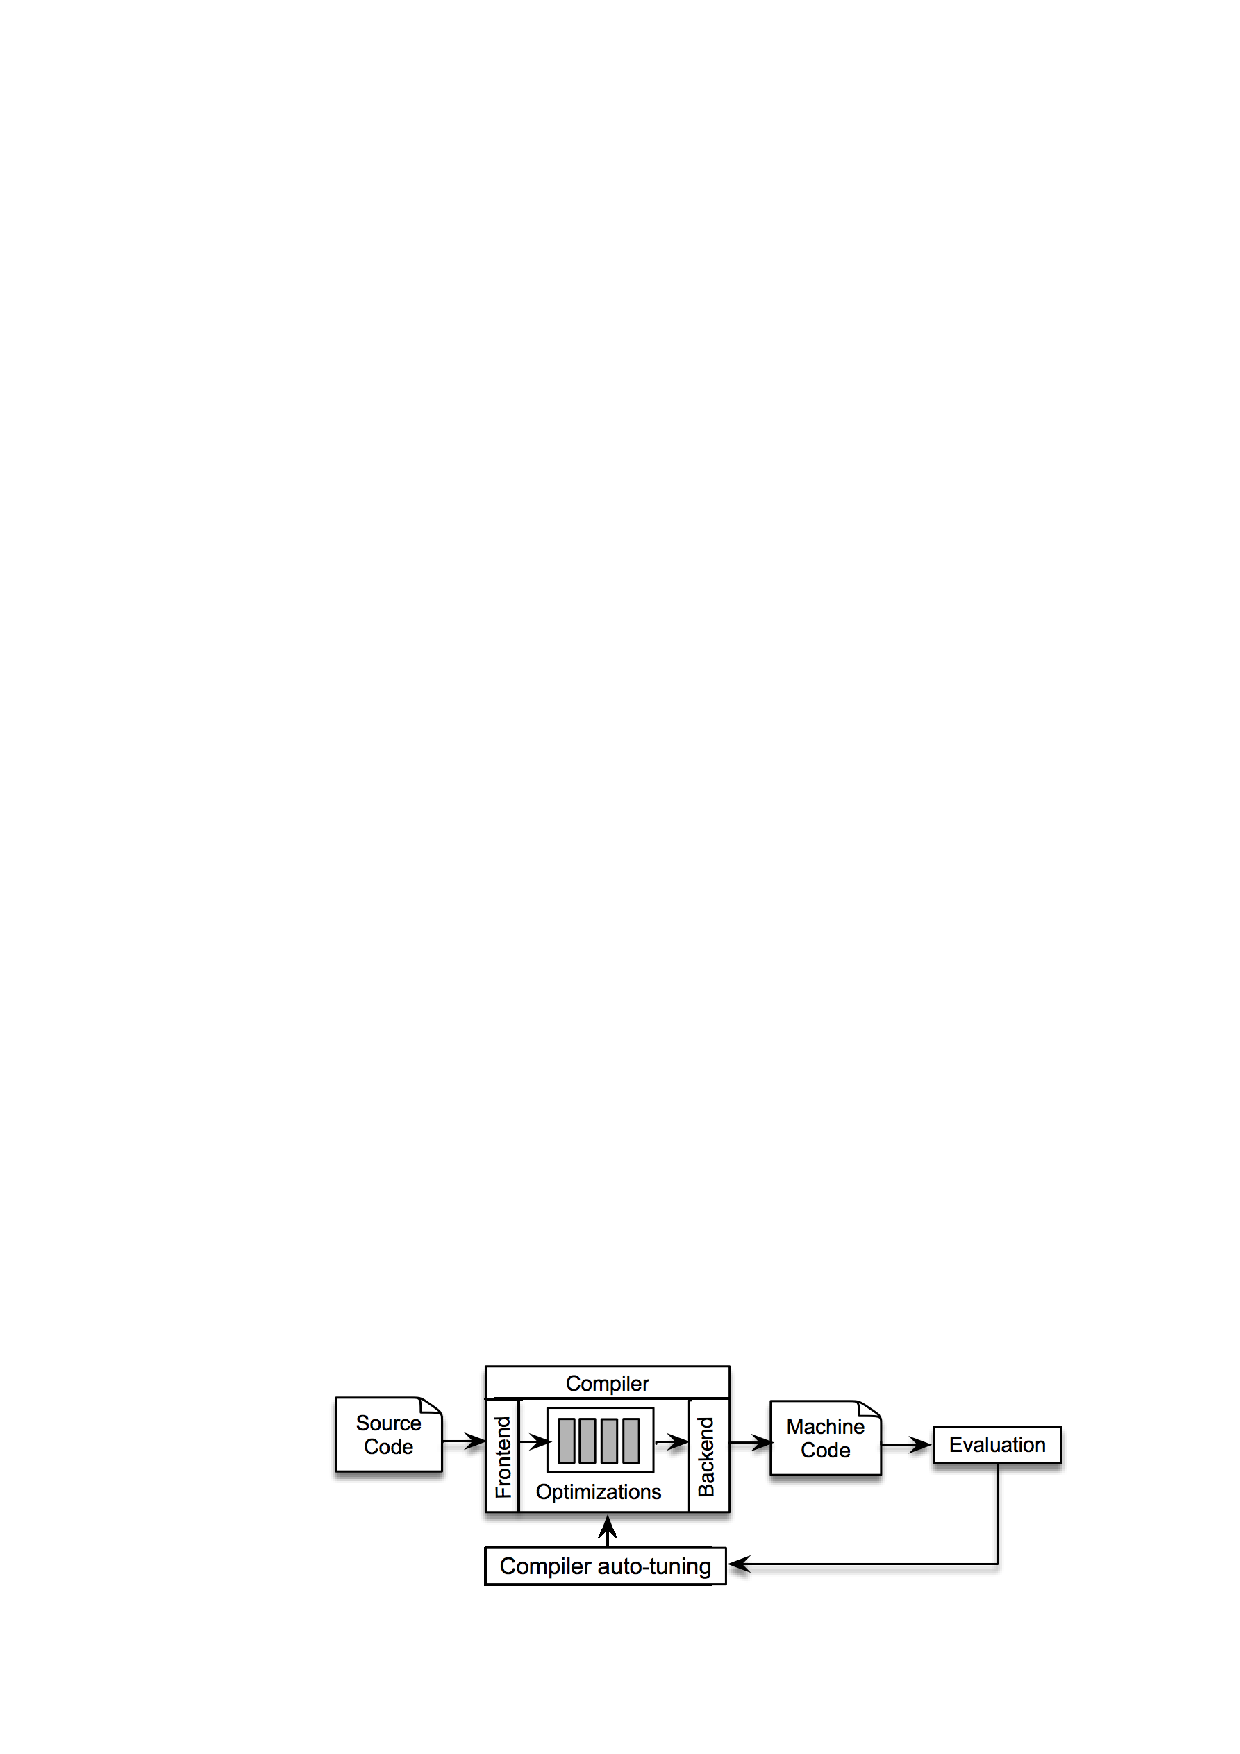
\includegraphics[width=0.9\linewidth]{chapitre3/fig/autotuning.pdf}
	\caption{Process of compiler optimization exploration}
	
\end{figure}

\subsection{Example: GCC Compiler}
\begin{figure}[!htbp]
	\centering
	\includegraphics[width=0.9\linewidth]{chapitre3/fig/optimizations.png}
	\caption{Process of compiler optimization exploration}
	
\end{figure}
The GNU Compiler Collection, GCC, is a very popular collection of programming compilers, available for different platforms.
GCC exposes its various optimizations via a number of flags that can be turned on or off through command-line compiler switches. 
% We choose GCC compiler as a motivating example in order to explain how we would study the impact of compiler optimizations using a component-based infrastructure for testing and monitoring.
% In next section, we present a search-based technique called Novelty Search for automatic generation of optimization sequences.

For instance, version 4.8.4 provides a wide range of command-line options that can be enabled or disabled, including more than 150 options for optimization. The diversity of available optimization options makes the design space for optimization level very huge, increasing the need for heuristics to explore the search space of feasible optimization sequences.
For instance, we count 76 optimization flags that are enabled by the four default optimization levels (O1, O2, O3, Ofast). 
In fact, O1 reduces the code size and execution time without performing any optimization that reduces the compilation time. It turns on 32 flags. 
O2 increases the compilation time and reduces the execution time of generated code. It turns on all optimization flags specified by O1 plus 35 other options. 
O3 is more aggressive level which enables all O2 options plus eight more optimizations. 
Finally, Ofast is the most aggressive level which enables optimizations that are not valid for all standard-compliant programs. It turns on all O3 optimizations plus one more aggressive optimization. 
%For example, in GCC, we can distinguish optimization levels from O1 to O3. Each optimization level involves a fixed list of compiler optimization options
This results in a huge space with $2^{76}$ possible optimization combinations. The full list of optimizations is available here~\cite{mboussaa}.
%In our approach, we did not consider some optimization options that are enabled by default, since they do not affect the performance of generated binaries.
Optimization flags in GCC can be turned off by using \textit{"fno-"}+flag instead of \textit{"f"}+flag in the beginning of each optimization. 
We use this technique to play with compiler switches.

\iffalse
\begin{table}
	\label{table:options}
	\centering
	\caption{Compiler optimization options within standard optimization levels}
	\scalebox{0.88}{
		\begin{tabular}[c]{|c|p{3cm}||c|p{3cm}|}
			
			
			\cline{1-4}
			\textbf{Level} & \textbf{Optimization option} & \textbf{Level} & \textbf{Optimization option}  \\
			\hline
			O1 & 
			-fauto-inc-dec \newline
			-fcompare-elim \newline
			-fcprop-registers \newline
			-fdce \newline
			-fdefer-pop \newline
			-fdelayed-branch \newline
			-fdse \newline
			-fguess-branch-probability \newline
			-fif-conversion2 \newline
			-fif-conversion \newline
			-fipa-pure-const \newline
			-fipa-profile \newline
			-fipa-reference\newline 
			-fmerge-constants\newline 
			-fsplit-wide-types \newline
			-ftree-bit-ccp \newline
			-ftree-builtin-call-dce \newline
			-ftree-ccp \newline
			-ftree-ch \newline
			-ftree-copyrename \newline
			-ftree-dce \newline
			-ftree-dominator-opts \newline
			-ftree-dse \newline
			-ftree-forwprop \newline
			-ftree-fre \newline
			-ftree-phiprop \newline
			-ftree-slsr \newline
			-ftree-sra \newline
			-ftree-pta \newline
			-ftree-ter \newline
			-funit-at-a-time
			
			&
			\multirow{2}{*}{O2} & \multirow{2}{6cm} {
				-fthread-jumps\newline 
				-falign-functions\newline  
				-falign-jumps \newline
				-falign-loops  \newline
				-falign-labels \newline
				-fcaller-saves \newline
				-fcrossjumping \newline
				-fcse-follow-jumps  \newline
				-fcse-skip-blocks \newline
				-fdelete-null-pointer-checks \newline
				-fdevirtualize \newline
				-fexpensive-optimizations \newline
				-fgcse  \newline
				-fgcse-lm  \newline
				-fhoist-adjacent-loads \newline
				-finline-small-functions \newline
				-findirect-inlining \newline
				-fipa-sra \newline
				-foptimize-sibling-calls \newline
				-fpartial-inlining \newline
				-fpeephole2 \newline
				-fregmove \newline
				-freorder-blocks  \newline
				-freorder-functions \newline
				-frerun-cse-after-loop \newline 
				-fsched-interblock \newline 
				-fsched-spec \newline
				-fschedule-insns  \newline
				-fschedule-insns2 \newline
				-fstrict-aliasing \newline
				-fstrict-overflow \newline
				-ftree-switch-conversion\newline -ftree-tail-merge \newline
				-ftree-pre \newline
				-ftree-vrp
			} \\
			\cline{1-2}
			O3 & 
			-finline-functions \newline
			-funswitch-loops\newline
			-fpredictive-commoning \newline
			-fgcse-after-reload \newline
			-ftree-vectorize \newline
			-fvect-cost-model \newline
			-ftree-partial-pre \newline 
			-fipa-cp-clone  & &  \\
			\cline{1-2}
			Ofast & -ffast-math &   &  \\
			\hline
			
		\end{tabular}
	}
\end{table}
\fi

\section{Evolutionary Exploration of Compiler Optimizations }


Many techniques (meta-heuristics, constraint programming, etc.) can be used to explore the large set of optimization combinations of modern compilers. 
In our approach, we study the use of the Novelty Search (NS) technique to identify the set of compiler optimization options that optimize the non-functional properties of code.

\subsection{Novelty Search Adaptation}
%Optimization options are difficult and even impossible to be chosen by programmers or compiler users.
%Therefore, a tool to help users to choose the best set of options becomes necessary to achieve a compiler optimization with effectiveness.

In this work, we aim at providing a new alternative for choosing effective compiler optimization options compared to the state of the art approaches. 
In fact, since the search space of possible combinations is too large, we aim at using a new search-based technique called Novelty Search~\cite{lehman2008exploiting} to tackle this issue. 
The idea of this technique is to explore the search space of possible compiler flag options by considering sequence diversity as a single objective. 
Instead of having a fitness-based selection that maximizes one of the non-functional objectives, we select optimization sequences based on a novelty score showing how different they are compared to all other combinations evaluated so far. 
We claim that the search towards effective optimization sequences is not straightforward since the interactions between optimizations is too complex and difficult to define. 
For instance, in a previous work~\cite{chen2012deconstructing}, Chen et al. showed that handful optimizations may lead to higher performance than other techniques of iterative optimization. 
In fact, the fitness-based search may be trapped into some local optima that cannot escape. 
This phenomenon is known as \textit{"diversity loss"}. For example, if the most effective optimization sequence that induces less execution time lies far from the search space defined by the gradient of the fitness function, then some promising search areas may not be reached. 
The issue of premature convergence to local optima has been a common problem in evolutionary algorithms. 
Many methods are proposed to overcome this problem~\cite{banzhaf1996effect}. 
However, all these efforts use a fitness-based selection to guide the search. Considering diversity as the unique objective function to be optimized may be a key solution to this problem.
Therefore, during the evolutionary process, we select optimization sequences that remain in sparse regions of the search space in order to guide the search towards novelty. 
In the meantime, we choose to gather non-functional metrics of explored sequences such as memory consumption. 
We describe in more details the way we are collecting these non-functional metrics in section 4.

Generally, NS acts like GAs (Example of GA use in  \cite{cooper2002adaptive}). However, NS needs extra changes. First, a new novelty metric is required to replace the fitness function. Then, an archive must be added to the algorithm, which is a kind of a database that remembers individuals that were highly novel when they were discovered in past generations. 
Algorithm~\ref{algo:search} describes the overall idea of our NS adaptation. The algorithm takes as input a source code program and a list of optimizations. We initialize first the novelty parameters and create a new archive with limit size L (lines 1 \& 2). In this example, we gather information about memory consumption. In lines 3 \& 4, we compile and execute the input program without any optimization (O0). Then, we measure the resulting memory consumption. By doing so, we will be able to compare it to the memory consumption of new generated solutions. The best solution is the one that yields to the lowest memory consumption compared to O0 usage.
Before starting the evolutionary process, we generate an initial population with random sequences. Line 6-21 encode the main NS loop, which searches for the best sequence in terms of memory consumption. For each sequence in the population, we compile the input program, execute it and evaluate the solution by calculating the average distance from its k-nearest neighbors. Sequences that get a novelty metric higher than the novelty threshold T are added to the archive. T defines the threshold for how novel a sequence has to be before it is added to the archive. In the meantime, we check if the optimization sequence yields to the lowest memory consumption so that, we can consider it as the best solution. Finally, genetic operators
(mutation and crossover) are applied afterwards to fulfill the next population. This process is iterated until reaching the maximum number of evaluations.


\begin{algorithm}
	\algsetup{linenosize=\tiny}
	\footnotesize
	%footnotesize
	\caption{Novelty search algorithm for compiler optimization exploration}
	\label{algo:search}
	\begin{algorithmic}[1]
		
		\REQUIRE Optimization options $\mathcal{O}$
		\REQUIRE Program $\mathcal{C}$
		\REQUIRE Novelty threshold $\mathcal{T}$
		\REQUIRE Limit $\mathcal{L}$
		\REQUIRE Nearest neighbors $\mathcal{K}$
		\REQUIRE Number of evaluations $\mathcal{N}$
		\ENSURE Best optimization sequence $best\_sequence$
		\STATE $initialize\_parameters(\mathcal{L},\mathcal{T},\mathcal{N},\mathcal{K})$
		\STATE $create\_archive(\mathcal{L})$
		\STATE 	$generated\_code \gets compile(\textit{"-O0"},\mathcal{C})$
		\STATE 	$minimum\_usage \gets execute(generated\_code)$
		\STATE $population \gets random\_sequences(\mathcal{O})$
		\REPEAT
		\FOR{$sequence \in population$}   
		\STATE 	$generated\_code \gets compile(sequence,\mathcal{C})$
		\STATE 	$memory\_usage \gets execute(generated\_code)$
		\STATE	$novelty\_metric(sequence) \gets distFromKnearest(archive,population,\mathcal{K})$
		\IF{$novelty\_metric > \mathcal{T}$}
		\STATE	$archive \gets archive \cup sequence$
		\ENDIF
		
		\IF{$memory\_usage < minimum\_usage$}
		\STATE	$best\_sequence \gets sequence$
		\STATE	$minimum\_usage \gets memory\_usage$
		\ENDIF
		
		\ENDFOR
		\STATE		$new\_population \gets generate\_new\_population(population)$
		\STATE		$generation \gets generation + 1$
		\UNTIL{$generation = \mathcal{N}$}
		\RETURN $best\_sequence$
	\end{algorithmic}
\end{algorithm}


\subsubsection{Optimization Sequence Representation}
For our case study, a candidate solution represents all compiler switches that are used in the four standard optimization levels (O1, O2, O3 and Ofast). Thereby, we represent this solution as a vector where each dimension is a compiler flag. 
The variables that represent compiler options are represented as genes in a chromosome. 
Thus, a solution represents the CFLAGS value used by GCC to compile programs.
A solution has always the same size, which corresponds to the total number of involved flags. 
However, during the evolutionary process, these flags are turned on or off depending on the mutation and crossover operators (see example in Figure 2). As well, we keep the same order of invoking compiler flags since that does not affect the optimization process and it is handled internally by GCC.
\begin{figure}[h]
	\centering
	\includegraphics[width=1\hsize]{chapitre3/fig/individual.png}
	\caption{Solution representation}
	
\end{figure}

\subsubsection{Novelty Metric}
The Novelty metric expresses the sparseness of an input optimization sequence. It measures its distance to all other sequences in the current population and to all sequences that were discovered in the past (\ie, sequences in the archive). 
We can quantify the sparseness of a solution as the average distance to the k-nearest neighbors. 
If the average distance to a given point's nearest neighbors is large then it belongs to a sparse area and will get a high novelty score. 
Otherwise, if the average distance is small so it belongs certainly to a dense region then it will get a low novelty score. 
The distance between two sequences is computed as the total number of symmetric differences among optimization sequences. Formally, we define this distance as follows :
\begin{equation}
distance(S1,S2)=\left | S1 \bigtriangleup S2 \right |
\end{equation}
where $S1$ and $S2$ are two selected optimization sequences (solutions). The distance value is equal to 0 if the two optimization sequences are similar and higher than 0 if there is at least one optimization difference. The maximum distance value is equal to the total number of input flags.

To measure the sparseness of a solution, we use the previously defined distance to compute the average distance of a sequence to its k-nearest neighbors. In this context, we define the novelty metric of a particular solution as follows:
\begin{equation}
NM(S) = \frac{1}{k} \sum_{i=1}^{k} distance(S,\mu _{i})
\end{equation}
where $\mu _{i}$ is the $i^{th}$ nearest neighbor of the solution S within the population and the archive of novel individuals. 

\subsection{Novelty Search For Multi-objective Optimization}
A multi-objective approach provides a trade-off between two objectives where the developers can select their desired solution from the Pareto-optimal front. The idea of this approach is to use multi-objective algorithms to find trade-offs between non-functional properties of generated code such as \textit{$<$ExecutionTime--MemoryUsage$>$}. The correlations we are trying to investigate are more related to the trade-offs between resource consumption and execution time.

For instance, NS can be easily adapted to multi-objective problems. In this adaptation, the SBSE formulation remains the same as described in Algorithm 1. However, in order to evaluate the new discovered solutions, we have to consider two main objectives and add the non-dominated solutions to the Pareto non-dominated set. We apply the Pareto dominance relation to find solutions that are not Pareto dominated by any other solution discovered so far, like in NSGA-II~\cite{lokuciejewski2010multi, deb2002fast}. Then, this Pareto non-dominated set is returned as a result.
There is typically more than one optimal solution at the end of NS. The maximum size of the final Pareto set cannot exceed the size of the initial population.


\section{Evaluation}
So far, we have presented a sound procedure and automated component-based framework for extracting the non-functional properties of generated code. In this section, we evaluate the implementation of our approach by explaining the design of our empirical study; the research questions we set out to answer and different methods we used to answer these questions. The experimental material is available for replication purposes\footnote{https://noticegcc.wordpress.com/}.

\subsection{Research Questions}
Our experiments aim at answering the following research questions:

\textbf{RQ1: Mono-objective SBSE Validation.} 
\textit{How does the proposed diversity-based exploration of optimization sequences perform compared to other mono-objective algorithms in terms of memory and CPU consumption, execution time, etc.?} 


\textbf{RQ2: Sensitivity.} 
\textit{How sensitive are input programs to compiler optimization options?}


\textbf{RQ3: Impact of optimizations on resource consumption.} 
\textit{How compiler optimizations impact on the non-functional properties of generated programs?}


\textbf{RQ4: Trade-offs between non-functional properties.} 
\textit{How can multi-objective approaches be useful to find trade-offs between non-functional properties?}

To answer these questions, we conduct several experiments using NOTICE to validate our global approach for non-functional testing of compilers using system containers.


\subsection{Experimental Setup}
\subsubsection{Programs Used in the Empirical Study}
To explore the impact of compiler optimizations a set of input programs are needed. 
To this end, we use a random C program generator called Csmith~\cite{yang2011finding}.
Csmith is a tool that can generate random C programs that statically and dynamically conform to the C99 standard. It has been widely used to perform functional testing of compilers~\cite{chen2016empirical,le2014compiler,nagai2013scaling} but not the case for checking non-functional requirements. Csmith can generate C programs that use a much wider range of C features including complex control flow and data structures such as pointers, arrays, and structs. Csmith programs come with their test suites that explore the structure of generated programs. 
Authors argue that Csmith is an effective bug-finding tool because it generates tests that explore atypical combinations of C language features. They also argue that larger programs are more effective for functional testing. Thus, we run Csmith for 24 hours and gathered the largest generated programs. We depicted 111 C programs with an average number of source lines of 12K. 10 programs are used as training set for RQ1, 100 other programs to answer RQ2 and one last program to run RQ4 experiment.
Selected Csmith programs are described in more details at~\cite{mboussaa}.
%Moreover, we run experiments on commonly used benchmarks in iterative compilation named Collective Benchmark (Cbench)~\cite{fursin2009collective}. It is a collection of open-source sequential programs in C, targeting specific areas of the embedded market. It comes with multiple datasets assembled by the community to enable realistic benchmarking and research on program and architecture optimization. Cbench contains more than 20 C programs. 

\iffalse
\begin{table}[h]
	\begin{center}
		\begin{tabular}{|c|c|p{3.9cm}|}
			\hline
			\textbf{Program} & \textbf{Source lines} & \textbf{Description}\\
			\hline
			automative\_susan\_s & 1376 & Image recognition package\\
			\hline
			bzip2e & 5125 & Compress any file
			source code \\
			\hline
			bzip2d & 5125 & Decompress zipped files \\
			\hline
			office\_rsynth & 4111 & Text to speech program produced by integrating various pieces of code\\
			\hline
			consumer\_tiffmedian& 15870 & Apply the median cut algorithm to data in a TIFF file
			\\
			
			\hline
			consumer\_tiffdither& 15399 & Convert a greyscale image to bilevel using dithering
			\\
			\hline
			
		\end{tabular}
		
	\end{center}
	\caption {Description of selected benchmark programs}
\end{table}
\fi
\subsubsection{Parameters Tuning}
%Our experiments use the classical NS algorithm, where we evolve a set of optimization sequences through generations.
An important aspect for meta-heuristic search algorithms lies in the parameters tuning and selection, which are necessary to ensure not only fair comparison, but also for potential replication.
NOTICE implements three mono-objective search algorithms (Random Search (RS), NS, and GA~\cite{cooper2002adaptive}) and two multi-objective optimizations (NS and NSGA-II~\cite{deb2002fast}). Each initial population/solution of different algorithms is completely random. The stopping criterion is when the maximum number of fitness evaluations is reached.
The resulting parameter values are listed in Table 2. The same parameter settings are applied to all algorithms under comparison.

NS, which is our main concern in this work, is implemented as described in Section 3. During the evolutionary process, each solution is evaluated using the novelty metric. Novelty is calculated for each solution by taking the mean of its 15 nearest optimization sequences in terms of similarity (considering all sequences in the current population and in the archive). Initially, the archive is empty. Novelty distance is normalized in the range [0-100].
Then, to create next populations, an elite of the 10 most novel organisms is copied unchanged, after which the rest of the new population is created by tournament selection according to novelty (tournament size = 2). Standard genetic programming crossover and mutation operators are applied to these novel sequences in order to produce offspring individuals and fulfill the next population (crossover = 0.5, mutation = 0.1).
In the meantime, individuals that get a score higher than 30 (threshold T), they are automatically added to the archive as well. 
In fact, this threshold is dynamic. Every 200 evaluations, we check how many individuals have been copied into the archive. If this number is below 3, the threshold is increased by multiplying it by 0.95, whereas if solutions added to archive are above 3, the threshold is decreased by multiplying it by 1.05. 
Moreover, as the size of the archive grows, the nearest-neighbor calculation that determines the novelty scores for individuals becomes more computationally demanding. So, to avoid having low accuracy of novelty, we choose to limit the size of the archive (archive size = 500). Hence, it follows a first-in first-out data structure which means that when a new solution gets added, the oldest solution in the novelty archive will be discarded. Thus, we ensure individual diversity by removing old sequences that may no longer be reachable from the current population.

Algorithm parameters were tuned individually in preliminary experiments. For each parameter, a set of values was tested. The parameter values chosen are the mostly used in the literature~\cite{inden2013examination}. The value that yielded the highest performance score was chosen.  

\begin{table}
	\caption{Algorithm parameters}
	\begin{tabular}{| l |l| l |l| }\hline
		\textbf{Parameter} & \textbf{Value} & \textbf{Parameter} & \textbf{Value} \\	\hhline{|=|=|=|=|}	
		Novelty nearest-k  & 15 &  Tournament size & 2\\ 
		Novelty threshold & 30 &  Mutation prob. & 0.1\\  
		Max archive size & 500 &  Crossover & 0.5  \\  
		Population size & 50 &  Nb generations &  100 \\  
		Individual length & 76 & Elitism & 10  \\ 
		Scaling archive prob. & 0.05 & Solutions added to archive & 3  \\ 	\hline
	\end{tabular}
\end{table}
\setlength{\textfloatsep}{2pt}
\subsubsection{Evaluation Metrics Used}

For mono-objective algorithms, we use to evaluate solutions using the following metrics:

-\textit{Memory Consumption Reduction (MR)}: corresponds to the percentage ratio of memory usage reduction of running container over the baseline. The baseline in our experiments is O0 level, which means a non-optimized code. Larger values for this metric mean better performance. Memory usage is measured in bytes.

-\textit{CPU Consumption Reduction (CR)}: corresponds to the percentage ratio of CPU usage reduction over the baseline. Larger values for this metric mean better performance. The CPU consumption is measured in seconds, as the CPU time.

-\textit{Speedup (S)}: corresponds to the percentage improvement in execution speed of an optimized code compared to the execution time of the baseline version. Program execution time is measured in seconds.


%When comparing two mono-objective algorithms, it is usual to compare their best solutions found so far during the optimization process. However, this is not applicable when comparing two multi-objective evolutionary algorithms since each of them gives as output a set of non-dominated (Pareto equivalent) solutions. For this reason, we use performance indicator to compare multi-objective algorithms.
%Thus, for multi-objective algorithms we use to evaluate solutions using the following metric:

%-\textit{Hypervolume (HV)}: corresponds to the proportion of objective space that is dominated by the Pareto front approximation returned by the algorithm and delimited by a reference point. The HV reference point is the point obtained by taking the maximum value observed. Thus, the HV metric can be computed as the area between the Pareto frontier and the HV reference point. Larger values for this metric mean better performance. The most interesting features of this indicator are its Pareto dominance compliance and its ability to capture both convergence and diversity~\cite{deb2001multi}. 

\subsubsection{Setting up Infrastructure}
To answer the previous research questions, we configure NOTICE to run different experiments. Figure 4 shows a big picture of the testing and monitoring infrastructure considered in these experiments. 
First, a meta-heuristic (mono or multi-objective) is applied to generate specific optimization sequences for the GCC compiler (step 1). During all experiments, we use GCC 4.8.4, as it is introduced in the motivation section, although it is possible to choose another compiler version using NOTICE since the process of optimizations extraction is done automatically. 
Then, we generate a new optimized code and deploy the output binary within a new instance of our preconfigured Docker image (step 2). While executing the optimized code inside the container, we collect runtime performance data (step 4) and record it in a new time-series database using our InfluxDB back-end container (step 5). Next, NOTICE accesses remotely to stored data in InfluxDB using REST API calls and assigns new performance values to the current solution (step 6). The choice of performance metrics depends on experiment objectives (Memory improvement, speedup, etc.).
\begin{figure}[h]
	\centering
	\includegraphics[width=0.8\linewidth]{chapitre3/fig/infraup.pdf}
	\caption{NOTICE experimental infrastructure}
\end{figure}

To obtain comparable and reproducible results, we use the same hardware across all experiments: an AMD A10-7700K APU Radeon(TM) R7 Graphics processor with 4 CPU cores (2.0 GHz), running Linux with a 64 bit kernel and 16 GB of system memory.

\subsubsection{Tool Support}		
NOTICE is also a GUI framework. It provides different features for non-functional testing of compilers.

For instance, compiler users can:
\begin{itemize} 
	
	
	\item define input program under test: generate Csmith program or use Cbench benchmark programs
	\item define datasets: select dataset for selected program
	\item select target system architecture: choose processor architecture such as x64, x86, ARM. This is part of our future work since we are running experiments only on a x64 architecture. We are preparing a QEMU docker image to handle platforms heterogeneity.
	\item define compiler versions: GCC compiler version from 3.x to 5.x
	\item configure monitoring components: versions, labels, ports, logins, passwords
	\item choose ip address of cloud host machine where experiments will be running
	\item define resource constraints to running container: in case we would run optimizations under resource constraints.
	\item choose search method: mono or multi-objective search
	\item choose meta-heuristic algorithm: GA, RS, NS, NSGA-II
	\item choose the number of iterations: number of evaluations
	\item choose optimization goal: the goal can be execution time, memory, cpu, code size or compilation time optimizations. For multi objective search, users can choose trade-offs between these objectives.
\end{itemize} 
\begin{figure}[h]
	\center
	\includegraphics[scale=0.65]{chapitre3/fig/tool_support}
	\caption{Snapshot of NOTICE GUI interface}
	\label{fig:tool_support}
\end{figure}
The execution result of this tool will be the best optimization sequences corresponding to user requirements.

\subsection{Experimental Methodology and Results}
In the following paragraphs, we report the methodology and results of our experiments.

\subsubsection{RQ1. Mono-objective SBSE Validation}
\paragraph{Method}

To answer the first research question RQ1, we conduct a mono-objective search for compiler optimization exploration in order to evaluate the non-functional properties of optimized code. Thus, we generate optimization sequences using three search-based techniques (RS, GA, and NS) and compare their performance results to standard GCC optimization levels (O1, O2, O3, and Ofast). 
In this experiment, we choose to optimize for execution time (S), memory usage (MR), and CPU consumption (CR). Each non-functional property is improved separately and independently of other metrics. We recall that other properties can be also optimized using NOTICE (e.g., code size, compilation time, etc.), but in this experiment, we focus only on three properties.
\vspace{-1em}
\begin{figure}[h]
	\centering
	\includegraphics[width=1.\linewidth]{chapitre3/fig/sensitivity.pdf}
	\caption{Evaluation strategy to answer RQ1 and RQ2}
	
\end{figure}

\setlength\abovecaptionskip{0.25ex}
As it is shown on the left side of Figure 5, given a list of optimizations and a non-functional objective, we use NOTICE to search for the best optimization sequence across a set of input programs that we call \textit{"the training set"}. This \textit{"training set"} is composed of random Csmith programs (10 programs). We apply then generated sequences to these programs. Therefore, the code quality metric, in this setting, is equal to the average performance improvement (S, MR, or CR) and that, for all programs under test. 

%while p
%the goal of this initial experiment is to: (1) evaluate the effectiveness of our component-based infrastructure to extract non-functional properties such as memory and CPU consumptions; (2) evaluate the performance of our proposed diversity-based exploration of optimization sequences (NS) to GA and RS; and finally (3) find the optimal solution relative to the input training set.

%The goal of this experiment is to show that NOTICE is able to generate 





\paragraph{Results}


\vspace{-1.2em}
%\iffalse
\begin{table}[h]
	\centering
	\caption{Results of mono-objective optimizations}
	\label{my-label}
	\begin{tabular}{|l|l|l|l|l|l|l|c|}
		\hline
		& \textbf{O1}                    & \textbf{O2}                    & \textbf{O3}                    & \textbf{Ofast}                 & \textbf{RS}                    & \textbf{GA}                    & 
		\textbf{NS} \\
		\hhline{|=|=|=|=|=|=|=|=|}
		S  &  1.051 & 1.107  & 1.107  & 1.103  & 1.121  &  1.143 &  1.365  \\ \hline
		MR(\%) & 4.8  & -8.4  &  4.2 & 6.1  &  10.70 & 15.2  &  15.6  \\ \hline
		CR(\%) & -1.3  & -5  & 3.4  & -5  &  18.2 & 22.2  &  23.5  \\ \hline
	\end{tabular}
\end{table}
%\fi
%-NS better than 3 algos\\
%-conflicting results for standard levels
%The goal of this first experiment is to compare the performance improvement of novelty-based generated sequences to standard GCC optimizations and to RS and GA.  
Table 3 reports the comparison results of three non-functional properties CR, MR, and S. At the first glance, we can clearly see that all search-based algorithms outperform standard GCC levels with minimum improvement of 10\% for memory usage and 18\% for CPU time (when applying RS). 
Our proposed NS approach has the best improvement results for three metrics with 1.365 of speedup, 15.6\% of memory reduction and 23.5\% of CPU time reduction across all programs under test. NS is clearly better than GA in terms of speedup. However, for MR and CR, NS is slightly better than GA with 0.4\% improvement for MR and 1.3\% for CR. RS has almost the lowest optimization performance but is still better than standard GCC levels.

We remark as well that applying standard optimizations has an impact on the execution time with a speedup of 1.107 for O2 and O3. Ofast has the same impact as O2 and O3 for the execution speed. However, the impact of GCC levels on resource consumption is not always efficient. O2, for example, increases resource consumption compared to O0 (-8.4\% for MR and -5\% for CR). This can be explained by the fact that standard GCC levels apply some aggressive optimizations that increase the performance of generated code and deteriorate system resources.  
%Thus, NOTICE can clearly provide an alternative to catch most relevant optimization sequence regarding resource consumptions.

%This agrees to the idea that standard optimizations mdoes not produce always
%the same impact results on resource consumption and may be highly dependent on the benchmark and the source code they have been tested on.
%Using O2, we find that the memory consumption has increased by almost 8.4\% compared to the baseline. Same findings for CR when applying O1, O2 and Ofast. 



\noindent\fbox{\parbox{\linewidth-2\fboxrule-2\fboxsep}{
		\textbf{Key findings for RQ1.} \\
		-- Best discovered optimization sequences using mono-objective search techniques always provide better results than standard GCC optimization levels.\\
		-- Novelty Search is a good candidate to improve code in terms of non-functional properties since it is able to discover optimization combinations that outperform RS and GA.  }}
\\
\subsubsection{RQ2. Sensitivity}
\paragraph{Method}
Another interesting experiment is to test the sensitivity of input programs to compiler optimizations and evaluate the general applicability of best optimal optimization sets, previously discovered in RQ1. These sequences correspond to the best generated sequences using NS for the three non-functional properties S, MR and CR (i.e., sequences obtained in column 8 of Table 3). 
Thus, we apply best discovered optimizations in RQ1 to new unseen Csmith (100 new random programs) and we compare then, the performance improvement across these programs (see right side of Figure 5). We also apply standard optimizations, O2 and O3, to new Csmith programs in order to compare the performance results.
The idea of this experiment is to test whether new generated Csmith programs are sensitive to previously discovered optimizations or not. 
%If so, then compiler users and researchers can use NOTICE to auto-tune compilers and build optimizations for their input programs. 
%in order to build general optimization sequences from their representative
If so, this will be useful for compiler users and researchers to use NOTICE in order to build general optimization sequences from their representative \textit{training set} programs.
\vspace{-1.2em}
\begin{figure}[h]
	\centering
	\includegraphics[width=1.\linewidth]{chapitre3/fig/box.pdf}
	\caption{Boxplots of the obtained performance results across 100 unseen Csmith programs, for each non-functional property: Speedup (S), memory (MR) and CPU (CR) and for each optimization strategy: O2, O3 and NS}
\end{figure}
\paragraph{Results}
Figure 6 shows the distribution of memory, CPU and speedup improvement across new Csmith programs. For each non-functional property, we apply O2, O3 and best NS sequences. Speedup results show that the three optimization strategies lead to almost the same distribution with a median value of 1.12 for speedup. This can be explained by the fact that NS might need more time to find the sequence that best optimizes the execution speed. Meanwhile, O2 and O3 have also the same impact on CR and MR which is almost the same for both levels (CR median value is 8\% and around 5\% for MR).
However, the impact of applying best generated sequences using NS clearly outperforms O2 and O3 with almost 10\% of CPU improvement and 7\% of memory improvement. This proves that NS sequences are efficient and can be used to optimize resource consumption of new Csmith programs. This result also proves that Csmith code generator applies the same rules and structures to generate C code. For this reason, applied optimization sequences always have a positive impact on the non-functional properties.


\noindent\fbox{\parbox{\linewidth-2\fboxrule-2\fboxsep}{
		\textbf{Key findings for RQ2.}\\
		-- It is possible to build general optimization sequences that perform better than standard optimization levels \\
		-- Best discovered sequences in RQ1 can be mostly used to improve the memory and CPU consumption of Csmith programs. To answer RQ2, Csmith programs are sensitive to compiler optimizations.}}\\
\subsubsection{RQ3. Impact of optimizations on resource usage}
\paragraph{Method}
In this experiment, we use NOTICE to provide an understanding of optimizations behavior, in terms of resource consumption, when trying to optimize for execution time. Thus, we choose one instance of obtained results in RQ1 related to the best speedup improvement (i.e., results obtained in line 1 of Table 3) and we study the impact of speedup improvement on memory and CPU consumption. We also compare resource usage data to standard GCC levels as they were presented in Table 3. Improvements are always calculated over the non-optimized version. The idea of this experiment is to: (1) prove, or not, the usefulness of involving resource usage metrics as key objectives for performance improvement; (2) the need, or not, of multi-objective search strategy to handle both resource usage and performance properties.

%In this experiment, we apply standard optimizations and different mono-objective heuristics individually to 5 Cbench programs and use NOTICE to profile applications in terms of resource usage.  

%To answer RQ3, we choose one instance of obtained results in RQ1 related to the best improvement in terms of execution time (i.e., where NS had the best speedup) and we study the impact of performance improvement on memory and CPU consumption. 
%Following again a mono-objective approach, we try in this experiment to maximize the speedup \textit{S} per-benchmark and study, at the same time, the impact of speedup \textit{S} on resource consumption namely memory footprint and CPU usage. 
%In this experiment, we apply standard optimizations and different mono-objective heuristics individually to 5 Cbench programs and use NOTICE to profile applications in terms of resource usage.   
%The goal of this experiment is to: (1) use NOTICE infrastructure to provide an understanding of optimizations behavior, in terms of resource consumption, when trying to optimize for execution time; (2) prove the usefulness of resource consumption reduction as a key objective for performance improvement.

\paragraph{Results}

%\begin{figure}[h]
%	\centering
%	\includegraphics[width=1.\linewidth]{Ressources/infra_novelty_stat2.png}
%	\caption{Evaluating the speedup after applying standard optimization options compared to best generated optimization using NS}
%\end{figure}
Figure 7 shows the impact of speedup optimization on resource consumption. For instance, O2 and O3 that led to the best speedup improvement among standard optimization levels in RQ1, present opposite impact on resource usage. Applying O2 induces -8.4\% of MR and -5\% of CR. However, applying O3 improves MR and CR respectively by 3.4\% and 4.2\%. Hence, we note that when applying standard levels, there is no clear correlation between speedup and resource usage since compiler optimizations are generally used to optimize the execution speed and never evaluated to reduce system resources.
On the other hand, the outcome of applying different mono-objective algorithms for speedup optimization also proves that resource consumption is always in conflict with execution speed. The highest MR and CR is reached using NS with respectively 1.2\% and 5.4\%. This improvement is considerably low compared to scores reached when we have applied resource usage metrics as key objectives in RQ1 (i.e., 15.6\% for MR and 23.5\% for CR). Furthermore, we note that generated sequences using RS and GA have a high impact on system resources since all resource usage values are worse than the baseline.
These results agree to the idea that compiler optimizations do not put too much emphasis on the trade-off between execution time and resource consumption.

%Thus, NOTICE can clearly provide an alternative to catch most relevant optimization sequence regarding resource consumptions.

%This agrees to the idea that standard optimizations mdoes not produce always
%the same impact results on resource consumption and may be highly dependent on the benchmark and the source code they have been tested on.
%Using O2, we find that the memory consumption has increased by almost 8.4\% compared to the baseline. Same findings for CR when applying O1, O2 and Ofast. 
\noindent\fbox{\parbox{\linewidth-2\fboxrule-2\fboxsep}{
		\textbf{Key findings for RQ3.} \\
		-- Optimizing software performance can induce undesirable effects on system resources.\\
		-- A trade-off is needed to find a correlation between software performance and resource usage.
	}}
	
	\subsubsection{RQ4. Trade-offs between non-functional properties}
	\paragraph{Method}
	Finally, to answer RQ4, we use NOTICE again to find trade-offs between non-functional properties. In this experiment, we choose to focus on the trade-off \textit{$<$ExecutionTime--MemoryUsage$>$}. In addition to our NS adaptation for multi-objective optimization, we implement a commonly used multi-objective approach namely NSGA-II~\cite{deb2002fast}. We denote our NS adaptation by \textit{NS-II}. We recall that NS-II is not a multi-objective approach as NSGA-II. It uses the same NS algorithm. However, in this experiment, it returns the optimal Pareto front solutions instead of returning one optimal solution relative to one goal. 
	\begin{figure}[h]
		\centering
		\includegraphics[width=0.9\linewidth]{chapitre3/fig/rq3.pdf}
		\caption{Impact of speedup improvement on memory and CPU consumption for each optimization strategy}
	\end{figure}
	Apart from that, we apply different optimization strategies to assess our approach. 
	
	First, we apply standard GCC levels. Second, we apply best generated sequences relative to memory and speedup optimization (the same sequences that we have used in RQ2). Thus, we denote by \textit{NS-MR} the sequence that yields to the best memory improvement MR and \textit{NS-S} to the sequence that leads to the best speedup. This is useful to compare mono-objective solutions to new generated ones.
	
	
	
	In this experiment, we assess the efficiency of generated sequences using only one Csmith program.
	We evaluate the quality of the obtained Pareto optimal optimization based on raw data values of memory and execution time. Then, we compare qualitatively the results by visual inspection of the Pareto frontiers.
	The goal of this experiment is to check whether it exists, or not, a sequence that can reduce both execution time and memory usage.
	%We report the comparison results of our NS adaptation for optimizations generation to the current state-of-the-art multi-objective approaches namely NSGA-II. 
	
	%Two tradeoffs are investigated in this section; $<$execution time--memory usage$>$ and $<$execution time--CPU usage$>$.
	
	
	\paragraph{Results}
	Figure 8 shows the Pareto optimal solutions that achieved the best performance assessment for the trade-off \textit{$<$ExecutionTime--MemoryUsage$>$}. The horizontal axis indicates the memory usage in raw data (in Bytes) as it is collected using NOTICE. In similar fashion, the vertical axis shows the execution time in seconds. Furthermore, the figure shows the impact of applying standard GCC options and best NS sequences on memory and execution time. Based on these results, we can see that NSGA-II performs better than NS-II. In fact, NSGA-II yields to the best set of solutions that presents the optimal trade-off between the two objectives. Then, it is up to the compiler user to use one solution from this Pareto front that satisfies his non-functional requirements (six solutions for NSGA-II and five for NS-II). For example, he could choose one solution that maximizes the execution speed in favor of memory reduction. On the other side, NS-II is capable to generate only one non-dominated solution. For NS-MR, it reduces as expected the memory consumption compared to other optimization levels. The same effect on execution time when applying the best speedup sequence NS-S. We also note that all standard GCC levels are dominated by our different heuristics NS-II, NSGA-II, NS-S and NS-MR.
	This agrees to the claim that standard compiler levels do not present a suitable trade-off between execution time and memory usage.
	
	
	\begin{figure}[h]
		\centering
		\includegraphics[width=0.9\linewidth]{chapitre3/fig/pareto.pdf}
		\caption{Comparison results of obtained Pareto fronts using NSGA-II and NS-II}
	\end{figure}
	
	
	\noindent\fbox{\parbox{\linewidth-2\fboxrule-2\fboxsep}{
			\textbf{Key findings for RQ4.} \\
			-- NOTICE is able to construct optimization levels that represent optimal trade-offs between non-functional properties. \\
			-- NS is more effective when it is applied for mono-objective search. \\
			-- NSGA-II performs better than our NS adaptation for multi-objective optimization. However, NS-II performs clearly better than standard GCC optimizations and previously discovered sequences in RQ1.
		}}
		\subsection{Discussions}
		Through these experiments, we showed that NOTICE is able to provide facilities to compiler users to test the non-functional properties of generated code. It provides also a support to search for the best optimization sequences through mono-objective and multi-objective search algorithms. NOTICE infrastructure has shown its capability and scalability to satisfy user requirements and key objectives in order to produce efficient code in terms of non-functional properties. During all experiments, standard optimization levels have been fairly outperformed by our different heuristics. 
		Moreover, we have also shown (in RQ1 and RQ3) that optimizing for performance may be, in some cases, greedy in terms of resource usage. For example, the impact of standard optimization levels on resource usage is not always efficient even though it leads to performance improvement. 
		Thus, compiler users would use NOTICE to test the impact of optimizations on the non-functional properties and build their specific sequences by trying to find trade-offs among these non-functional properties (RQ4). We would notice that for RQ1, experiments take about 21 days to run all algorithms. This run time might seem long but, it should be noted that this search can be conducted only once, since in RQ2 we showed that best gathered optimizations can be used with unseen programs of the same category as the training set, used to generate optimizations. This has to be proved with other case studies. As an alternative, it would be great to test model-based code generators. In the same fashion as Csmith, code generators apply to same rules to generate new software programs. Thus, we can use NOTICE to define general-purpose optimizations from a set of generated code artifacts. 
		Multi-objective search as conducted in RQ4, takes about 48 hours, which we believe is acceptable for practical use. Nevertheless, speeding up the search speed may be an interesting feature for future research.
		%good performance to detect most of the existing antipatterns, which
		%could be very helpful to provide advice to both service clients and
		%providers on the quality of their Web services.
		
		
		
		
		%speeding up the search process may be an interesting avenue for future research.
		\subsection{Threats to Validity}
		Any automated approach has limitations. We resume, in the following paragraphs, external and internal threats that can be raised:
		
		\textit{External validity} refers to the generalizability of our findings. In this study, we perform experiments on random programs using Csmith and we use iterative compilation techniques to produce best optimization sequences. We believe that the use of Csmith programs as input programs is very relevant because compilers have been widely tested across Csmith programs~\cite{chen2016empirical,yang2011finding}. Csmith programs have been used only for functional testing, but not for non-functional testing. However, we cannot assert that the best discovered set of optimizations can be generalized to industrial applications since optimizations are highly dependent on input programs and on the target architecture. In fact, experiments conducted on RQ1 and RQ2 should be replicated to other case studies to confirm our findings; and build general optimization sequences from other representative training set programs chosen by compiler users.
		
		\textit{Internal validity} is concerned with the causal relationship between the treatment and the outcome. Meta-heuristic algorithms are stochastic optimizers, they can provide different results for the same problem instance from one run to another. Are we providing a statistically sound method or it is just a random result? Due to time constraints, we run all experiments only once. Following the state-of-the-art approaches in iterative compilation, previous research efforts~\cite{hoste2008cole,martinez2014multi} did not provide statistical tests to prove the effectiveness of their approaches. This is because experiments are time-consuming. However, we can deal with these internal threats to validity by performing at least five independent simulation runs for each problem instance. 
		
		
		\iffalse
		\begin{table}[]
			\centering
			\caption{My caption}
			\label{my-label}
			\begin{tabular}{@{}|l|c|c|c|c|c|c|c|c|c|c|c|c|c|c|c|c|c|c|c|c|@{}}
				\toprule
				\multirow{2}{*}{} & \multicolumn{2}{c|}{CB1} & \multicolumn{2}{c|}{CB2} & \multicolumn{2}{c|}{CB3} & \multicolumn{2}{c|}{CB4} & \multicolumn{2}{c|}{CB5} & \multicolumn{2}{c|}{CS1} & \multicolumn{2}{c|}{CS2} & \multicolumn{2}{c|}{CS3} & \multicolumn{2}{c|}{CS4} & \multicolumn{2}{c|}{CS5} \\ \cmidrule(l){2-21} 
				& Ox & Best & Ox & Best & Ox & Best & Ox & Best & Ox & Best & Ox & Best & Ox & Best & Ox & Best & Ox & Best & Ox & Best \\ \midrule
				Execution Speedup & \begin{tabular}[c]{@{}c@{}}4\%\\ (O3)\end{tabular} &  &  &  &  &  &  &  &  &  &  &  &  &  &  &  &  &  &  &  \\ \midrule
				Memory & \begin{tabular}[c]{@{}c@{}}4\%\\ (O3)\end{tabular} &  &  &  &  &  &  &  &  &  &  &  &  &  &  &  &  &  &  &  \\ \midrule
				CPU & \begin{tabular}[c]{@{}c@{}}4\%\\ (O3)\end{tabular} &  &  &  &  &  &  &  &  &  &  &  &  &  &  &  &  &  &  &  \\ \midrule
				Compilation Speedup &  &  &  &  &  &  &  &  &  &  &  &  &  &  &  &  &  &  &  &  \\ \midrule
				Code Size &  &  &  &  &  &  &  &  &  &  &  &  &  &  &  &  &  &  &  &  \\ \bottomrule
			\end{tabular}
		\end{table}
		\fi
		
		

		
\section{Conclusion and Future Work}
%We present an automated approach for automatic extraction of non-functional properties of generated code.
Modern compilers come with huge number of optimizations, making complicated for compiler users to find best optimization sequences. Furthermore, auto-tuning compilers to meet user requirements is a difficult task since optimizations may depend on different properties (e.g., platform architecture, software programs, target compiler, optimization objective, etc.).
Hence, compiler users merely use standard optimization levels (O1, O2, O3 and Ofast) to enhance the code quality without taking too much care about the impact of optimizations on system resources.

In this chapter, we have introduced first a novel formulation of the compiler optimization problem based on Novelty Search. The idea of this approach is to drive the search for best optimizations toward novelty. Our work presents the first attempt to introduce diversity in iterative compilation. Experiments have shown that Novelty Search can be easily applied to mono and multi-objective search problems. In addition, we have reported the results of an empirical study of our approach compared to different state-of-the-art approaches, and the obtained results have provided evidence to support the claim that Novelty Search is able to generate effective optimizations.
Second, we have presented an automated tool for automatic extraction of non-functional properties of optimized code, called NOTICE. NOTICE applies different heuristics (including Novelty Search) and performs non-functional testing of compilers through the monitoring of generated code in a controlled sand-boxing environment. In fact, NOTICE uses a set of micro-services to provide a fine-grained understanding of optimization effects on resource consumption. 
We evaluated the effectiveness of our approach by verifying the optimizations performed by GCC compiler. 
%Then, we studied the impact of optimizations on memory consumption and execution time across two case studies. 
Results showed that our approach is able to automatically extract information about memory and CPU consumption. We were also able to find better optimization sequences than standard GCC optimization levels.

As a future work, we plan to explore more trade-offs among resource usage metrics \eg, the correlation between CPU consumption and platform architectures. 
We also intend to provide more facilities to NOTICE users in order to test optimizations performed by modern compilers such as Clang, LLVM, etc.
Finally, NOTICE can be easily adapted and integrated to new case studies. As an example, we would inspect the behavior of model-based code generators since different optimizations can be performed to generate code from models~\cite{stuermer2007systematic}. Thus, we aim to use the same approach to find non-functional issues during the code generation process.




\chapter{A lightweight execution environment for automatic software testing and optimization}
\section{Introduction}

Software platforms diversity and hardware heterogeneity, as discussed in Chapter \ref{chap:background}, constitutes a major obstacle for software testing. In fact, running tests requires many environment configurations and settings in order to test the whole application. For example, testing a web application requires the installation of the maven dependencies, web server, libraries, etc. When software developers upgrades the web server version for example, they need to rebuild the application and run the same integration tests in order to check that no errors  have been incorporated. Thus, testing applications using different execution environments and system settings becomes very time consuming and tedious.

For instance, as we discussed in Chapter \ref{chap:code generators} and \ref{chap:compilers}, to evaluate the automatically generated code (by either code generators or compilers), we use to generate code, compile it, and then run test cases. To do so, different system configurations were required to ensure these steps such as installing the generator version (GCC or Haxe versions), install interpreters, compilers, maven dependencies, etc. 

One way to test these configurable generators is to use the virtualization technology. For instance, an alternative method leverages container-based system virtualization (\eg, Docker, as discussed in Section \ref{sec:Lightweight system virtualization for software testing}) to automate the code generation, deployment, and testing inside pre-configured software containers.
This technology enables to mimic the execution environment settings and reproduce the tests in isolated and highly configurable system containers.

When it comes to evaluate the resource consumptions of automatically generated code, this technology becomes very valuable because it allows a fine-grained resource management and isolation. Moreover, it facilitates resource usage extraction and limitation of programs running inside containers. 

This chapter presents a technical description of this lightweight runtime environment and its benefit for automating the non-functional testing of generated code. This infrastructure is used in our two first contributions as means to run tests in a configurable execution environment and to efficiently collect resource consumption metrics.

This chapter is organized as follows: 

Section \ref{mon:System containers} introduces system containers as a lightweight execution environment. We show the benefit of using this technology to automate software testing.

Section \ref{mon:Runtime Testing} describes the runtime monitoring components required to collect resource usage metrics.

Section \ref{mon:case study} shows the adaptation of this sandboxing infrastructure to the generator case study as it is used in Chapters \ref{chap:code generators} and \ref{chap:compilers}.

Finally, we conclude in Section \ref{mon:coclusion}.


\section{System containers as a lightweight execution environment}
\label{mon:System containers}
System containers are operating system-level virtualization method that allows running multiple isolated Linux systems on a control host using a single Linux kernel. 
Containers share the same OS and hardware as the hosting machine and it is very useful to use them in order to create new configurable and isolated instances to run. 
Container-based virtualization reduces the overhead associated with having each guest running a new installed operating system such the case for virtual machines. This approach can also improve the performance because there is just one operating system taking care of hardware calls.
The Linux kernel provides the control groups\footnote{\url{https://fr.wikipedia.org/wiki/Cgroups}} (Cgroups) functionality that allows the limitation and prioritization of resources (CPU, memory, block I/O, network, etc.) inside containers so that, one container does not starve the others in terms of resources.
%Thus, it provides ways to control how much memory, CPU, or block IO a container can use. 

For instance, Docker\footnote{\url{https://www.docker.com}} is a popular container-based technology that automates the deployment of any application as a lightweight, portable, and self-sufficient container, running virtually on a host machine~\cite{merkel2014docker}. 
Today, Docker is one of the most popular infrastructure technology adopted in cloud computing\cite{peinl2016docker}. 
For example, in 2015, Docker had about 3\% market share, and by 2017 it is running on 15\% of the hosts\footnote{\url{https://www.datadoghq.com/docker-adoption/}}.
%To achieve that, Docker uses the Linux container technology. 
Using Docker, it is possible to define pre-configured applications and servers to host as virtual images. It also defines the way the service should be deployed in the host machine using configuration files called Dockerfiles. Moreover, we can enable some configuration options to control and limit resources. For example, we can provide option flags to limit how much memory or CPU usage each service is allowed to consume, associate CPU cores to each service, etc. 


In short, the main advantages of this micro-services approach are:
\begin{itemize}
	\item The use of containers induces less performance overhead compared to using a full stack virtualization solution~\cite{spoiala2016performance}. Indeed, instrumentation and monitoring tools for memory profiling like Valgrind~\cite{nethercote2007valgrind} can induce too much overhead.
	\item Thanks to the use of Dockerfiles, it is possible to easily configure the execution environment in order to build and customize applications using numerous settings (\eg, generator version, dependencies, host IP and OS, optimization options, etc.). Thus, we can use the same configured Docker image to execute different instances of the same application. For hardware architecture, containers share the same platform architecture as the host machine (\eg, x86, x64, ARM, etc.). 
	\item Docker uses Linux control groups (Cgroups) to group processes running in the container. This allows us to manage the resources of a group of processes, which is very valuable. 
	This approach increases the flexibility when we want to manage resources, since we can manage every group individually. For example, if we would evaluate the non-functional requirements of generated code within a resource-constraint environment, we can  request and limit resources within the execution container according to the needs.
	\item Although containers run in isolation, they can share data with the host machine and other running containers. Thus, non-functional data relative to resource consumption can be gathered and managed by other containers (\ie, for storage purpose, visualization)
\end{itemize}

%Thus, instead of configuring all code generators under test (GUTs) within the same host machine, we wrap each GUT within a system container. Afterwards, a new instance of the container is created to enable the execution of generated code in an isolated and configured environment. Meanwhile, we start our runtime testing components. A monitoring component collects usage statistics of all running containers and save them at runtime in a time series database component. Thus, we can compare later information about the resource usage of generated programs and detect inconsistencies within code generators.


%For this purpose, we propose a testing infrastructure based on System Container techniques such as Docker\footnote{\url{https://www.docker.com}} environment. 
%This framework automates the deployment and execution of applications inside software containers by allowing multiple program configurations to run autonomously on different servers (i. e., a cloud servers).
%It also provides a distributed environment where system storage and resources can be finely managed and limited according to the needs. 

%Thus, we integrate a collection of components to define the adequate infrastructure for testing and monitoring of code generators. 






\section{Runtime Monitoring Engine}
\label{mon:Runtime Testing}
In order to monitor the applications (\ie, tests) running within containers, we aim to use a set of Docker components to ease the extraction of resource usage information.


\subsection{Monitoring Container}
First, a monitoring component is needed to collect the resource usage and performance characteristics of running containers. As discussed earlier, Docker relies on Cgroups file systems to expose a lot of metrics about accumulated CPU cycles, memory, block I/O usage, etc. Therefore, our monitoring component automates the extraction of these runtime performance metrics stored in Cgroups files. 
Among the popular ways to do that is to monitor each container via the Docker API, or by installing an agent for detailed visibility inside each container. 
The Docker client already provides a command-line tool to inspect containers' resource consumption. The command \textit{docker stats}, for example, can be used to get the stats about the running containers at runtime. 
If we want to do that manually, we can access to live resource consumption of each container available at the Cgroups file system via stats found in \textit{``/sys/fs/cgroup/cpu/docker/(longid)/''} (for CPU consumption) and \textit{``/sys/fs/cgroup/memory/docker/(longid)/''} (for stats related to memory consumption). Our monitoring component automates the process of service discovery and metrics aggregation for each new container. Thus, instead of gathering manually metrics located in Cgroups file systems, it extracts automatically the runtime resource usage statistics relative to the running component (\ie, the executed test suite within a container). We note that resource usage information is collected in raw data. This process may induce a little overhead because it performs a very fine-grained accounting of resource usage on running container. Fortunately, this may not affect the gathered data since we run only one test suite or application within each container.
To ease the monitoring process, we integrate cAdvisor, a Container Advisor\footnote{\url{https://github.com/google/cadvisor}}. cAdvisor monitors service containers at runtime as described above. It has been widely used in different projects such as Heapster\footnote{\url{https://github.com/kubernetes/heapster}} and Google Cloud Platform\footnote{\url{https://cloud.google.com/}}. 

However, cAdvisor monitors and aggregates live data over only 60 seconds interval. Therefore, we record all data over time, since container's creation, in a time-series database. It allows the end users to run queries and define non-functional metrics from historical data. Thereby, to make the gathered data truly valuable for resource usage monitoring, we link our monitoring component to a back-end database container. 



\subsection{Back-end Database Container}
This component represents a time-series database back-end. It is plugged with the previously described monitoring component to save the non-functional data for long-term retention, analytics and visualization. 
During application execution, resource usage stats are continuously sent to this component. When a container is killed, we are able to access to its relative resource usage metrics through the database. We choose a time series database because we are collecting time series data that correspond to the resource utilization profiles of programs execution.

We use InfluxDB\footnote{\url{https://github.com/influxdata/influxdb}}, an open source distributed time-series database as a back-end to record data. InfluxDB allows the user to execute SQL-like queries on the database. For example, the following query reports the maximum memory usage of container \textit{``generated\_code\_v1''} since its creation:

\begin{lstlisting}[
language=SQL,
showspaces=false,
basicstyle=\small,
numberstyle=\small,
commentstyle=\color{gray},
linewidth=\columnwidth
]
select max (memory_usage) from stats 
where container_name='generated_code_v1'
\end{lstlisting}
\label{listing}

To give an idea about the data gathered by the monitoring component and stored in the time-series database, we describe in Table \ref{tab:metrics} these collected metrics:
\begin{table}[h]
	\begin{center}
			\resizebox{0.6\columnwidth}{!}{%
		\begin{tabular}{|p{1.4cm}|p{7.6cm}|}
			\hline
			\textbf{Metric} & \textbf{Description} \\
				\hline
			Name & Container Name \\\hline
			
			T & Elapsed time since container's creation \\\hline
			
			Network  &  Stats for network bytes and packets\\\hline
			
			Disk IO &  Disk I/O stats \\\hline
			
			Memory  &  Memory usage \\\hline
			
			CPU &  CPU usage \\
			\hline
			
		\end{tabular}%
	}
		
	\end{center}
	\caption {Resource usage metrics recorded in InfluxDB}
	\label{tab:metrics}
\end{table}

Apart from that, we provide information about the application size (\eg, size of generated binaries) and the compilation time required to produce code.
For instance, resource usage statistics are collected and stored using the previously described components. It is relevant to show resource usage profiles of running programs overtime. To do so, we present a front-end visualization container for resource usage profiling. 

\subsection{Front-end Visualization Container}

Once we gather and store resource usage data, the next step is visualizing them. That is the role of the visualization container. It will be the endpoint component that we use to visualize the recorded data. Therefore, we provide a dashboard to run queries and view different resource consumption profiles of running components, through a Web UI. Thereby, we can compare visually the profiles of resource consumption among containers. Moreover, we can use this component to export the data currently being viewed into static CSV document. So, we can perform statistical analysis on this data to detect inconsistencies or performance anomalies.
As a visualization component, we use Grafana\footnote{\url{https://github.com/grafana/grafana}}, a time-series visualization tool available for Docker. Grafana lets us display live results over time in much pretty looking graphs. Same as InfluxDB, we use SQL queries to extract the non-functional data from the database for visualization and analysis.

\section{The generator case study}
\label{mon:case study}
We present now an adaptation of this micro-service infrastructure to the generator case study as applied in Chapters \ref{chap:code generators} and \ref{chap:compilers}. We recall that we used containers as means for running different variants of optimized code in Chapter \ref{chap:compilers}, and for running a bench of test suites across different software platforms in Chapter \ref{chap:code generators}. 
The runtime monitoring components, presented in this chapter, are used in both contributions to evaluate the resource usage of generated code. 
An overview of the micro-service and technical solutions applied for the generator case study is shown in Figure \ref{mon:infra}. In the following, we describe in details the infrastructure settings. The experimental material is also available online\footnote{\url{https://testingcodegenerators.wordpress.com/}}\footnote{\url{https://noticegcc.wordpress.com/}}.

\begin{figure}[h]
	\centering
	\includegraphics[width=0.73\linewidth]{chapitre5/fig/infra_summary}
	\caption{Our container-based infrastructure for automatic generators testing}
	\label{mon:infra}
\end{figure}


\paragraph{Code generation}
Before starting to monitor and test applications, we have to deploy the generated code (by compilers or code generators) on different Docker containers. 
Thus, instead of configuring all generators under test (GUTs) within the same host machine, we deploy each GUT within a container. To do so, we create a new configuration image for each GUT (\ie, the Docker image) where we install all the libraries, compilers, and dependencies needed to ensure the code generation and compilation. Thereby, the GUT produces code within multiple instances of pre-configured Docker images. So, we use Dockerfiles to configure all these settings.
We use the public Docker registry\footnote{\url{https://hub.docker.com/}} which represents a cloud-based registry service for saving, and managing all our Docker images. 
Once code generation is done, the generated output files are saved in a shared repository. In Docker environment, this repository is called \textit{data volume}. It is a specially-designated directory within containers that shares data with the host machine and with other running containers.
 
\paragraph{Deployment and execution}
Next, generated code (in the \textit{data volume}) is executed individually inside an isolated Docker container. By doing so, we ensure that each executed program runs in isolation without being affected by the host machine or any other processes. Moreover, since a container is cheap to create, we are able to create too many containers as long as we have new programs to execute (\eg, new optimized code, test suite for a specific software platform, etc.).
Since each program execution requires a new container to be created, it is crucial to remove and kill containers that have finished their job to eliminate the load on the system. We run the experiment on top of a private data-center that provides a bare-metal installation of Docker. On a single machine, containers are running sequentially and we pin $p$ cores and $n$ Gbytes of memory for each container\footnote{$p$ and $n$ can be cofigured}. Once the execution is done, resources reserved for the container are automatically released to enable spawning next containers. Therefore, the host machine will not suffer too much from performance trade-offs.

\paragraph{Runtime monitoring}
While running containers, we run the three monitoring containers described above in order to monitor the running workload. To do so, we use Docker Compose\footnote{\url{https://docs.docker.com/compose/overview/}} to run all containers simultaneously. The concept of Docker Compose is similiar to Dockerfiles. It uses a configuration file to run and link multi-container Docker services. We set up the Compose file so that we run all services and particularly to map running containers to cAdvisor and InfluxDB, using Docker ports and network links in order to stream resource usage data.

\paragraph{Resource usage extraction}
The end users have two ways to extract the information about the resource usage of generated code. It is possible to directly request the remote time series database via HTTP requests, executing SQL-like queries like the example presented in Section \ref{listing}. They can request different metrics such as CPU, memory usage, disk writing speed, etc. An alternative solution is to visualize the resource consumption of generated code within the web-based dashboard provided by Grafana. The visualization tool is not used when auto-tuning and testing generators because we just needed to extract the CPU or memory usage for each test or optimized code. 

We use the same hardware across all experiments in Chapters \ref{chap:code generators} and \ref{chap:compilers}: an AMD A10-7700K APU Radeon(TM) R7 Graphics processor with 4 CPU cores (2.0 GHz), running Linux with a 64 bit kernel and 16 GB of system memory. 


\begin{remark}
	We would notice that this testing infrastructure can be generalized and adapted to other case studies other than generators. Using system containers, any software application/generated code can be easily deployed within containers (\ie, by configuring the container image). It will be later executed and monitored using our runtime monitoring engine. 
\end{remark}

\section{Conclusion}
\label{mon:coclusion}
We presented in this chapter, the technical details of the infrastructure used to collect the non-functional metrics (e.g., memory and CPU consumptions) of automatically generated code (by either compilers or code generators). This solution offers effective support for automatically deploying, executing, and testing the generated code in different environment settings.
The same monitoring infrastructure is used to evaluate quality of generated code in the two first contributions of this thesis. The experiments conducted in Chapters \ref{chap:code generators} and \ref{chap:compilers} showed the usefulness of this infrastructure for tuning and testing generators.
\part{Conclusion and perspectives}
\chapter{Conclusion and perspectives}
In this chapter, we first summarize all the contributions of this thesis, recalling the challenges and how we addressed each of them. Next and finally, we discuss some perspectives for future work.

\section{Conclusion}
Today's modern software development requires more automatic and flexible approaches to face the continuous innovation in industry production.
As a consequence, generative programming (GP) techniques are increasingly applied to automatically generate and reuse software artifacts.
GP is a software engineering paradigm that focuses on the automatic software synthesis to improve programmer productivity. It allows software programmers to write code at a higher abstraction level 
 
%in order to provide a new integrated software engineering approach which enables the advanced exploitation of the different dimensions of software diversity. 



\section{Perspectives}
As a future work, we plan to explore more trade-offs among resource usage metrics \eg, the correlation between CPU consumption and platform architectures. 
We also intend to provide more facilities to NOTICE users in order to test optimizations performed by modern compilers such as Clang, LLVM, etc.
Finally, NOTICE can be easily adapted and integrated to new case studies. As an example, we would inspect the behavior of model-based code generators since different optimizations can be performed to generate code from models~\cite{stuermer2007systematic}. Thus, we aim to use the same approach to find non-functional issues during the code generation process.
%As an alternative, it would be great to test model-based code generators. In the same fashion as Csmith, code generators apply to same rules to generate new software programs. Thus, we can use NOTICE to define general-purpose optimizations from a set of generated code artifacts. 

//Auto-tuning JIT, JVM en utilisant docker










%----------------------------------------------------------------------
% END MATERIAL
%----------------------------------------------------------------------

% B I B L I O G R A P H Y
% -----------------------

% The following statement selects the style to use for references.  It controls the sort order of the entries in the bibliography and also the formatting for the in-text labels.
\bibliographystyle{alpha}
% This specifies the location of the file containing the bibliographic information.  
% It assumes you're using BibTeX (if not, why not?).
\cleardoublepage % This is needed if the book class is used, to place the anchor in the correct page,
                 % because the bibliography will start on its own page.
                 % Use \clearpage instead if the document class uses the "oneside" argument
\phantomsection  % With hyperref package, enables hyperlinking from the table of contents to bibliography             
% The following statement causes the title "References" to be used for the bibliography section:
\renewcommand*{\bibname}{References}

% Add the References to the Table of Contents
\addcontentsline{toc}{chapter}{\textbf{References}}


\bibliography{uw-ethesis}
% Tip 5: You can create multiple .bib files to organize your references. 
% Just list them all in the \bibliogaphy command, separated by commas (no spaces).

% The following statement causes the specified references to be added to the bibliography% even if they were not 
% cited in the text. The asterisk is a wildcard that causes all entries in the bibliographic database to be included (optional).
\nocite{*}

\newpage
\cleardoublepage
\phantomsection \label{listoffigs}
\addcontentsline{toc}{chapter}{List of Figures}
\markboth{List of Figures}{List of Figures}
\listoffigures

\newpage
\phantomsection \label{listoftabs}
\addcontentsline{toc}{chapter}{List of Tables}
\markboth{List of Tables}{List of Tables}
\listoftables


\end{document}
